\chapter{Linear Models for Classification}
\lecture{11}{14 Oct.}{}

\begin{prev}
    Logistic regression (\autoref{alg:logreg}) runs gradient descent on the
    cross-entropy error \eqref{eq:ce-err} to get a good logistic hypothesis.
    There are now three linear models --- linear classification, linear
    regression, logistic regression --- sharing the score \(s = \bm{w}^\top
    \bm{x}\), and only the last two have efficient algorithms.
\end{prev}

This chapter makes the linear models work for classification in three steps.
\begin{enumerate}
    \item The two efficient models are turned into binary classifiers, with a
        guarantee obtained by bounding the 0/1 error from above.
    \item Logistic regression is made as cheap per step as PLA by replacing the
        gradient with a random one-example estimate.
    \item Both kinds of binary classifier are combined into classifiers for
        more than two classes.
\end{enumerate}

\section{Linear Models for Binary Classification}\label{sec:linmodels-binary}

\source{slides p.2--7}

\subsection{Linear Models Revisited}

All three models compute the linear scoring function \(s = \bm{w}^\top \bm{x}\):

\begin{center}
    \begin{adjustbox}{max width=\textwidth}
        \solidrules
        \begin{tabular}{@{}c|c|c@{}}
            \toprule
            \textbf{linear classification} & \textbf{linear regression}
            & \textbf{logistic regression}\\
            \(h(\bm{x}) = \sign(s)\) & \(h(\bm{x}) = s\)
            & \(h(\bm{x}) = \theta(s)\)\\
            \midrule
            \scoreunit{sign} & \scoreunit{id} & \scoreunit{theta}\\[4pt]
            plausible \(\err\) \(=\) 0/1 & friendly \(\err\) \(=\) squared
            & plausible \(\err\) \(=\) cross-entropy\\[3pt]
            \textcolor{orange!85!black}{discrete \(\Ein(\bm{w})\):}
            & quadratic convex \(\Ein(\bm{w})\):
            & smooth convex \(\Ein(\bm{w})\):\\
            \textcolor{orange!85!black}{\textbf{NP-hard to solve}}
            & closed-form solution & gradient descent\\
            \bottomrule
        \end{tabular}
    \end{adjustbox}
\end{center}

Each column records what \autoref{sec:nonsep}, \autoref{sec:linreg-algo} and
\autoref{sec:gd} found.
\begin{itemize}
    \item \textbf{0/1 error}: the one we actually care about for yes/no answers,
        but its \(\Ein\) is piecewise constant in \(\bm{w}\), so neither a
        formula nor a slope can guide the search.
    \item \textbf{The other two}: well-behaved \(\Ein\), but they answer
        different questions.
\end{itemize}
Since every model classifies once its score is passed through \(\sign\), the
open question is whether their \(\bm{w}\) is a good one for the first column:

\begin{question}
    Can linear regression or logistic regression help linear classification?
\end{question}

\subsection{Error Functions Revisited}

To compare the three, write each error on one example as a function of the
score \(s = \bm{w}^\top \bm{x}\) and the label, for binary classification \(y
\in \left\{ -1, +1 \right\}\):

\begin{center}
    \begin{adjustbox}{max width=\textwidth}
        \solidrules
        \begin{tabular}{@{}c|c|c@{}}
            \toprule
            \textbf{linear classification} & \textbf{linear regression}
            & \textbf{logistic regression}\\
            \(h(\bm{x}) = \sign(s)\) & \(h(\bm{x}) = s\)
            & \(h(\bm{x}) = \theta(s)\)\\
            \(\err(h, \bm{x}, y) = \llbracket h(\bm{x}) \neq y \rrbracket\)
            & \(\err(h, \bm{x}, y) = \bigl( h(\bm{x}) - y \bigr)^2\)
            & \(\err(h, \bm{x}, y) = -\ln h(y \bm{x})\)\\
            \midrule
            \(\begin{aligned}[t]
                &\err_{0/1}(s, y)\\
                ={}& \llbracket \sign(s) \neq y \rrbracket\\
                ={}& \llbracket \sign(ys) \neq 1 \rrbracket
            \end{aligned}\)
            & \(\begin{aligned}[t]
                &\err_{\mathrm{SQR}}(s, y)\\
                ={}& (s - y)^2\\
                ={}& (ys - 1)^2
            \end{aligned}\)
            & \(\begin{aligned}[t]
                &\err_{\mathrm{CE}}(s, y)\\
                ={}& \ln \bigl( 1 + \exp(-ys) \bigr)
            \end{aligned}\)\\
            \bottomrule
        \end{tabular}
    \end{adjustbox}
\end{center}

Each second line uses only \(y \in \{-1, +1\}\).
\begin{itemize}
    \item \textbf{0/1}: multiplying by \(y\) either keeps a number or flips its
        sign, so \(\sign(s) = y\) exactly when \(\sign(ys) = 1\).
    \item \textbf{Squared}: \(y^2 = 1\) gives \((s - y)^2 = y^2 (s - y)^2 = (ys -
        1)^2\).
    \item \textbf{Cross-entropy}: the logistic error is the cross-entropy of
        \autoref{def:ce-err}: \(h(y \bm{x}) = \theta(y \bm{w}^\top \bm{x}) =
        \theta(ys)\) and \(-\ln \theta(t) = \ln(1 + \exp(-t))\).
\end{itemize}
So all three depend on \((s, y)\) only through the product \(ys\).

\begin{moral}
    \((ys)\): classification \textcolor{blue}{correctness}
    \textcolor{orange!85!black}{score}.
\end{moral}

Its sign says whether \(\sign(s)\) agrees with \(y\), and its size says by how
much the score clears the boundary \(s = 0\).

\subsection{Visualizing Error Functions}

Four errors, all functions of \(ys\):
\begin{align*}
    \text{0/1} \quad \err_{0/1}(s, y) &= \llbracket \sign(ys) \neq 1
    \rrbracket\\
    \textcolor{red!85!black}{\text{sqr}} \quad \err_{\mathrm{SQR}}(s, y) &=
    (ys - 1)^2\\
    \text{ce} \quad \err_{\mathrm{CE}}(s, y) &= \ln \bigl( 1 + \exp(-ys)
    \bigr)\\
    \textcolor{orange!85!black}{\text{scaled ce}} \quad
    \err_{\mathrm{SCE}}(s, y) &= \log_2 \bigl( 1 + \exp(-ys) \bigr)
\end{align*}
The last is new: the cross-entropy rescaled so that it passes through \((0,
1)\), the corner of the 0/1 step.

\begin{center}
    \begin{minipage}[c]{0.44\textwidth}
        \centering
        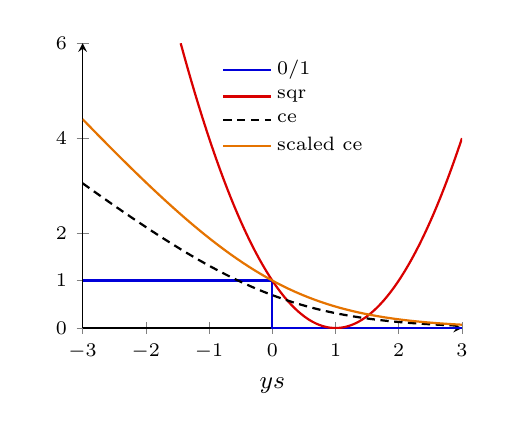
\begin{tikzpicture}
            \begin{axis}[
                width=6.4cm, height=5.2cm,
                xmin=-3, xmax=3, ymin=0, ymax=6,
                axis lines=left, xtick={-3,-2,-1,0,1,2,3}, ytick={0,1,2,4,6},
                tick label style={font=\scriptsize},
                xlabel={\(ys\)}, ylabel={\(\err\)}, label style={font=\small},
                legend style={font=\scriptsize, draw=none, fill=none,
                    at={(0.56,0.98)}, anchor=north},
                legend cell align=left]
                \addplot[blue!85!black, thick, const plot]
                    coordinates {(-3,1) (0,1) (0,0) (3,0)};
                \addplot[red!85!black, thick, domain=-1.449:3, samples=80]
                    {(x - 1)^2};
                \addplot[black, thick, densely dashed, domain=-3:3,
                    samples=60] {ln(1 + exp(-x))};
                \addplot[orange!90!black, thick, domain=-3:3, samples=60]
                    {ln(1 + exp(-x))/ln(2)};
                \legend{0/1, sqr, ce, scaled ce}
            \end{axis}
        \end{tikzpicture}
    \end{minipage}%
    \hfill
    \begin{minipage}[c]{0.53\textwidth}
        \raggedright
        \begin{itemize}
            \item 0/1: \(1\) iff \(ys \le 0\).
            \item \textcolor{red!85!black}{sqr}: large if \(ys \ll 1\),
                \textbf{but} over-charge \(ys \gg 1\);\\
                small \(\err_{\mathrm{SQR}} \to\) small \(\err_{0/1}\).
            \item ce: monotonic of \(ys\);\\
                small \(\err_{\mathrm{CE}} \leftrightarrow\) small
                \(\err_{0/1}\).
            \item \textcolor{orange!85!black}{scaled ce}: a proper upper bound
                of 0/1;\\
                small \(\err_{\mathrm{SCE}} \leftrightarrow\) small
                \(\err_{0/1}\).
        \end{itemize}
    \end{minipage}
\end{center}

\begin{itemize}
    \item \textbf{0/1 at \(ys = 0\)}: the convention \(\sign(0) \neq 1\) puts \(ys
        = 0\) on the wrong side, which is the safe reading: a score exactly on
        the boundary has not made a decision.
    \item \textbf{One-way arrow for sqr}: the parabola climbs again to the right
        of \(ys = 1\): an example classified correctly with a large margin still
        costs much squared error, so a small \(\err_{0/1}\) does not force a
        small \(\err_{\mathrm{SQR}}\).
    \item \textbf{Two-way arrows for ce}: both cross-entropy curves instead
        decrease monotonically in \(ys\), so pushing \(ys\) up lowers both
        errors at once.
    \item \textbf{Why scale}: plain ce is \emph{not} an upper bound: at \(ys = 0\)
        it equals \(\ln 2 < 1\). Dividing by \(\ln 2\) repairs exactly that.
\end{itemize}

\begin{proposition}[Scaled cross-entropy bounds 0/1 error]
    \label{prop:sce-bound}
    For \(y \in \{-1, +1\}\) and every real \(s\),
    \[
        \err_{0/1}(s, y) \le \err_{\mathrm{SCE}}(s, y) = \frac{1}{\ln 2}
        \err_{\mathrm{CE}}(s, y) .
    \]
\end{proposition}

\begin{proof}
    The equality is \(\log_2 u = \ln u / \ln 2\). Let \(\psi(t) = \log_2(1 +
    e^{-t})\); it is positive and strictly decreasing, since \(1 + e^{-t} > 1\)
    and \(e^{-t}\) decreases, and \(\psi(0) = \log_2 2 = 1\). If \(ys \le 0\),
    then \(\err_{0/1} = 1 = \psi(0) \le \psi(ys) = \err_{\mathrm{SCE}}\). If
    \(ys > 0\), then \(\err_{0/1} = 0 < \psi(ys)\).
\end{proof}

Together with \autoref{prop:sqr-bound}, both efficient models now minimise an
upper bound of the 0/1 error --- which is precisely what an algorithmic error
measure \(\errhat\) (\autoref{def:errhat}) is meant to do.

\begin{moral}
    \textcolor{orange!85!black}{Upper bound}: useful for designing algorithmic
    error \(\errhat\).
\end{moral}

\subsection{Theoretical Implication of Upper Bound}

For any \(ys\) where \(s = \bm{w}^\top \bm{x}\),
\begin{align*}
    &\err_{0/1}(s, y) \le \err_{\mathrm{SCE}}(s, y) = \frac{1}{\ln 2}
    \err_{\mathrm{CE}}(s, y)\\
    \Longrightarrow \quad
    &\Ein^{0/1}(\bm{w}) \le \Ein^{\mathrm{SCE}}(\bm{w}) = \frac{1}{\ln 2}
    \Ein^{\mathrm{CE}}(\bm{w})\\
    &\Eout^{0/1}(\bm{w}) \le \Eout^{\mathrm{SCE}}(\bm{w}) = \frac{1}{\ln 2}
    \Eout^{\mathrm{CE}}(\bm{w}) .
\end{align*}
The superscript names the pointwise error being averaged. \(\Ein\) is the mean
of the pointwise error over the \(N\) examples and \(\Eout\) its expectation
over \((\bm{x}, y) \sim P\); both are linear and preserve \(\le\), so the
pointwise inequality of \autoref{prop:sce-bound} passes to them term by term.

Two routes then lead to \(\Eout^{0/1}\):

\begin{center}
    \begin{adjustbox}{max width=\textwidth}
        \solidrules
        \begin{tabular}{@{}l|l@{}}
            \toprule
            \textbf{VC on \textcolor{blue}{0/1}:}
            & \textbf{VC-Reg on CE:}\\
            \midrule
            \(\begin{aligned}[t]
                \rule{0pt}{3ex}\Eout^{0/1}(\bm{w})
                &\le \Ein^{0/1}(\bm{w}) + \Omega^{0/1}\\
                &\le \tfrac{1}{\ln 2} \Ein^{\mathrm{CE}}(\bm{w}) +
                \Omega^{0/1}
            \end{aligned}\)
            & \(\begin{aligned}[t]
                \rule{0pt}{3ex}\Eout^{0/1}(\bm{w})
                &\le \tfrac{1}{\ln 2} \Eout^{\mathrm{CE}}(\bm{w})\\
                &\le \tfrac{1}{\ln 2} \Ein^{\mathrm{CE}}(\bm{w}) +
                \tfrac{1}{\ln 2} \Omega^{\mathrm{CE}}
            \end{aligned}\)\\[4pt]
            \bottomrule
        \end{tabular}
    \end{adjustbox}
\end{center}

\begin{itemize}
    \item \textbf{Left (VC on 0/1)}: \(\Omega^{0/1}\) is the penalty of
        \autoref{def:omega} for the perceptron set, \(\dvc = d + 1\). The VC
        bound of \autoref{thm:vc} holds with high probability for \emph{every}
        \(\bm{w}\) at once, so it covers the \(\bm{w}\) that logistic regression
        returns, even though logistic regression never looked at the 0/1 error;
        the second line is then \autoref{prop:sce-bound} averaged.
    \item \textbf{Right (VC-Reg on CE)}: the order is reversed: first bound
        \(\Eout^{0/1}\) by \(\Eout^{\mathrm{CE}}\), then generalise the
        cross-entropy error itself, with a penalty \(\Omega^{\mathrm{CE}}\) of
        the same kind for that real-valued error, which these notes do not
        derive.
\end{itemize}
Either way the right-hand side is small when \(\Ein^{\mathrm{CE}}(\bm{w})\) is,
and the same argument with \autoref{prop:sqr-bound} covers linear regression.

\begin{moral}
    Small \(\Ein^{\mathrm{CE}}(\bm{w}) \Longrightarrow\) small
    \(\Eout^{0/1}(\bm{w})\): \textbf{logistic/linear reg.} for
    \textcolor{blue}{linear classification}.
\end{moral}

\subsection{Regression for Classification}

\begin{enumerate}
    \item Run \textbf{logistic/linear reg.} on \(\mathcal{D}\) with \(y_n \in
        \left\{ -1, +1 \right\}\) to get \(\bm{w}_{\mathrm{REG}}\);
    \item return \(g(\bm{x}) = \sign(\bm{w}_{\mathrm{REG}}^\top \bm{x})\).
\end{enumerate}

This is the recipe of \autoref{sec:linreg-cls}, now with logistic regression as
a second choice. Against PLA, the three trade off as follows:

\begin{center}
    \begin{adjustbox}{max width=\textwidth}
        \solidrules
        \begin{tabular}{@{}>{\raggedright\arraybackslash}p{4.4cm}|>{\raggedright\arraybackslash}p{4.4cm}|>{\raggedright\arraybackslash}p{4.4cm}@{}}
            \toprule
            \textbf{PLA} & \textbf{linear regression}
            & \textbf{logistic regression}\\
            \midrule
            \textbullet\ pros:
            \textcolor{orange!85!black}{\textbf{efficient + strong guarantee
            if lin.\ separable}}
            & \textbullet\ pros: \textcolor{orange!85!black}{\textbf{`easiest'
            optimization}}
            & \textbullet\ pros: \textcolor{orange!85!black}{\textbf{`easy'
            optimization}}\\[3pt]
            \textbullet\ cons: works only if lin.\ separable, otherwise
            needing \textcolor{blue}{\textbf{pocket}} heuristic
            & \textbullet\ cons: loose bound of \(\err_{0/1}\) for large
            \(\abs{ys}\)
            & \textbullet\ cons: loose bound of \(\err_{0/1}\) for very
            negative \(ys\)\\
            \bottomrule
        \end{tabular}
    \end{adjustbox}
\end{center}

\begin{itemize}
    \item \textbf{`Easiest'}: linear regression is one pseudo-inverse
        (\autoref{alg:linreg}).
    \item \textbf{`Easy'}: logistic regression is a convex descent
        (\autoref{alg:logreg}).
\end{itemize}

Why is a loose bound a \emph{con}? Suppose a data point sits where the
regression error is much larger than \(\err_{0/1}\). For the regression error
this one point is very expensive, but for \(\err_{0/1}\) it is just one mistake
(or none), like any other point. So when we minimise the regression error,
\(\bm{w}\) may move a lot just to make this one point cheaper, and in doing so
push a few other points to the wrong side --- giving \emph{more} 0/1 mistakes.
This only matters if some data points really lie where the two errors are far
apart: \(\abs{ys}\) large on either side for squared error, and \(ys \ll 0\)
for cross-entropy, which goes to \(0\) on the correct side.

\begin{moral}
    \begin{itemize}
        \item \textcolor{red}{\textbf{linear regression}} sometimes used to
            \textcolor{red}{set \(\bm{w}_0\)} for
            \textcolor{blue}{\textbf{PLA/pocket/logistic regression}};
        \item \textcolor{blue}{\textbf{logistic regression}} often preferred
            over \textcolor{blue}{\textbf{pocket}}.
    \end{itemize}
\end{moral}

\begin{itemize}
    \item \textbf{Setting \(\bm{w}_0\)}: the use already suggested in
        \autoref{sec:linreg-cls}: a cheap, roughly right start.
    \item \textbf{Logistic regression over pocket}: both answer the
        non-separable case, but pocket is a heuristic search on an NP-hard
        problem, while logistic regression solves its own convex problem and,
        by the bound above, still controls the 0/1 error.
\end{itemize}

\begin{exercise}[Fun Time]
    Following the definition in the lecture, which of the following is not
    always \(\ge \err_{0/1}(y, s)\) when \(y \in \left\{ -1, +1 \right\}\)?
    \begin{enumerate}[(1)]
        \item \(\err_{0/1}(y, s)\);
        \item \(\err_{\mathrm{SQR}}(y, s)\);
        \item \(\err_{\mathrm{CE}}(y, s)\);
        \item \(\err_{\mathrm{SCE}}(y, s)\).
    \end{enumerate}
\end{exercise}

\begin{proof}[Reference Answer]
    (3). Too simple, uh? :-) Anyway, note that \(\err_{0/1}\) is surely an
    upper bound of itself. Choice (2) is \autoref{prop:sqr-bound} and choice (4)
    is \autoref{prop:sce-bound}. Choice (3) fails near the boundary: at \(ys =
    0\), \(\err_{\mathrm{CE}} = \ln 2 < 1 = \err_{0/1}\), and indeed
    \(\err_{\mathrm{CE}} < 1\) for all \(ys > -\ln(e - 1) \approx -0.54\).
\end{proof}

\section{Stochastic Gradient Descent}\label{sec:sgd}

\source{slides p.8--12}

Logistic regression is now justified as a classifier; what remains is its
cost, which is where PLA still wins.

\subsection{Two Iterative Optimization Schemes}

For \(t = 0, 1, \dots\)
\[
    \bm{w}_{t+1} \gets \bm{w}_t + \eta \bm{v} ;
\]
when stop, return last \(\bm{w}\) as \(g\).

\begin{center}
    \begin{adjustbox}{max width=\textwidth}
        \solidrules
        \begin{tabular}{@{}>{\raggedright\arraybackslash}p{6cm}|>{\raggedright\arraybackslash}p{6cm}@{}}
            \toprule
            \textbf{PLA} & \textbf{logistic regression
            \textcolor{blue}{(pocket)}}\\
            \midrule
            pick \((\bm{x}_n, y_n)\) and decide \(\bm{w}_{t+1}\) by
            \textcolor{orange!85!black}{\textbf{the one example}}
            & check \(\mathcal{D}\) and decide \(\bm{w}_{t+1}\)
            \textcolor{blue}{(or new \(\hat{\bm{w}}\))} by
            \textcolor{orange!85!black}{\textbf{all examples}}\\[2pt]
            \qquad \(O(1)\) time per iteration
            \textcolor{orange!85!black}{\textbf{:-)}}
            & \qquad \(O(N)\) time per iteration
            \textcolor{orange!85!black}{\textbf{:-(}}\\
            \bottomrule
        \end{tabular}
    \end{adjustbox}
\end{center}

\begin{itemize}
    \item \textbf{Logistic regression} needs all \(N\) examples because
        \(\nabla \Ein\) in \eqref{eq:lr-grad} is a sum over all of them.
    \item \textbf{Pocket} needs them because it compares \(\Ein\) of the new
        candidate with that of the one in its pocket (\autoref{alg:pocket}).
    \item \textbf{PLA}'s update, by contrast, touches a single example --- as in
        this update of a PLA run on data of my own:
\end{itemize}

\begin{center}
    \begin{minipage}[c]{0.5\textwidth}
        \centering
        \begin{tikzpicture}[scale=0.95]
            \fill[poshalf] (2.400,-1.049) -- (2.400,2.400) -- (-2.400,2.400) -- (-2.400,1.049) -- cycle;
            \fill[neghalf] (-2.400,-2.400) -- (2.400,-2.400) -- (2.400,-1.049) -- (-2.400,1.049) -- cycle;
            \draw[sepline] (2.400,-1.049) -- (-2.400,1.049);
            \draw[sepline, densely dashed, draw=Purple] (0.927,-2.400) -- (-0.927,2.400);
            \draw[plotbox] (-2.4,-2.4) rectangle (2.4,2.4);
            \foreach \p in {(-0.060,-1.051), (-1.533,-1.791), (-1.184,1.398), (0.570,-1.285), (-1.546,0.352), (-0.655,-0.913), (-1.569,-0.848), (-1.679,0.190), (0.152,-0.605)}{\node[dneg] at \p {\(\times\)};}
            \foreach \p in {(0.926,0.565), (1.817,-1.934), (1.407,-0.014), (0.989,0.715), (0.167,0.800), (1.169,-0.951), (1.752,1.325), (-0.147,1.968), (0.023,1.627)}{\node[dpos] at \p {};}
            \fill[black] (0,0) circle (1.2pt);
            \node[draw=SeaGreen!60!black, thick, circle, inner sep=0pt, minimum size=9pt] at (1.169,-0.951) {};
            \draw[-{Stealth[length=2mm]}, thick, black] (0,0) -- (1.169,-0.951);
            \draw[-{Stealth[length=2mm]}, very thick, red!75!black] (0,0) -- (0.737,1.687);
            \draw[-{Stealth[length=2mm]}, thick, densely dashed, SeaGreen!70!black] (0.737,1.687) -- (1.907,0.736);
            \draw[wvec] (0,0) -- (1.907,0.736);
            \node[font=\scriptsize, below left, inner sep=1pt] at (0,0) {\(O\)};
            \node[font=\scriptsize, text=red!75!black, inner sep=1pt, above]
                at (0.62,1.74) {\(\bm{w}_t\)};
            \node[font=\scriptsize, text=SeaGreen!50!black, inner sep=1pt, right]
                at (1.42,1.72) {\(y_n \bm{x}_n\)};
            \node[font=\scriptsize, text=Purple, inner sep=1pt, below]
                at (2.02,0.55) {\(\bm{w}_{t+1}\)};
            \node[font=\scriptsize, right] at (1.25,-0.80) {\(\bm{x}_n\)};
            \node[font=\scriptsize, right, align=left] at (2.45,-1.05)
                {line of\\\(\bm{w}_t\)};
            \node[font=\scriptsize, text=Purple, below] at (0.93,-2.45)
                {line of \(\bm{w}_{t+1}\)};
        \end{tikzpicture}
    \end{minipage}%
    \hfill
    \begin{minipage}[c]{0.46\textwidth}
        \begin{itemize}
            \item \textbf{Shading}: \(\bm{w}_t\)'s: blue where it predicts
                \(\dmark{o}\) (\(\bm{w}_t^\top \bm{x} > 0\)), red where it
                predicts \(\dmark{x}\).
            \item \textbf{Update}: \(\bm{w}_t\) gets three points wrong. PLA
                takes one of them, the circled \(\dmark{o}\) \(\bm{x}_n\) (\(y_n
                = +1\)) in the red half, and adds \(y_n \bm{x}_n\) (green,
                dashed) to \(\bm{w}_t\) (red), giving \(\bm{w}_{t+1}\) (purple),
                whose line is dashed. Afterwards only one point is wrong.
            \item \textbf{Origin}: as in \autoref{sec:pla}, the line passes
                through the origin \(O\), so the vectors can be drawn from
                \(O\).
        \end{itemize}
        The update is one vector addition, whatever \(N\) is.
    \end{minipage}
\end{center}

\begin{question}
    Logistic regression with \(O(1)\) time per iteration?
\end{question}

\subsection{Logistic Regression Revisited}

\[
    \bm{w}_{t+1} \gets \bm{w}_t + \eta \underbrace{\frac{1}{N} \sum_{n=1}^N
    \theta \left( -y_n \bm{w}_t^\top \bm{x}_n \right) \left( y_n \bm{x}_n
    \right)}_{-\nabla \Ein(\bm{w}_t)}
\]
\begin{itemize}
    \item Want: update direction \(\bm{v} \approx -\nabla \Ein(\bm{w}_t)\)
        while computing \(\bm{v}\) by \textcolor{orange!85!black}{one single
        \((\bm{x}_n, y_n)\)}.
    \item Technique on removing \(\frac{1}{N} \sum_{n=1}^N\): view as
        expectation \(\mathcal{E}\) over \textcolor{red}{uniform choice of
        \(n\)}!
\end{itemize}

Write \(\err(\bm{w}, \bm{x}_n, y_n)\) for the pointwise cross-entropy
\eqref{eq:ce-err}, so that
\[
    \Ein(\bm{w}) = \frac{1}{N} \sum_{n=1}^N \err(\bm{w}, \bm{x}_n, y_n) .
\] If \(n\) is drawn uniformly from \(\{1, \dots , N\}\), each
term has weight \(\frac{1}{N}\), so the average over \(n\) \emph{is} an
expectation, and the gradient passes through the finite sum:

\begin{definition}[Stochastic gradient]\label{def:stoch-grad}
    With \(n\) drawn uniformly at random from \(\{1, \dots , N\}\),
    \(\nabla_{\bm{w}} \err(\bm{w}, \bm{x}_n, y_n)\) is the \vocab{stochastic
    gradient}, and
    \[
        \nabla_{\bm{w}} \Ein(\bm{w}) = \mathop{\mathcal{E}}_{\text{random } n}
        \nabla_{\bm{w}} \err(\bm{w}, \bm{x}_n, y_n)
    \]
    is the \vocab{true gradient}.
\end{definition}

So instead of averaging the gradients of all \(N\) examples, each step picks
one \(n\) at random and takes the gradient of the error on that single example
only. It costs one example to compute, and it is right on average.

\subsection{Stochastic Gradient Descent (SGD)}

\begin{moral}
    \textcolor{orange!85!black}{Stochastic gradient} \(=\)
    \textcolor{blue}{true gradient} \(+\) \textcolor{red}{zero-mean `noise'
    directions}.
\end{moral}

That is, \(\nabla \err(\bm{w}, \bm{x}_n, y_n) = \nabla \Ein(\bm{w}) +
\bm{\epsilon}\) with \(\bm{\epsilon} = \nabla \err(\bm{w}, \bm{x}_n, y_n) -
\nabla \Ein(\bm{w})\), and \(\mathcal{E}_n \bm{\epsilon} = \bm{0}\) by
\autoref{def:stoch-grad}.

\begin{definition}[Stochastic gradient descent]\label{def:sgd}
    \vocab{Stochastic gradient descent} (SGD):
    \begin{itemize}
        \item idea: replace \textcolor{blue}{true gradient} by
            \textcolor{orange!85!black}{stochastic gradient};
        \item after enough steps, \textcolor{blue}{average true gradient}
            \(\approx\) \textcolor{orange!85!black}{average stochastic
            gradient};
        \item pros: \textcolor{orange!85!black}{\textbf{simple \& cheaper
            computation :-)}} --- useful for
            \textcolor{orange!85!black}{\textbf{big data}} or
            \textcolor{orange!85!black}{\textbf{online learning}};
        \item cons: less stable in nature.
    \end{itemize}
\end{definition}

The second bullet is what makes the replacement legitimate. Each step's noise
is zero-mean given everything before it, so the noise terms do not accumulate:
their average shrinks like \(1/\sqrt{T}\).

\begin{lemma}[Noise averages out]\label{lem:sgd-noise}
    Run SGD for \(T\) steps, drawing \(n_t\) uniformly and independently of
    the past at each step, and let \(\bm{\epsilon}_t = \nabla \err(\bm{w}_t,
    \bm{x}_{n_t}, y_{n_t}) - \nabla \Ein(\bm{w}_t)\). If \(\norm{\bm{\epsilon}_t}
    \le G\) always, then
    \[
        \mathcal{E} \norm{\frac{1}{T} \sum_{t=0}^{T-1} \bm{\epsilon}_t}^2 \le
        \frac{G^2}{T} .
    \]
\end{lemma}

\begin{proof}
    \(\bm{w}_t\) is determined by \(n_0, \dots , n_{t-1}\), and \(n_t\) is
    uniform and independent of these, so conditioned on them \(\mathcal{E}
    \bm{\epsilon}_t = \bm{0}\) by \autoref{def:stoch-grad}. For \(s < t\),
    \(\bm{\epsilon}_s\) is fixed once \(n_0, \dots , n_{t-1}\) are, hence
    \(\mathcal{E} \bigl[ \bm{\epsilon}_s^\top \bm{\epsilon}_t \bigr] =
    \mathcal{E} \bigl[ \bm{\epsilon}_s^\top \, \mathcal{E} [\bm{\epsilon}_t
    \mid n_0, \dots , n_{t-1}] \bigr] = 0\) by the tower property. Expanding
    the square, the cross terms vanish:
    \[
        \mathcal{E} \norm{\sum_{t=0}^{T-1} \bm{\epsilon}_t}^2 = \sum_{t=0}^{T-1}
        \mathcal{E} \norm{\bm{\epsilon}_t}^2 \le T G^2 ;
    \]
    divide by \(T^2\).
\end{proof}

\begin{itemize}
    \item \textbf{\(G\) exists for logistic regression}: \(\norm{\nabla
        \err(\bm{w}, \bm{x}_n, y_n)} = \theta(\cdot) \norm{\bm{x}_n} \le \max_n
        \norm{\bm{x}_n}\), the average \(\nabla \Ein\) obeys the same bound, and
        so \(G = 2 \max_n \norm{\bm{x}_n}\) works by the triangle inequality.
    \item \textbf{Average, not each step}: the lemma is about the \emph{average}
        over many steps; each single step can still point well away from
        \(-\nabla \Ein(\bm{w}_t)\), which is the instability of the last bullet.
\end{itemize}

SGD logistic regression, \textcolor{orange!85!black}{\textbf{looks familiar?
:-)}}:
\[
    \bm{w}_{t+1} \gets \bm{w}_t + \eta \underbrace{\theta \left( -y_n
    \bm{w}_t^\top \bm{x}_n \right) \left( y_n \bm{x}_n
    \right)}_{-\nabla \err(\bm{w}_t, \bm{x}_n, y_n)}
\]

The underbrace is one term of the sum in \eqref{eq:lr-grad}, negated and
without the \(\frac{1}{N}\). In full:

\begin{algorithm}[H]
    \caption{SGD Logistic Regression}\label{alg:sgd-logreg}
    \KwIn{training examples \(\mathcal{D}\), learning rate \(\eta\)}
    \KwOut{the last \(\bm{w}_{t+1}\), returned as \(g\)}
    initialize \(\bm{w}_0\)\;
    \For{\(t = 0, 1, \dots\)}{
        pick \(n \in \{1, \dots , N\}\) uniformly at random\;
        update by \(\bm{w}_{t+1} \gets \bm{w}_t + \eta \, \theta \left( -y_n
        \bm{w}_t^\top \bm{x}_n \right) \left( y_n \bm{x}_n \right)\)\;
        \lIf{\(t\) large enough}{\Return last \(\bm{w}_{t+1}\) as \(g\)}
    }
\end{algorithm}

Each iteration now costs \(O(d)\), independent of \(N\).

\subsection{PLA Revisited}

\begin{align*}
    \text{SGD logistic regression:} \quad
    \bm{w}_{t+1} &\gets \bm{w}_t + \textcolor{blue}{\eta} \cdot \theta \left(
    -y_n \bm{w}_t^\top \bm{x}_n \right)
    \textcolor{orange!85!black}{\left( y_n \bm{x}_n \right)}\\
    \text{PLA:} \quad
    \bm{w}_{t+1} &\gets \bm{w}_t + \textcolor{blue}{1} \cdot \llbracket y_n
    \neq \sign(\bm{w}_t^\top \bm{x}_n) \rrbracket
    \textcolor{orange!85!black}{\left( y_n \bm{x}_n \right)}
\end{align*}

\begin{moral}
    \begin{itemize}
        \item SGD logistic regression \(\approx\) `soft' PLA;
        \item PLA \(\approx\) SGD logistic regression with \(\eta = 1\) when
            \(\bm{w}_t^\top \bm{x}_n\) large.
    \end{itemize}
\end{moral}

Both move along \(y_n \bm{x}_n\) and differ only in the factor in front.
\begin{itemize}
    \item \textbf{PLA's factor}: \(1\) on a mistake and \(0\) otherwise.
    \item \textbf{SGD's factor}: \(\theta(-y_n \bm{w}_t^\top \bm{x}_n)\), which is
        near \(1\) when \(y_n \bm{w}_t^\top \bm{x}_n \ll 0\) (badly wrong) and
        near \(0\) when \(y_n \bm{w}_t^\top \bm{x}_n \gg 0\) (safely right) ---
        the Iverson bracket smoothed by \(\theta\).
\end{itemize}
The approximation is exact in the limit \(\abs{\bm{w}_t^\top \bm{x}_n} \to
\infty\), which is why it needs a large score.

Two practical rules of thumb:
\begin{itemize}
    \item stopping condition? \(t\) \textcolor{orange!85!black}{\textbf{large
        enough}};
    \item \(\eta\)? \textcolor{orange!85!black}{\(0.1\)} when \(\bm{x}\) in
        proper range.
\end{itemize}

\begin{itemize}
    \item \textbf{Stopping}: forced: checking \(\nabla \Ein(\bm{w}_t) \approx
        \bm{0}\), the stopping rule of \autoref{alg:logreg}, costs \(O(N)\) and
        would undo the saving.
    \item \textbf{\(\eta\)}: purely empirical: \(\eta = 0.1\) is not derived from
        anything, it is simply a value that tends to work in practice. It
        presumes the features are scaled to a moderate range, say \(\abs{x_i}
        \lesssim 1\), so that one step \(\eta \, \theta(\cdot) \, y_n
        \bm{x}_n\) changes each coordinate of \(\bm{w}\) by at most about
        \(0.1\).
\end{itemize}

\begin{exercise}[Fun Time]
    Consider applying SGD on linear regression for big data. What is the update
    direction when using the negative stochastic gradient?
    \begin{enumerate}[(1)]
        \item \(\bm{x}_n\);
        \item \(y_n \bm{x}_n\);
        \item \(2(\bm{w}_t^\top \bm{x}_n - y_n) \bm{x}_n\);
        \item \(2(y_n - \bm{w}_t^\top \bm{x}_n) \bm{x}_n\).
    \end{enumerate}
\end{exercise}

\begin{proof}[Reference Answer]
    (4). Go check \autoref{sec:linreg-algo} if you have forgotten about the
    gradient of squared error. :-) For one example, \(\err(\bm{w}, \bm{x}_n,
    y_n) = (\bm{w}^\top \bm{x}_n - y_n)^2\) has gradient \(2(\bm{w}^\top
    \bm{x}_n - y_n) \bm{x}_n\) by the chain rule; its negative is (4).
    Anyway, the update rule has a nice physical interpretation: improve
    \(\bm{w}_t\) by `correcting' proportional to the residual \((y_n -
    \bm{w}_t^\top \bm{x}_n)\).
\end{proof}

\section{Multiclass via Logistic Regression}\label{sec:multi-logreg}

\source{slides p.13--19}

Every tool so far answers a yes/no question. The multiclass problems of
\autoref{def:multiclass} ask for one of \(K\) labels.

\subsection{Multiclass Classification}

\begin{center}
    \begin{minipage}[c]{0.36\textwidth}
        \centering
\begin{tikzpicture}[scale=0.8]
    \foreach \p in {(2.301,3.090), (2.680,3.020), (2.829,2.902), (2.969,2.980), (2.392,2.800), (2.590,2.776), (3.101,2.651), (3.563,2.471), (3.728,2.533), (3.291,2.337)}{\node[mcsq] at \p {};}
    \foreach \p in {(1.361,3.608), (1.171,2.996), (0.701,3.020), (0.371,2.941), (0.511,2.808), (1.493,2.714), (0.907,2.706), (1.724,2.478)}{\node[mcdia] at \p {};}
    \foreach \p in {(0.544,1.467), (1.014,1.451), (1.435,1.451), (0.775,1.271), (0.313,0.769), (0.759,0.675), (1.023,0.675), (1.419,0.706), (1.551,0.549), (1.592,0.275)}{\node[mctri] at \p {};}
    \foreach \p in {(2.392,2.055), (3.093,1.467), (2.647,1.443), (3.456,1.302), (3.109,1.200), (3.109,0.965), (3.365,0.722), (3.365,0.455), (3.777,0.533), (2.507,0.463)}{\node[mcstar] at \p {};}
    \draw[plotbox] (0,0) rectangle (4.0,4.0);
\end{tikzpicture}
    \end{minipage}%
    \hfill
    \begin{minipage}[c]{0.6\textwidth}
        \raggedright
        \begin{itemize}
            \item \(\mathcal{Y} = \left\{ \mcmark{sq}, \mcmark{dia},
                \mcmark{tri}, \mcmark{star} \right\}\) (4-class
                classification);
            \item \textcolor{orange!85!black}{\textbf{many applications}} in
                practice, especially for `recognition'.
        \end{itemize}
    \end{minipage}
\end{center}

The coin data of \autoref{eg:coins} looked just like this.
\begin{itemize}
    \item \textbf{Data}: the data set drawn here, and in every figure of this
        section and the next, is mine: \(N = 38\) points (\(10\) each of
        \(\mcmark{sq}\), \(\mcmark{tri}\), \(\mcmark{star}\) and \(8\) of
        \(\mcmark{dia}\)) placed where the deck's markers sit.
    \item \textbf{Classifiers}: every boundary and shade drawn on it is
        computed, not sketched: each binary classifier is logistic regression
        by \autoref{alg:logreg} with \(\bm{w}_0 = \bm{0}\), \(\eta = 1\) and
        \(150\) steps, on the two coordinates rescaled to \([-1, 1]\).
\end{itemize}

\begin{moral}
    Next: use \textcolor{orange!85!black}{\textbf{tools for
    \(\{\)\dmark{x}, \dmark{o}\(\}\) classification}} to \(\{\)\mcmark{sq},
    \mcmark{dia}, \mcmark{tri}, \mcmark{star}\(\}\) classification.
\end{moral}

\subsection{One Class at a Time}

Ask one yes/no question per class: is it \(\mcmark{sq}\) or not? Relabel that
class \(\dmark{o}\) and all the others \(\dmark{x}\), and learn a binary
classifier. Four classes, four relabellings of the same \(38\) points:

\begin{center}
    \begin{adjustbox}{max width=\textwidth}
        \setlength{\tabcolsep}{4pt}\scriptsize
        \begin{tabular}{@{}cccc@{}}
            \begin{tikzpicture}[scale=0.8]
                \fill[poshalf] (4.000,1.215) -- (4.000,4.000) -- (0.853,4.000) -- cycle;
                \fill[neghalf] (0.000,0.000) -- (4.000,0.000) -- (4.000,1.215) -- (0.853,4.000) -- (0.000,4.000) -- cycle;
                \draw[sepline] (4.000,1.215) -- (0.853,4.000);
                \foreach \p in {(2.301,3.090), (2.680,3.020), (2.829,2.902), (2.969,2.980), (2.392,2.800), (2.590,2.776), (3.101,2.651), (3.563,2.471), (3.728,2.533), (3.291,2.337)}{\node[dpos] at \p {};}
                \foreach \p in {(1.361,3.608), (1.171,2.996), (0.701,3.020), (0.371,2.941), (0.511,2.808), (1.493,2.714), (0.907,2.706), (1.724,2.478)}{\node[dneg] at \p {\(\times\)};}
                \foreach \p in {(0.544,1.467), (1.014,1.451), (1.435,1.451), (0.775,1.271), (0.313,0.769), (0.759,0.675), (1.023,0.675), (1.419,0.706), (1.551,0.549), (1.592,0.275)}{\node[dneg] at \p {\(\times\)};}
                \foreach \p in {(2.392,2.055), (3.093,1.467), (2.647,1.443), (3.456,1.302), (3.109,1.200), (3.109,0.965), (3.365,0.722), (3.365,0.455), (3.777,0.533), (2.507,0.463)}{\node[dneg] at \p {\(\times\)};}
                \draw[plotbox] (0,0) rectangle (4.0,4.0);
            \end{tikzpicture} &
            \begin{tikzpicture}[scale=0.8]
                \fill[poshalf] (3.045,4.000) -- (0.000,4.000) -- (0.000,1.356) -- cycle;
                \fill[neghalf] (0.000,0.000) -- (4.000,0.000) -- (4.000,4.000) -- (3.045,4.000) -- (0.000,1.356) -- cycle;
                \draw[sepline] (3.045,4.000) -- (0.000,1.356);
                \foreach \p in {(2.301,3.090), (2.680,3.020), (2.829,2.902), (2.969,2.980), (2.392,2.800), (2.590,2.776), (3.101,2.651), (3.563,2.471), (3.728,2.533), (3.291,2.337)}{\node[dneg] at \p {\(\times\)};}
                \foreach \p in {(1.361,3.608), (1.171,2.996), (0.701,3.020), (0.371,2.941), (0.511,2.808), (1.493,2.714), (0.907,2.706), (1.724,2.478)}{\node[dpos] at \p {};}
                \foreach \p in {(0.544,1.467), (1.014,1.451), (1.435,1.451), (0.775,1.271), (0.313,0.769), (0.759,0.675), (1.023,0.675), (1.419,0.706), (1.551,0.549), (1.592,0.275)}{\node[dneg] at \p {\(\times\)};}
                \foreach \p in {(2.392,2.055), (3.093,1.467), (2.647,1.443), (3.456,1.302), (3.109,1.200), (3.109,0.965), (3.365,0.722), (3.365,0.455), (3.777,0.533), (2.507,0.463)}{\node[dneg] at \p {\(\times\)};}
                \draw[plotbox] (0,0) rectangle (4.0,4.0);
            \end{tikzpicture} &
            \begin{tikzpicture}[scale=0.8]
                \fill[poshalf] (0.000,0.000) -- (2.913,0.000) -- (0.000,2.816) -- cycle;
                \fill[neghalf] (2.913,0.000) -- (4.000,0.000) -- (4.000,4.000) -- (0.000,4.000) -- (0.000,2.816) -- cycle;
                \draw[sepline] (2.913,0.000) -- (0.000,2.816);
                \foreach \p in {(2.301,3.090), (2.680,3.020), (2.829,2.902), (2.969,2.980), (2.392,2.800), (2.590,2.776), (3.101,2.651), (3.563,2.471), (3.728,2.533), (3.291,2.337)}{\node[dneg] at \p {\(\times\)};}
                \foreach \p in {(1.361,3.608), (1.171,2.996), (0.701,3.020), (0.371,2.941), (0.511,2.808), (1.493,2.714), (0.907,2.706), (1.724,2.478)}{\node[dneg] at \p {\(\times\)};}
                \foreach \p in {(0.544,1.467), (1.014,1.451), (1.435,1.451), (0.775,1.271), (0.313,0.769), (0.759,0.675), (1.023,0.675), (1.419,0.706), (1.551,0.549), (1.592,0.275)}{\node[dpos] at \p {};}
                \foreach \p in {(2.392,2.055), (3.093,1.467), (2.647,1.443), (3.456,1.302), (3.109,1.200), (3.109,0.965), (3.365,0.722), (3.365,0.455), (3.777,0.533), (2.507,0.463)}{\node[dneg] at \p {\(\times\)};}
                \draw[plotbox] (0,0) rectangle (4.0,4.0);
            \end{tikzpicture} &
            \begin{tikzpicture}[scale=0.8]
                \fill[poshalf] (1.453,0.000) -- (4.000,0.000) -- (4.000,2.749) -- cycle;
                \fill[neghalf] (0.000,0.000) -- (1.453,0.000) -- (4.000,2.749) -- (4.000,4.000) -- (0.000,4.000) -- cycle;
                \draw[sepline] (1.453,0.000) -- (4.000,2.749);
                \foreach \p in {(2.301,3.090), (2.680,3.020), (2.829,2.902), (2.969,2.980), (2.392,2.800), (2.590,2.776), (3.101,2.651), (3.563,2.471), (3.728,2.533), (3.291,2.337)}{\node[dneg] at \p {\(\times\)};}
                \foreach \p in {(1.361,3.608), (1.171,2.996), (0.701,3.020), (0.371,2.941), (0.511,2.808), (1.493,2.714), (0.907,2.706), (1.724,2.478)}{\node[dneg] at \p {\(\times\)};}
                \foreach \p in {(0.544,1.467), (1.014,1.451), (1.435,1.451), (0.775,1.271), (0.313,0.769), (0.759,0.675), (1.023,0.675), (1.419,0.706), (1.551,0.549), (1.592,0.275)}{\node[dneg] at \p {\(\times\)};}
                \foreach \p in {(2.392,2.055), (3.093,1.467), (2.647,1.443), (3.456,1.302), (3.109,1.200), (3.109,0.965), (3.365,0.722), (3.365,0.455), (3.777,0.533), (2.507,0.463)}{\node[dpos] at \p {};}
                \draw[plotbox] (0,0) rectangle (4.0,4.0);
            \end{tikzpicture}\\
            \mcmark{sq} or not? &
            \mcmark{dia} or not? &
            \mcmark{tri} or not? &
            \mcmark{star} or not?\\
            \{\mcmark{sq} = \dmark{o}, \mcmark{dia} = \dmark{x}, \mcmark{tri} = \dmark{x}, \mcmark{star} = \dmark{x}\} &
            \{\mcmark{sq} = \dmark{x}, \mcmark{dia} = \dmark{o}, \mcmark{tri} = \dmark{x}, \mcmark{star} = \dmark{x}\} &
            \{\mcmark{sq} = \dmark{x}, \mcmark{dia} = \dmark{x}, \mcmark{tri} = \dmark{o}, \mcmark{star} = \dmark{x}\} &
            \{\mcmark{sq} = \dmark{x}, \mcmark{dia} = \dmark{x}, \mcmark{tri} = \dmark{x}, \mcmark{star} = \dmark{o}\}
        \end{tabular}
    \end{adjustbox}
\end{center}

Each classifier separates its own class from the rest fairly well, getting one
or two points wrong near the middle of the square, where the classes come
close. The question is what to do with four answers.

\subsection{Multiclass Prediction: Combine Binary Classifiers}

Predict \(k\) where exactly one classifier says \(\dmark{o}\) and it is the
\(k\)-th one. The four half-planes above, overlaid:

\begin{center}
    \begin{adjustbox}{max width=\textwidth}
        \begin{tikzpicture}[scale=0.75]
            \begin{scope}[shift={(0.000,2.125)}, scale=0.45, transform shape]
                \fill[poshalf] (4.000,1.215) -- (4.000,4.000) -- (0.853,4.000) -- cycle;
                \fill[neghalf] (0.000,0.000) -- (4.000,0.000) -- (4.000,1.215) -- (0.853,4.000) -- (0.000,4.000) -- cycle;
                \draw[sepline] (4.000,1.215) -- (0.853,4.000);
                \foreach \p in {(2.301,3.090), (2.680,3.020), (2.829,2.902), (2.969,2.980), (2.392,2.800), (2.590,2.776), (3.101,2.651), (3.563,2.471), (3.728,2.533), (3.291,2.337)}{\node[dpos] at \p {};}
                \foreach \p in {(1.361,3.608), (1.171,2.996), (0.701,3.020), (0.371,2.941), (0.511,2.808), (1.493,2.714), (0.907,2.706), (1.724,2.478)}{\node[dneg] at \p {\(\times\)};}
                \foreach \p in {(0.544,1.467), (1.014,1.451), (1.435,1.451), (0.775,1.271), (0.313,0.769), (0.759,0.675), (1.023,0.675), (1.419,0.706), (1.551,0.549), (1.592,0.275)}{\node[dneg] at \p {\(\times\)};}
                \foreach \p in {(2.392,2.055), (3.093,1.467), (2.647,1.443), (3.456,1.302), (3.109,1.200), (3.109,0.965), (3.365,0.722), (3.365,0.455), (3.777,0.533), (2.507,0.463)}{\node[dneg] at \p {\(\times\)};}
                \draw[plotbox] (0,0) rectangle (4.0,4.0);
            \end{scope}
            \begin{scope}[shift={(2.050,2.125)}, scale=0.45, transform shape]
                \fill[poshalf] (3.045,4.000) -- (0.000,4.000) -- (0.000,1.356) -- cycle;
                \fill[neghalf] (0.000,0.000) -- (4.000,0.000) -- (4.000,4.000) -- (3.045,4.000) -- (0.000,1.356) -- cycle;
                \draw[sepline] (3.045,4.000) -- (0.000,1.356);
                \foreach \p in {(2.301,3.090), (2.680,3.020), (2.829,2.902), (2.969,2.980), (2.392,2.800), (2.590,2.776), (3.101,2.651), (3.563,2.471), (3.728,2.533), (3.291,2.337)}{\node[dneg] at \p {\(\times\)};}
                \foreach \p in {(1.361,3.608), (1.171,2.996), (0.701,3.020), (0.371,2.941), (0.511,2.808), (1.493,2.714), (0.907,2.706), (1.724,2.478)}{\node[dpos] at \p {};}
                \foreach \p in {(0.544,1.467), (1.014,1.451), (1.435,1.451), (0.775,1.271), (0.313,0.769), (0.759,0.675), (1.023,0.675), (1.419,0.706), (1.551,0.549), (1.592,0.275)}{\node[dneg] at \p {\(\times\)};}
                \foreach \p in {(2.392,2.055), (3.093,1.467), (2.647,1.443), (3.456,1.302), (3.109,1.200), (3.109,0.965), (3.365,0.722), (3.365,0.455), (3.777,0.533), (2.507,0.463)}{\node[dneg] at \p {\(\times\)};}
                \draw[plotbox] (0,0) rectangle (4.0,4.0);
            \end{scope}
            \begin{scope}[shift={(0.000,0.075)}, scale=0.45, transform shape]
                \fill[poshalf] (0.000,0.000) -- (2.913,0.000) -- (0.000,2.816) -- cycle;
                \fill[neghalf] (2.913,0.000) -- (4.000,0.000) -- (4.000,4.000) -- (0.000,4.000) -- (0.000,2.816) -- cycle;
                \draw[sepline] (2.913,0.000) -- (0.000,2.816);
                \foreach \p in {(2.301,3.090), (2.680,3.020), (2.829,2.902), (2.969,2.980), (2.392,2.800), (2.590,2.776), (3.101,2.651), (3.563,2.471), (3.728,2.533), (3.291,2.337)}{\node[dneg] at \p {\(\times\)};}
                \foreach \p in {(1.361,3.608), (1.171,2.996), (0.701,3.020), (0.371,2.941), (0.511,2.808), (1.493,2.714), (0.907,2.706), (1.724,2.478)}{\node[dneg] at \p {\(\times\)};}
                \foreach \p in {(0.544,1.467), (1.014,1.451), (1.435,1.451), (0.775,1.271), (0.313,0.769), (0.759,0.675), (1.023,0.675), (1.419,0.706), (1.551,0.549), (1.592,0.275)}{\node[dpos] at \p {};}
                \foreach \p in {(2.392,2.055), (3.093,1.467), (2.647,1.443), (3.456,1.302), (3.109,1.200), (3.109,0.965), (3.365,0.722), (3.365,0.455), (3.777,0.533), (2.507,0.463)}{\node[dneg] at \p {\(\times\)};}
                \draw[plotbox] (0,0) rectangle (4.0,4.0);
            \end{scope}
            \begin{scope}[shift={(2.050,0.075)}, scale=0.45, transform shape]
                \fill[poshalf] (1.453,0.000) -- (4.000,0.000) -- (4.000,2.749) -- cycle;
                \fill[neghalf] (0.000,0.000) -- (1.453,0.000) -- (4.000,2.749) -- (4.000,4.000) -- (0.000,4.000) -- cycle;
                \draw[sepline] (1.453,0.000) -- (4.000,2.749);
                \foreach \p in {(2.301,3.090), (2.680,3.020), (2.829,2.902), (2.969,2.980), (2.392,2.800), (2.590,2.776), (3.101,2.651), (3.563,2.471), (3.728,2.533), (3.291,2.337)}{\node[dneg] at \p {\(\times\)};}
                \foreach \p in {(1.361,3.608), (1.171,2.996), (0.701,3.020), (0.371,2.941), (0.511,2.808), (1.493,2.714), (0.907,2.706), (1.724,2.478)}{\node[dneg] at \p {\(\times\)};}
                \foreach \p in {(0.544,1.467), (1.014,1.451), (1.435,1.451), (0.775,1.271), (0.313,0.769), (0.759,0.675), (1.023,0.675), (1.419,0.706), (1.551,0.549), (1.592,0.275)}{\node[dneg] at \p {\(\times\)};}
                \foreach \p in {(2.392,2.055), (3.093,1.467), (2.647,1.443), (3.456,1.302), (3.109,1.200), (3.109,0.965), (3.365,0.722), (3.365,0.455), (3.777,0.533), (2.507,0.463)}{\node[dpos] at \p {};}
                \draw[plotbox] (0,0) rectangle (4.0,4.0);
            \end{scope}
            \draw[mlarrow] (4.100,2) -- (4.900,2);
            \begin{scope}[shift={(5.150,0)}]
                \fill[tieregion] (3.045,4.000) -- (0.853,4.000) -- (1.939,3.039) -- cycle;
                \fill[tieregion] (4.000,1.215) -- (4.000,2.749) -- (3.219,1.906) -- cycle;
                \fill[rgsq, draw=rgsq, line width=0.1pt] (4.000,2.749) -- (4.000,4.000) -- (3.045,4.000) -- (1.939,3.039) -- (3.219,1.906) -- cycle;
                \fill[tieregion] (0.000,2.816) -- (0.000,1.356) -- (0.796,2.047) -- cycle;
                \fill[rgdia, draw=rgdia, line width=0.1pt] (1.939,3.039) -- (0.853,4.000) -- (0.000,4.000) -- (0.000,2.816) -- (0.796,2.047) -- cycle;
                \fill[tieregion] (1.453,0.000) -- (2.913,0.000) -- (2.143,0.745) -- cycle;
                \fill[rgtri, draw=rgtri, line width=0.1pt] (0.000,0.000) -- (1.453,0.000) -- (2.143,0.745) -- (0.796,2.047) -- (0.000,1.356) -- cycle;
                \fill[rgstar, draw=rgstar, line width=0.1pt] (2.913,0.000) -- (4.000,0.000) -- (4.000,1.215) -- (3.219,1.906) -- (2.143,0.745) -- cycle;
                \fill[tieregion] (3.219,1.906) -- (1.939,3.039) -- (0.796,2.047) -- (2.143,0.745) -- cycle;
                \foreach \p in {(2.301,3.090), (2.680,3.020), (2.829,2.902), (2.969,2.980), (2.392,2.800), (2.590,2.776), (3.101,2.651), (3.563,2.471), (3.728,2.533), (3.291,2.337)}{\node[mcsq] at \p {};}
                \foreach \p in {(1.361,3.608), (1.171,2.996), (0.701,3.020), (0.371,2.941), (0.511,2.808), (1.493,2.714), (0.907,2.706), (1.724,2.478)}{\node[mcdia] at \p {};}
                \foreach \p in {(0.544,1.467), (1.014,1.451), (1.435,1.451), (0.775,1.271), (0.313,0.769), (0.759,0.675), (1.023,0.675), (1.419,0.706), (1.551,0.549), (1.592,0.275)}{\node[mctri] at \p {};}
                \foreach \p in {(2.392,2.055), (3.093,1.467), (2.647,1.443), (3.456,1.302), (3.109,1.200), (3.109,0.965), (3.365,0.722), (3.365,0.455), (3.777,0.533), (2.507,0.463)}{\node[mcstar] at \p {};}
                \draw[plotbox] (0,0) rectangle (4.0,4.0);
            \end{scope}
            \fill[tieregion] (9.400,1.75) rectangle ++(0.5,0.5);
            \draw[plotbox] (9.400,1.75) rectangle ++(0.5,0.5);
            \node[right, font=\scriptsize] at (9.950,2) {tie};
        \end{tikzpicture}
    \end{adjustbox}
\end{center}

\begin{question}
    But ties? :-)
\end{question}

The coloured regions are where exactly one classifier claims the input. The
hatched ones are not: in the middle all four say \(\dmark{x}\), and along the
diagonals two say \(\dmark{o}\) at once. Together these take up about a third
of the square, and there the hard answers give no reason to prefer any class.

\subsection{One Class at a Time Softly}

Instead of `\(\mcmark{sq}\) or not?', ask `how likely is \(\mcmark{sq}\)?'.
That is, use each logistic regression as a soft binary classifier
(\autoref{def:soft-binary}) on the same relabelled data: \(\theta(\bm{w}_{[k]}^\top
\bm{x})\) estimates \(P(k \mid \bm{x})\), the probability that \(\bm{x}\) belongs
to class \(k\), instead of only answering yes or no.

\begin{center}
    \begin{adjustbox}{max width=\textwidth}
        \setlength{\tabcolsep}{4pt}\scriptsize
        \begin{tabular}{@{}cccc@{}}
            \begin{tikzpicture}[scale=0.8]
                \fill[red!45!white, draw=red!45!white, line width=0.1pt] (0.000,0.000) -- (2.659,0.000) -- (0.000,2.353) -- cycle;
                \fill[red!45!white, draw=red!45!white, line width=0.1pt] (2.659,0.000) -- (2.749,0.000) -- (0.000,2.433) -- (0.000,2.353) -- cycle;
                \fill[red!45!white, draw=red!45!white, line width=0.1pt] (2.749,0.000) -- (2.839,0.000) -- (0.000,2.513) -- (0.000,2.433) -- cycle;
                \fill[red!45!white, draw=red!45!white, line width=0.1pt] (2.839,0.000) -- (2.930,0.000) -- (0.000,2.593) -- (0.000,2.513) -- cycle;
                \fill[red!45!white, draw=red!45!white, line width=0.1pt] (2.930,0.000) -- (3.020,0.000) -- (0.000,2.673) -- (0.000,2.593) -- cycle;
                \fill[red!44!white, draw=red!44!white, line width=0.1pt] (3.020,0.000) -- (3.111,0.000) -- (0.000,2.753) -- (0.000,2.673) -- cycle;
                \fill[red!44!white, draw=red!44!white, line width=0.1pt] (3.111,0.000) -- (3.201,0.000) -- (0.000,2.833) -- (0.000,2.753) -- cycle;
                \fill[red!44!white, draw=red!44!white, line width=0.1pt] (3.201,0.000) -- (3.292,0.000) -- (0.000,2.913) -- (0.000,2.833) -- cycle;
                \fill[red!44!white, draw=red!44!white, line width=0.1pt] (3.292,0.000) -- (3.382,0.000) -- (0.000,2.993) -- (0.000,2.913) -- cycle;
                \fill[red!44!white, draw=red!44!white, line width=0.1pt] (3.382,0.000) -- (3.473,0.000) -- (0.000,3.074) -- (0.000,2.993) -- cycle;
                \fill[red!44!white, draw=red!44!white, line width=0.1pt] (3.473,0.000) -- (3.563,0.000) -- (0.000,3.154) -- (0.000,3.074) -- cycle;
                \fill[red!43!white, draw=red!43!white, line width=0.1pt] (3.563,0.000) -- (3.654,0.000) -- (0.000,3.234) -- (0.000,3.154) -- cycle;
                \fill[red!43!white, draw=red!43!white, line width=0.1pt] (3.654,0.000) -- (3.744,0.000) -- (0.000,3.314) -- (0.000,3.234) -- cycle;
                \fill[red!42!white, draw=red!42!white, line width=0.1pt] (3.744,0.000) -- (3.835,0.000) -- (0.000,3.394) -- (0.000,3.314) -- cycle;
                \fill[red!42!white, draw=red!42!white, line width=0.1pt] (3.835,0.000) -- (3.925,0.000) -- (0.000,3.474) -- (0.000,3.394) -- cycle;
                \fill[red!41!white, draw=red!41!white, line width=0.1pt] (3.925,0.000) -- (4.000,0.000) -- (4.000,0.014) -- (0.000,3.554) -- (0.000,3.474) -- cycle;
                \fill[red!40!white, draw=red!40!white, line width=0.1pt] (4.000,0.014) -- (4.000,0.094) -- (0.000,3.634) -- (0.000,3.554) -- cycle;
                \fill[red!39!white, draw=red!39!white, line width=0.1pt] (4.000,0.094) -- (4.000,0.174) -- (0.000,3.714) -- (0.000,3.634) -- cycle;
                \fill[red!38!white, draw=red!38!white, line width=0.1pt] (4.000,0.174) -- (4.000,0.254) -- (0.000,3.794) -- (0.000,3.714) -- cycle;
                \fill[red!37!white, draw=red!37!white, line width=0.1pt] (4.000,0.254) -- (4.000,0.334) -- (0.000,3.874) -- (0.000,3.794) -- cycle;
                \fill[red!35!white, draw=red!35!white, line width=0.1pt] (4.000,0.334) -- (4.000,0.414) -- (0.000,3.954) -- (0.000,3.874) -- cycle;
                \fill[red!33!white, draw=red!33!white, line width=0.1pt] (4.000,0.414) -- (4.000,0.494) -- (0.039,4.000) -- (0.000,4.000) -- (0.000,3.954) -- cycle;
                \fill[red!31!white, draw=red!31!white, line width=0.1pt] (4.000,0.494) -- (4.000,0.574) -- (0.129,4.000) -- (0.039,4.000) -- cycle;
                \fill[red!29!white, draw=red!29!white, line width=0.1pt] (4.000,0.574) -- (4.000,0.654) -- (0.220,4.000) -- (0.129,4.000) -- cycle;
                \fill[red!26!white, draw=red!26!white, line width=0.1pt] (4.000,0.654) -- (4.000,0.735) -- (0.310,4.000) -- (0.220,4.000) -- cycle;
                \fill[red!23!white, draw=red!23!white, line width=0.1pt] (4.000,0.735) -- (4.000,0.815) -- (0.401,4.000) -- (0.310,4.000) -- cycle;
                \fill[red!19!white, draw=red!19!white, line width=0.1pt] (4.000,0.815) -- (4.000,0.895) -- (0.491,4.000) -- (0.401,4.000) -- cycle;
                \fill[red!15!white, draw=red!15!white, line width=0.1pt] (4.000,0.895) -- (4.000,0.975) -- (0.582,4.000) -- (0.491,4.000) -- cycle;
                \fill[red!11!white, draw=red!11!white, line width=0.1pt] (4.000,0.975) -- (4.000,1.055) -- (0.672,4.000) -- (0.582,4.000) -- cycle;
                \fill[red!7!white, draw=red!7!white, line width=0.1pt] (4.000,1.055) -- (4.000,1.135) -- (0.763,4.000) -- (0.672,4.000) -- cycle;
                \fill[red!2!white, draw=red!2!white, line width=0.1pt] (4.000,1.135) -- (4.000,1.215) -- (0.853,4.000) -- (0.763,4.000) -- cycle;
                \fill[blue!2!white, draw=blue!2!white, line width=0.1pt] (4.000,1.215) -- (4.000,1.295) -- (0.944,4.000) -- (0.853,4.000) -- cycle;
                \fill[blue!7!white, draw=blue!7!white, line width=0.1pt] (4.000,1.295) -- (4.000,1.375) -- (1.034,4.000) -- (0.944,4.000) -- cycle;
                \fill[blue!11!white, draw=blue!11!white, line width=0.1pt] (4.000,1.375) -- (4.000,1.455) -- (1.125,4.000) -- (1.034,4.000) -- cycle;
                \fill[blue!15!white, draw=blue!15!white, line width=0.1pt] (4.000,1.455) -- (4.000,1.535) -- (1.215,4.000) -- (1.125,4.000) -- cycle;
                \fill[blue!19!white, draw=blue!19!white, line width=0.1pt] (4.000,1.535) -- (4.000,1.615) -- (1.306,4.000) -- (1.215,4.000) -- cycle;
                \fill[blue!23!white, draw=blue!23!white, line width=0.1pt] (4.000,1.615) -- (4.000,1.695) -- (1.396,4.000) -- (1.306,4.000) -- cycle;
                \fill[blue!26!white, draw=blue!26!white, line width=0.1pt] (4.000,1.695) -- (4.000,1.776) -- (1.486,4.000) -- (1.396,4.000) -- cycle;
                \fill[blue!29!white, draw=blue!29!white, line width=0.1pt] (4.000,1.776) -- (4.000,1.856) -- (1.577,4.000) -- (1.486,4.000) -- cycle;
                \fill[blue!31!white, draw=blue!31!white, line width=0.1pt] (4.000,1.856) -- (4.000,1.936) -- (1.667,4.000) -- (1.577,4.000) -- cycle;
                \fill[blue!33!white, draw=blue!33!white, line width=0.1pt] (4.000,1.936) -- (4.000,2.016) -- (1.758,4.000) -- (1.667,4.000) -- cycle;
                \fill[blue!35!white, draw=blue!35!white, line width=0.1pt] (4.000,2.016) -- (4.000,2.096) -- (1.848,4.000) -- (1.758,4.000) -- cycle;
                \fill[blue!37!white, draw=blue!37!white, line width=0.1pt] (4.000,2.096) -- (4.000,2.176) -- (1.939,4.000) -- (1.848,4.000) -- cycle;
                \fill[blue!38!white, draw=blue!38!white, line width=0.1pt] (4.000,2.176) -- (4.000,2.256) -- (2.029,4.000) -- (1.939,4.000) -- cycle;
                \fill[blue!39!white, draw=blue!39!white, line width=0.1pt] (4.000,2.256) -- (4.000,2.336) -- (2.120,4.000) -- (2.029,4.000) -- cycle;
                \fill[blue!40!white, draw=blue!40!white, line width=0.1pt] (4.000,2.336) -- (4.000,2.416) -- (2.210,4.000) -- (2.120,4.000) -- cycle;
                \fill[blue!41!white, draw=blue!41!white, line width=0.1pt] (4.000,2.416) -- (4.000,2.496) -- (2.301,4.000) -- (2.210,4.000) -- cycle;
                \fill[blue!42!white, draw=blue!42!white, line width=0.1pt] (4.000,2.496) -- (4.000,2.576) -- (2.391,4.000) -- (2.301,4.000) -- cycle;
                \fill[blue!42!white, draw=blue!42!white, line width=0.1pt] (4.000,2.576) -- (4.000,2.656) -- (2.482,4.000) -- (2.391,4.000) -- cycle;
                \fill[blue!43!white, draw=blue!43!white, line width=0.1pt] (4.000,2.656) -- (4.000,2.736) -- (2.572,4.000) -- (2.482,4.000) -- cycle;
                \fill[blue!43!white, draw=blue!43!white, line width=0.1pt] (4.000,2.736) -- (4.000,2.816) -- (2.663,4.000) -- (2.572,4.000) -- cycle;
                \fill[blue!44!white, draw=blue!44!white, line width=0.1pt] (4.000,2.816) -- (4.000,2.897) -- (2.753,4.000) -- (2.663,4.000) -- cycle;
                \fill[blue!44!white, draw=blue!44!white, line width=0.1pt] (4.000,2.897) -- (4.000,2.977) -- (2.844,4.000) -- (2.753,4.000) -- cycle;
                \fill[blue!44!white, draw=blue!44!white, line width=0.1pt] (4.000,2.977) -- (4.000,3.057) -- (2.934,4.000) -- (2.844,4.000) -- cycle;
                \fill[blue!44!white, draw=blue!44!white, line width=0.1pt] (4.000,3.057) -- (4.000,3.137) -- (3.025,4.000) -- (2.934,4.000) -- cycle;
                \fill[blue!44!white, draw=blue!44!white, line width=0.1pt] (4.000,3.137) -- (4.000,3.217) -- (3.115,4.000) -- (3.025,4.000) -- cycle;
                \fill[blue!44!white, draw=blue!44!white, line width=0.1pt] (4.000,3.217) -- (4.000,3.297) -- (3.206,4.000) -- (3.115,4.000) -- cycle;
                \fill[blue!45!white, draw=blue!45!white, line width=0.1pt] (4.000,3.297) -- (4.000,3.377) -- (3.296,4.000) -- (3.206,4.000) -- cycle;
                \fill[blue!45!white, draw=blue!45!white, line width=0.1pt] (4.000,3.377) -- (4.000,3.457) -- (3.387,4.000) -- (3.296,4.000) -- cycle;
                \fill[blue!45!white, draw=blue!45!white, line width=0.1pt] (4.000,3.457) -- (4.000,3.537) -- (3.477,4.000) -- (3.387,4.000) -- cycle;
                \fill[blue!45!white, draw=blue!45!white, line width=0.1pt] (4.000,3.537) -- (4.000,3.617) -- (3.567,4.000) -- (3.477,4.000) -- cycle;
                \fill[blue!45!white, draw=blue!45!white, line width=0.1pt] (4.000,3.617) -- (4.000,4.000) -- (3.567,4.000) -- cycle;
                \foreach \p in {(2.301,3.090), (2.680,3.020), (2.829,2.902), (2.969,2.980), (2.392,2.800), (2.590,2.776), (3.101,2.651), (3.563,2.471), (3.728,2.533), (3.291,2.337)}{\node[dpos] at \p {};}
                \foreach \p in {(1.361,3.608), (1.171,2.996), (0.701,3.020), (0.371,2.941), (0.511,2.808), (1.493,2.714), (0.907,2.706), (1.724,2.478)}{\node[dneg] at \p {\(\times\)};}
                \foreach \p in {(0.544,1.467), (1.014,1.451), (1.435,1.451), (0.775,1.271), (0.313,0.769), (0.759,0.675), (1.023,0.675), (1.419,0.706), (1.551,0.549), (1.592,0.275)}{\node[dneg] at \p {\(\times\)};}
                \foreach \p in {(2.392,2.055), (3.093,1.467), (2.647,1.443), (3.456,1.302), (3.109,1.200), (3.109,0.965), (3.365,0.722), (3.365,0.455), (3.777,0.533), (2.507,0.463)}{\node[dneg] at \p {\(\times\)};}
                \draw[plotbox] (0,0) rectangle (4.0,4.0);
            \end{tikzpicture} &
            \begin{tikzpicture}[scale=0.8]
                \fill[red!45!white, draw=red!45!white, line width=0.1pt] (1.463,0.000) -- (4.000,0.000) -- (4.000,2.203) -- cycle;
                \fill[red!45!white, draw=red!45!white, line width=0.1pt] (1.363,0.000) -- (1.463,0.000) -- (4.000,2.203) -- (4.000,2.290) -- cycle;
                \fill[red!45!white, draw=red!45!white, line width=0.1pt] (1.262,0.000) -- (1.363,0.000) -- (4.000,2.290) -- (4.000,2.378) -- cycle;
                \fill[red!45!white, draw=red!45!white, line width=0.1pt] (1.161,0.000) -- (1.262,0.000) -- (4.000,2.378) -- (4.000,2.465) -- cycle;
                \fill[red!45!white, draw=red!45!white, line width=0.1pt] (1.060,0.000) -- (1.161,0.000) -- (4.000,2.465) -- (4.000,2.553) -- cycle;
                \fill[red!44!white, draw=red!44!white, line width=0.1pt] (0.959,0.000) -- (1.060,0.000) -- (4.000,2.553) -- (4.000,2.640) -- cycle;
                \fill[red!44!white, draw=red!44!white, line width=0.1pt] (0.858,0.000) -- (0.959,0.000) -- (4.000,2.640) -- (4.000,2.728) -- cycle;
                \fill[red!44!white, draw=red!44!white, line width=0.1pt] (0.758,0.000) -- (0.858,0.000) -- (4.000,2.728) -- (4.000,2.816) -- cycle;
                \fill[red!44!white, draw=red!44!white, line width=0.1pt] (0.657,0.000) -- (0.758,0.000) -- (4.000,2.816) -- (4.000,2.903) -- cycle;
                \fill[red!44!white, draw=red!44!white, line width=0.1pt] (0.556,0.000) -- (0.657,0.000) -- (4.000,2.903) -- (4.000,2.991) -- cycle;
                \fill[red!44!white, draw=red!44!white, line width=0.1pt] (0.455,0.000) -- (0.556,0.000) -- (4.000,2.991) -- (4.000,3.078) -- cycle;
                \fill[red!43!white, draw=red!43!white, line width=0.1pt] (0.354,0.000) -- (0.455,0.000) -- (4.000,3.078) -- (4.000,3.166) -- cycle;
                \fill[red!43!white, draw=red!43!white, line width=0.1pt] (0.253,0.000) -- (0.354,0.000) -- (4.000,3.166) -- (4.000,3.253) -- cycle;
                \fill[red!42!white, draw=red!42!white, line width=0.1pt] (0.153,0.000) -- (0.253,0.000) -- (4.000,3.253) -- (4.000,3.341) -- cycle;
                \fill[red!42!white, draw=red!42!white, line width=0.1pt] (0.052,0.000) -- (0.153,0.000) -- (4.000,3.341) -- (4.000,3.429) -- cycle;
                \fill[red!41!white, draw=red!41!white, line width=0.1pt] (0.000,0.000) -- (0.052,0.000) -- (4.000,3.429) -- (4.000,3.516) -- (0.000,0.043) -- cycle;
                \fill[red!40!white, draw=red!40!white, line width=0.1pt] (4.000,3.516) -- (4.000,3.604) -- (0.000,0.130) -- (0.000,0.043) -- cycle;
                \fill[red!39!white, draw=red!39!white, line width=0.1pt] (4.000,3.604) -- (4.000,3.691) -- (0.000,0.218) -- (0.000,0.130) -- cycle;
                \fill[red!38!white, draw=red!38!white, line width=0.1pt] (4.000,3.691) -- (4.000,3.779) -- (0.000,0.305) -- (0.000,0.218) -- cycle;
                \fill[red!37!white, draw=red!37!white, line width=0.1pt] (4.000,3.779) -- (4.000,3.866) -- (0.000,0.393) -- (0.000,0.305) -- cycle;
                \fill[red!35!white, draw=red!35!white, line width=0.1pt] (4.000,3.866) -- (4.000,3.954) -- (0.000,0.480) -- (0.000,0.393) -- cycle;
                \fill[red!33!white, draw=red!33!white, line width=0.1pt] (4.000,3.954) -- (4.000,4.000) -- (3.952,4.000) -- (0.000,0.568) -- (0.000,0.480) -- cycle;
                \fill[red!31!white, draw=red!31!white, line width=0.1pt] (3.952,4.000) -- (3.851,4.000) -- (0.000,0.655) -- (0.000,0.568) -- cycle;
                \fill[red!29!white, draw=red!29!white, line width=0.1pt] (3.851,4.000) -- (3.751,4.000) -- (0.000,0.743) -- (0.000,0.655) -- cycle;
                \fill[red!26!white, draw=red!26!white, line width=0.1pt] (3.751,4.000) -- (3.650,4.000) -- (0.000,0.831) -- (0.000,0.743) -- cycle;
                \fill[red!23!white, draw=red!23!white, line width=0.1pt] (3.650,4.000) -- (3.549,4.000) -- (0.000,0.918) -- (0.000,0.831) -- cycle;
                \fill[red!19!white, draw=red!19!white, line width=0.1pt] (3.549,4.000) -- (3.448,4.000) -- (0.000,1.006) -- (0.000,0.918) -- cycle;
                \fill[red!15!white, draw=red!15!white, line width=0.1pt] (3.448,4.000) -- (3.347,4.000) -- (0.000,1.093) -- (0.000,1.006) -- cycle;
                \fill[red!11!white, draw=red!11!white, line width=0.1pt] (3.347,4.000) -- (3.247,4.000) -- (0.000,1.181) -- (0.000,1.093) -- cycle;
                \fill[red!7!white, draw=red!7!white, line width=0.1pt] (3.247,4.000) -- (3.146,4.000) -- (0.000,1.268) -- (0.000,1.181) -- cycle;
                \fill[red!2!white, draw=red!2!white, line width=0.1pt] (3.146,4.000) -- (3.045,4.000) -- (0.000,1.356) -- (0.000,1.268) -- cycle;
                \fill[blue!2!white, draw=blue!2!white, line width=0.1pt] (3.045,4.000) -- (2.944,4.000) -- (0.000,1.443) -- (0.000,1.356) -- cycle;
                \fill[blue!7!white, draw=blue!7!white, line width=0.1pt] (2.944,4.000) -- (2.843,4.000) -- (0.000,1.531) -- (0.000,1.443) -- cycle;
                \fill[blue!11!white, draw=blue!11!white, line width=0.1pt] (2.843,4.000) -- (2.742,4.000) -- (0.000,1.619) -- (0.000,1.531) -- cycle;
                \fill[blue!15!white, draw=blue!15!white, line width=0.1pt] (2.742,4.000) -- (2.642,4.000) -- (0.000,1.706) -- (0.000,1.619) -- cycle;
                \fill[blue!19!white, draw=blue!19!white, line width=0.1pt] (2.642,4.000) -- (2.541,4.000) -- (0.000,1.794) -- (0.000,1.706) -- cycle;
                \fill[blue!23!white, draw=blue!23!white, line width=0.1pt] (2.541,4.000) -- (2.440,4.000) -- (0.000,1.881) -- (0.000,1.794) -- cycle;
                \fill[blue!26!white, draw=blue!26!white, line width=0.1pt] (2.440,4.000) -- (2.339,4.000) -- (0.000,1.969) -- (0.000,1.881) -- cycle;
                \fill[blue!29!white, draw=blue!29!white, line width=0.1pt] (2.339,4.000) -- (2.238,4.000) -- (0.000,2.056) -- (0.000,1.969) -- cycle;
                \fill[blue!31!white, draw=blue!31!white, line width=0.1pt] (2.238,4.000) -- (2.137,4.000) -- (0.000,2.144) -- (0.000,2.056) -- cycle;
                \fill[blue!33!white, draw=blue!33!white, line width=0.1pt] (2.137,4.000) -- (2.037,4.000) -- (0.000,2.231) -- (0.000,2.144) -- cycle;
                \fill[blue!35!white, draw=blue!35!white, line width=0.1pt] (2.037,4.000) -- (1.936,4.000) -- (0.000,2.319) -- (0.000,2.231) -- cycle;
                \fill[blue!37!white, draw=blue!37!white, line width=0.1pt] (1.936,4.000) -- (1.835,4.000) -- (0.000,2.407) -- (0.000,2.319) -- cycle;
                \fill[blue!38!white, draw=blue!38!white, line width=0.1pt] (1.835,4.000) -- (1.734,4.000) -- (0.000,2.494) -- (0.000,2.407) -- cycle;
                \fill[blue!39!white, draw=blue!39!white, line width=0.1pt] (1.734,4.000) -- (1.633,4.000) -- (0.000,2.582) -- (0.000,2.494) -- cycle;
                \fill[blue!40!white, draw=blue!40!white, line width=0.1pt] (1.633,4.000) -- (1.532,4.000) -- (0.000,2.669) -- (0.000,2.582) -- cycle;
                \fill[blue!41!white, draw=blue!41!white, line width=0.1pt] (1.532,4.000) -- (1.432,4.000) -- (0.000,2.757) -- (0.000,2.669) -- cycle;
                \fill[blue!42!white, draw=blue!42!white, line width=0.1pt] (1.432,4.000) -- (1.331,4.000) -- (0.000,2.844) -- (0.000,2.757) -- cycle;
                \fill[blue!42!white, draw=blue!42!white, line width=0.1pt] (1.331,4.000) -- (1.230,4.000) -- (0.000,2.932) -- (0.000,2.844) -- cycle;
                \fill[blue!43!white, draw=blue!43!white, line width=0.1pt] (1.230,4.000) -- (1.129,4.000) -- (0.000,3.020) -- (0.000,2.932) -- cycle;
                \fill[blue!43!white, draw=blue!43!white, line width=0.1pt] (1.129,4.000) -- (1.028,4.000) -- (0.000,3.107) -- (0.000,3.020) -- cycle;
                \fill[blue!44!white, draw=blue!44!white, line width=0.1pt] (1.028,4.000) -- (0.927,4.000) -- (0.000,3.195) -- (0.000,3.107) -- cycle;
                \fill[blue!44!white, draw=blue!44!white, line width=0.1pt] (0.927,4.000) -- (0.827,4.000) -- (0.000,3.282) -- (0.000,3.195) -- cycle;
                \fill[blue!44!white, draw=blue!44!white, line width=0.1pt] (0.827,4.000) -- (0.726,4.000) -- (0.000,3.370) -- (0.000,3.282) -- cycle;
                \fill[blue!44!white, draw=blue!44!white, line width=0.1pt] (0.726,4.000) -- (0.625,4.000) -- (0.000,3.457) -- (0.000,3.370) -- cycle;
                \fill[blue!44!white, draw=blue!44!white, line width=0.1pt] (0.625,4.000) -- (0.524,4.000) -- (0.000,3.545) -- (0.000,3.457) -- cycle;
                \fill[blue!44!white, draw=blue!44!white, line width=0.1pt] (0.524,4.000) -- (0.423,4.000) -- (0.000,3.632) -- (0.000,3.545) -- cycle;
                \fill[blue!45!white, draw=blue!45!white, line width=0.1pt] (0.423,4.000) -- (0.322,4.000) -- (0.000,3.720) -- (0.000,3.632) -- cycle;
                \fill[blue!45!white, draw=blue!45!white, line width=0.1pt] (0.322,4.000) -- (0.222,4.000) -- (0.000,3.808) -- (0.000,3.720) -- cycle;
                \fill[blue!45!white, draw=blue!45!white, line width=0.1pt] (0.222,4.000) -- (0.121,4.000) -- (0.000,3.895) -- (0.000,3.808) -- cycle;
                \fill[blue!45!white, draw=blue!45!white, line width=0.1pt] (0.121,4.000) -- (0.020,4.000) -- (0.000,3.983) -- (0.000,3.895) -- cycle;
                \fill[blue!45!white, draw=blue!45!white, line width=0.1pt] (0.020,4.000) -- (0.000,4.000) -- (0.000,3.983) -- cycle;
                \foreach \p in {(2.301,3.090), (2.680,3.020), (2.829,2.902), (2.969,2.980), (2.392,2.800), (2.590,2.776), (3.101,2.651), (3.563,2.471), (3.728,2.533), (3.291,2.337)}{\node[dneg] at \p {\(\times\)};}
                \foreach \p in {(1.361,3.608), (1.171,2.996), (0.701,3.020), (0.371,2.941), (0.511,2.808), (1.493,2.714), (0.907,2.706), (1.724,2.478)}{\node[dpos] at \p {};}
                \foreach \p in {(0.544,1.467), (1.014,1.451), (1.435,1.451), (0.775,1.271), (0.313,0.769), (0.759,0.675), (1.023,0.675), (1.419,0.706), (1.551,0.549), (1.592,0.275)}{\node[dneg] at \p {\(\times\)};}
                \foreach \p in {(2.392,2.055), (3.093,1.467), (2.647,1.443), (3.456,1.302), (3.109,1.200), (3.109,0.965), (3.365,0.722), (3.365,0.455), (3.777,0.533), (2.507,0.463)}{\node[dneg] at \p {\(\times\)};}
                \draw[plotbox] (0,0) rectangle (4.0,4.0);
            \end{tikzpicture} &
            \begin{tikzpicture}[scale=0.8]
                \fill[red!45!white, draw=red!45!white, line width=0.1pt] (4.000,1.530) -- (4.000,4.000) -- (1.444,4.000) -- cycle;
                \fill[red!45!white, draw=red!45!white, line width=0.1pt] (4.000,1.444) -- (4.000,1.530) -- (1.444,4.000) -- (1.355,4.000) -- cycle;
                \fill[red!45!white, draw=red!45!white, line width=0.1pt] (4.000,1.358) -- (4.000,1.444) -- (1.355,4.000) -- (1.266,4.000) -- cycle;
                \fill[red!45!white, draw=red!45!white, line width=0.1pt] (4.000,1.272) -- (4.000,1.358) -- (1.266,4.000) -- (1.177,4.000) -- cycle;
                \fill[red!45!white, draw=red!45!white, line width=0.1pt] (4.000,1.186) -- (4.000,1.272) -- (1.177,4.000) -- (1.088,4.000) -- cycle;
                \fill[red!44!white, draw=red!44!white, line width=0.1pt] (4.000,1.100) -- (4.000,1.186) -- (1.088,4.000) -- (0.999,4.000) -- cycle;
                \fill[red!44!white, draw=red!44!white, line width=0.1pt] (4.000,1.014) -- (4.000,1.100) -- (0.999,4.000) -- (0.910,4.000) -- cycle;
                \fill[red!44!white, draw=red!44!white, line width=0.1pt] (4.000,0.928) -- (4.000,1.014) -- (0.910,4.000) -- (0.821,4.000) -- cycle;
                \fill[red!44!white, draw=red!44!white, line width=0.1pt] (4.000,0.842) -- (4.000,0.928) -- (0.821,4.000) -- (0.732,4.000) -- cycle;
                \fill[red!44!white, draw=red!44!white, line width=0.1pt] (4.000,0.756) -- (4.000,0.842) -- (0.732,4.000) -- (0.643,4.000) -- cycle;
                \fill[red!44!white, draw=red!44!white, line width=0.1pt] (4.000,0.670) -- (4.000,0.756) -- (0.643,4.000) -- (0.554,4.000) -- cycle;
                \fill[red!43!white, draw=red!43!white, line width=0.1pt] (4.000,0.584) -- (4.000,0.670) -- (0.554,4.000) -- (0.465,4.000) -- cycle;
                \fill[red!43!white, draw=red!43!white, line width=0.1pt] (4.000,0.498) -- (4.000,0.584) -- (0.465,4.000) -- (0.376,4.000) -- cycle;
                \fill[red!42!white, draw=red!42!white, line width=0.1pt] (4.000,0.412) -- (4.000,0.498) -- (0.376,4.000) -- (0.287,4.000) -- cycle;
                \fill[red!42!white, draw=red!42!white, line width=0.1pt] (4.000,0.326) -- (4.000,0.412) -- (0.287,4.000) -- (0.199,4.000) -- cycle;
                \fill[red!41!white, draw=red!41!white, line width=0.1pt] (4.000,0.240) -- (4.000,0.326) -- (0.199,4.000) -- (0.110,4.000) -- cycle;
                \fill[red!40!white, draw=red!40!white, line width=0.1pt] (4.000,0.154) -- (4.000,0.240) -- (0.110,4.000) -- (0.021,4.000) -- cycle;
                \fill[red!39!white, draw=red!39!white, line width=0.1pt] (4.000,0.068) -- (4.000,0.154) -- (0.021,4.000) -- (0.000,4.000) -- (0.000,3.934) -- cycle;
                \fill[red!38!white, draw=red!38!white, line width=0.1pt] (3.981,0.000) -- (4.000,0.000) -- (4.000,0.068) -- (0.000,3.934) -- (0.000,3.848) -- cycle;
                \fill[red!37!white, draw=red!37!white, line width=0.1pt] (3.892,0.000) -- (3.981,0.000) -- (0.000,3.848) -- (0.000,3.762) -- cycle;
                \fill[red!35!white, draw=red!35!white, line width=0.1pt] (3.803,0.000) -- (3.892,0.000) -- (0.000,3.762) -- (0.000,3.676) -- cycle;
                \fill[red!33!white, draw=red!33!white, line width=0.1pt] (3.714,0.000) -- (3.803,0.000) -- (0.000,3.676) -- (0.000,3.590) -- cycle;
                \fill[red!31!white, draw=red!31!white, line width=0.1pt] (3.625,0.000) -- (3.714,0.000) -- (0.000,3.590) -- (0.000,3.504) -- cycle;
                \fill[red!29!white, draw=red!29!white, line width=0.1pt] (3.536,0.000) -- (3.625,0.000) -- (0.000,3.504) -- (0.000,3.418) -- cycle;
                \fill[red!26!white, draw=red!26!white, line width=0.1pt] (3.447,0.000) -- (3.536,0.000) -- (0.000,3.418) -- (0.000,3.332) -- cycle;
                \fill[red!23!white, draw=red!23!white, line width=0.1pt] (3.358,0.000) -- (3.447,0.000) -- (0.000,3.332) -- (0.000,3.246) -- cycle;
                \fill[red!19!white, draw=red!19!white, line width=0.1pt] (3.269,0.000) -- (3.358,0.000) -- (0.000,3.246) -- (0.000,3.160) -- cycle;
                \fill[red!15!white, draw=red!15!white, line width=0.1pt] (3.180,0.000) -- (3.269,0.000) -- (0.000,3.160) -- (0.000,3.074) -- cycle;
                \fill[red!11!white, draw=red!11!white, line width=0.1pt] (3.091,0.000) -- (3.180,0.000) -- (0.000,3.074) -- (0.000,2.988) -- cycle;
                \fill[red!7!white, draw=red!7!white, line width=0.1pt] (3.002,0.000) -- (3.091,0.000) -- (0.000,2.988) -- (0.000,2.902) -- cycle;
                \fill[red!2!white, draw=red!2!white, line width=0.1pt] (2.913,0.000) -- (3.002,0.000) -- (0.000,2.902) -- (0.000,2.816) -- cycle;
                \fill[blue!2!white, draw=blue!2!white, line width=0.1pt] (2.824,0.000) -- (2.913,0.000) -- (0.000,2.816) -- (0.000,2.730) -- cycle;
                \fill[blue!7!white, draw=blue!7!white, line width=0.1pt] (2.735,0.000) -- (2.824,0.000) -- (0.000,2.730) -- (0.000,2.644) -- cycle;
                \fill[blue!11!white, draw=blue!11!white, line width=0.1pt] (2.646,0.000) -- (2.735,0.000) -- (0.000,2.644) -- (0.000,2.558) -- cycle;
                \fill[blue!15!white, draw=blue!15!white, line width=0.1pt] (2.558,0.000) -- (2.646,0.000) -- (0.000,2.558) -- (0.000,2.472) -- cycle;
                \fill[blue!19!white, draw=blue!19!white, line width=0.1pt] (2.469,0.000) -- (2.558,0.000) -- (0.000,2.472) -- (0.000,2.386) -- cycle;
                \fill[blue!23!white, draw=blue!23!white, line width=0.1pt] (2.380,0.000) -- (2.469,0.000) -- (0.000,2.386) -- (0.000,2.300) -- cycle;
                \fill[blue!26!white, draw=blue!26!white, line width=0.1pt] (2.291,0.000) -- (2.380,0.000) -- (0.000,2.300) -- (0.000,2.214) -- cycle;
                \fill[blue!29!white, draw=blue!29!white, line width=0.1pt] (2.202,0.000) -- (2.291,0.000) -- (0.000,2.214) -- (0.000,2.128) -- cycle;
                \fill[blue!31!white, draw=blue!31!white, line width=0.1pt] (2.113,0.000) -- (2.202,0.000) -- (0.000,2.128) -- (0.000,2.042) -- cycle;
                \fill[blue!33!white, draw=blue!33!white, line width=0.1pt] (2.024,0.000) -- (2.113,0.000) -- (0.000,2.042) -- (0.000,1.956) -- cycle;
                \fill[blue!35!white, draw=blue!35!white, line width=0.1pt] (1.935,0.000) -- (2.024,0.000) -- (0.000,1.956) -- (0.000,1.870) -- cycle;
                \fill[blue!37!white, draw=blue!37!white, line width=0.1pt] (1.846,0.000) -- (1.935,0.000) -- (0.000,1.870) -- (0.000,1.784) -- cycle;
                \fill[blue!38!white, draw=blue!38!white, line width=0.1pt] (1.757,0.000) -- (1.846,0.000) -- (0.000,1.784) -- (0.000,1.698) -- cycle;
                \fill[blue!39!white, draw=blue!39!white, line width=0.1pt] (1.668,0.000) -- (1.757,0.000) -- (0.000,1.698) -- (0.000,1.612) -- cycle;
                \fill[blue!40!white, draw=blue!40!white, line width=0.1pt] (1.579,0.000) -- (1.668,0.000) -- (0.000,1.612) -- (0.000,1.526) -- cycle;
                \fill[blue!41!white, draw=blue!41!white, line width=0.1pt] (1.490,0.000) -- (1.579,0.000) -- (0.000,1.526) -- (0.000,1.440) -- cycle;
                \fill[blue!42!white, draw=blue!42!white, line width=0.1pt] (1.401,0.000) -- (1.490,0.000) -- (0.000,1.440) -- (0.000,1.354) -- cycle;
                \fill[blue!42!white, draw=blue!42!white, line width=0.1pt] (1.312,0.000) -- (1.401,0.000) -- (0.000,1.354) -- (0.000,1.268) -- cycle;
                \fill[blue!43!white, draw=blue!43!white, line width=0.1pt] (1.223,0.000) -- (1.312,0.000) -- (0.000,1.268) -- (0.000,1.182) -- cycle;
                \fill[blue!43!white, draw=blue!43!white, line width=0.1pt] (1.134,0.000) -- (1.223,0.000) -- (0.000,1.182) -- (0.000,1.096) -- cycle;
                \fill[blue!44!white, draw=blue!44!white, line width=0.1pt] (1.045,0.000) -- (1.134,0.000) -- (0.000,1.096) -- (0.000,1.010) -- cycle;
                \fill[blue!44!white, draw=blue!44!white, line width=0.1pt] (0.956,0.000) -- (1.045,0.000) -- (0.000,1.010) -- (0.000,0.924) -- cycle;
                \fill[blue!44!white, draw=blue!44!white, line width=0.1pt] (0.867,0.000) -- (0.956,0.000) -- (0.000,0.924) -- (0.000,0.838) -- cycle;
                \fill[blue!44!white, draw=blue!44!white, line width=0.1pt] (0.778,0.000) -- (0.867,0.000) -- (0.000,0.838) -- (0.000,0.752) -- cycle;
                \fill[blue!44!white, draw=blue!44!white, line width=0.1pt] (0.689,0.000) -- (0.778,0.000) -- (0.000,0.752) -- (0.000,0.666) -- cycle;
                \fill[blue!44!white, draw=blue!44!white, line width=0.1pt] (0.600,0.000) -- (0.689,0.000) -- (0.000,0.666) -- (0.000,0.580) -- cycle;
                \fill[blue!45!white, draw=blue!45!white, line width=0.1pt] (0.511,0.000) -- (0.600,0.000) -- (0.000,0.580) -- (0.000,0.494) -- cycle;
                \fill[blue!45!white, draw=blue!45!white, line width=0.1pt] (0.422,0.000) -- (0.511,0.000) -- (0.000,0.494) -- (0.000,0.408) -- cycle;
                \fill[blue!45!white, draw=blue!45!white, line width=0.1pt] (0.333,0.000) -- (0.422,0.000) -- (0.000,0.408) -- (0.000,0.322) -- cycle;
                \fill[blue!45!white, draw=blue!45!white, line width=0.1pt] (0.244,0.000) -- (0.333,0.000) -- (0.000,0.322) -- (0.000,0.236) -- cycle;
                \fill[blue!45!white, draw=blue!45!white, line width=0.1pt] (0.000,0.000) -- (0.244,0.000) -- (0.000,0.236) -- cycle;
                \foreach \p in {(2.301,3.090), (2.680,3.020), (2.829,2.902), (2.969,2.980), (2.392,2.800), (2.590,2.776), (3.101,2.651), (3.563,2.471), (3.728,2.533), (3.291,2.337)}{\node[dneg] at \p {\(\times\)};}
                \foreach \p in {(1.361,3.608), (1.171,2.996), (0.701,3.020), (0.371,2.941), (0.511,2.808), (1.493,2.714), (0.907,2.706), (1.724,2.478)}{\node[dneg] at \p {\(\times\)};}
                \foreach \p in {(0.544,1.467), (1.014,1.451), (1.435,1.451), (0.775,1.271), (0.313,0.769), (0.759,0.675), (1.023,0.675), (1.419,0.706), (1.551,0.549), (1.592,0.275)}{\node[dpos] at \p {};}
                \foreach \p in {(2.392,2.055), (3.093,1.467), (2.647,1.443), (3.456,1.302), (3.109,1.200), (3.109,0.965), (3.365,0.722), (3.365,0.455), (3.777,0.533), (2.507,0.463)}{\node[dneg] at \p {\(\times\)};}
                \draw[plotbox] (0,0) rectangle (4.0,4.0);
            \end{tikzpicture} &
            \begin{tikzpicture}[scale=0.8]
                \fill[red!45!white, draw=red!45!white, line width=0.1pt] (2.158,4.000) -- (0.000,4.000) -- (0.000,1.670) -- cycle;
                \fill[red!45!white, draw=red!45!white, line width=0.1pt] (2.258,4.000) -- (2.158,4.000) -- (0.000,1.670) -- (0.000,1.562) -- cycle;
                \fill[red!45!white, draw=red!45!white, line width=0.1pt] (2.358,4.000) -- (2.258,4.000) -- (0.000,1.562) -- (0.000,1.454) -- cycle;
                \fill[red!45!white, draw=red!45!white, line width=0.1pt] (2.458,4.000) -- (2.358,4.000) -- (0.000,1.454) -- (0.000,1.346) -- cycle;
                \fill[red!45!white, draw=red!45!white, line width=0.1pt] (2.558,4.000) -- (2.458,4.000) -- (0.000,1.346) -- (0.000,1.238) -- cycle;
                \fill[red!44!white, draw=red!44!white, line width=0.1pt] (2.658,4.000) -- (2.558,4.000) -- (0.000,1.238) -- (0.000,1.130) -- cycle;
                \fill[red!44!white, draw=red!44!white, line width=0.1pt] (2.758,4.000) -- (2.658,4.000) -- (0.000,1.130) -- (0.000,1.023) -- cycle;
                \fill[red!44!white, draw=red!44!white, line width=0.1pt] (2.858,4.000) -- (2.758,4.000) -- (0.000,1.023) -- (0.000,0.915) -- cycle;
                \fill[red!44!white, draw=red!44!white, line width=0.1pt] (2.958,4.000) -- (2.858,4.000) -- (0.000,0.915) -- (0.000,0.807) -- cycle;
                \fill[red!44!white, draw=red!44!white, line width=0.1pt] (3.058,4.000) -- (2.958,4.000) -- (0.000,0.807) -- (0.000,0.699) -- cycle;
                \fill[red!44!white, draw=red!44!white, line width=0.1pt] (3.158,4.000) -- (3.058,4.000) -- (0.000,0.699) -- (0.000,0.591) -- cycle;
                \fill[red!43!white, draw=red!43!white, line width=0.1pt] (3.258,4.000) -- (3.158,4.000) -- (0.000,0.591) -- (0.000,0.483) -- cycle;
                \fill[red!43!white, draw=red!43!white, line width=0.1pt] (3.358,4.000) -- (3.258,4.000) -- (0.000,0.483) -- (0.000,0.375) -- cycle;
                \fill[red!42!white, draw=red!42!white, line width=0.1pt] (3.458,4.000) -- (3.358,4.000) -- (0.000,0.375) -- (0.000,0.267) -- cycle;
                \fill[red!42!white, draw=red!42!white, line width=0.1pt] (3.558,4.000) -- (3.458,4.000) -- (0.000,0.267) -- (0.000,0.159) -- cycle;
                \fill[red!41!white, draw=red!41!white, line width=0.1pt] (3.658,4.000) -- (3.558,4.000) -- (0.000,0.159) -- (0.000,0.051) -- cycle;
                \fill[red!40!white, draw=red!40!white, line width=0.1pt] (0.000,0.000) -- (0.053,0.000) -- (3.758,4.000) -- (3.658,4.000) -- (0.000,0.051) -- cycle;
                \fill[red!39!white, draw=red!39!white, line width=0.1pt] (0.053,0.000) -- (0.153,0.000) -- (3.858,4.000) -- (3.758,4.000) -- cycle;
                \fill[red!38!white, draw=red!38!white, line width=0.1pt] (0.153,0.000) -- (0.253,0.000) -- (3.958,4.000) -- (3.858,4.000) -- cycle;
                \fill[red!37!white, draw=red!37!white, line width=0.1pt] (0.253,0.000) -- (0.353,0.000) -- (4.000,3.937) -- (4.000,4.000) -- (3.958,4.000) -- cycle;
                \fill[red!35!white, draw=red!35!white, line width=0.1pt] (0.353,0.000) -- (0.453,0.000) -- (4.000,3.829) -- (4.000,3.937) -- cycle;
                \fill[red!33!white, draw=red!33!white, line width=0.1pt] (0.453,0.000) -- (0.553,0.000) -- (4.000,3.721) -- (4.000,3.829) -- cycle;
                \fill[red!31!white, draw=red!31!white, line width=0.1pt] (0.553,0.000) -- (0.653,0.000) -- (4.000,3.613) -- (4.000,3.721) -- cycle;
                \fill[red!29!white, draw=red!29!white, line width=0.1pt] (0.653,0.000) -- (0.753,0.000) -- (4.000,3.505) -- (4.000,3.613) -- cycle;
                \fill[red!26!white, draw=red!26!white, line width=0.1pt] (0.753,0.000) -- (0.853,0.000) -- (4.000,3.397) -- (4.000,3.505) -- cycle;
                \fill[red!23!white, draw=red!23!white, line width=0.1pt] (0.853,0.000) -- (0.953,0.000) -- (4.000,3.289) -- (4.000,3.397) -- cycle;
                \fill[red!19!white, draw=red!19!white, line width=0.1pt] (0.953,0.000) -- (1.053,0.000) -- (4.000,3.181) -- (4.000,3.289) -- cycle;
                \fill[red!15!white, draw=red!15!white, line width=0.1pt] (1.053,0.000) -- (1.153,0.000) -- (4.000,3.073) -- (4.000,3.181) -- cycle;
                \fill[red!11!white, draw=red!11!white, line width=0.1pt] (1.153,0.000) -- (1.253,0.000) -- (4.000,2.965) -- (4.000,3.073) -- cycle;
                \fill[red!7!white, draw=red!7!white, line width=0.1pt] (1.253,0.000) -- (1.353,0.000) -- (4.000,2.857) -- (4.000,2.965) -- cycle;
                \fill[red!2!white, draw=red!2!white, line width=0.1pt] (1.353,0.000) -- (1.453,0.000) -- (4.000,2.749) -- (4.000,2.857) -- cycle;
                \fill[blue!2!white, draw=blue!2!white, line width=0.1pt] (1.453,0.000) -- (1.553,0.000) -- (4.000,2.641) -- (4.000,2.749) -- cycle;
                \fill[blue!7!white, draw=blue!7!white, line width=0.1pt] (1.553,0.000) -- (1.653,0.000) -- (4.000,2.533) -- (4.000,2.641) -- cycle;
                \fill[blue!11!white, draw=blue!11!white, line width=0.1pt] (1.653,0.000) -- (1.753,0.000) -- (4.000,2.425) -- (4.000,2.533) -- cycle;
                \fill[blue!15!white, draw=blue!15!white, line width=0.1pt] (1.753,0.000) -- (1.853,0.000) -- (4.000,2.318) -- (4.000,2.425) -- cycle;
                \fill[blue!19!white, draw=blue!19!white, line width=0.1pt] (1.853,0.000) -- (1.953,0.000) -- (4.000,2.210) -- (4.000,2.318) -- cycle;
                \fill[blue!23!white, draw=blue!23!white, line width=0.1pt] (1.953,0.000) -- (2.053,0.000) -- (4.000,2.102) -- (4.000,2.210) -- cycle;
                \fill[blue!26!white, draw=blue!26!white, line width=0.1pt] (2.053,0.000) -- (2.153,0.000) -- (4.000,1.994) -- (4.000,2.102) -- cycle;
                \fill[blue!29!white, draw=blue!29!white, line width=0.1pt] (2.153,0.000) -- (2.253,0.000) -- (4.000,1.886) -- (4.000,1.994) -- cycle;
                \fill[blue!31!white, draw=blue!31!white, line width=0.1pt] (2.253,0.000) -- (2.353,0.000) -- (4.000,1.778) -- (4.000,1.886) -- cycle;
                \fill[blue!33!white, draw=blue!33!white, line width=0.1pt] (2.353,0.000) -- (2.453,0.000) -- (4.000,1.670) -- (4.000,1.778) -- cycle;
                \fill[blue!35!white, draw=blue!35!white, line width=0.1pt] (2.453,0.000) -- (2.553,0.000) -- (4.000,1.562) -- (4.000,1.670) -- cycle;
                \fill[blue!37!white, draw=blue!37!white, line width=0.1pt] (2.553,0.000) -- (2.653,0.000) -- (4.000,1.454) -- (4.000,1.562) -- cycle;
                \fill[blue!38!white, draw=blue!38!white, line width=0.1pt] (2.653,0.000) -- (2.753,0.000) -- (4.000,1.346) -- (4.000,1.454) -- cycle;
                \fill[blue!39!white, draw=blue!39!white, line width=0.1pt] (2.753,0.000) -- (2.853,0.000) -- (4.000,1.238) -- (4.000,1.346) -- cycle;
                \fill[blue!40!white, draw=blue!40!white, line width=0.1pt] (2.853,0.000) -- (2.953,0.000) -- (4.000,1.130) -- (4.000,1.238) -- cycle;
                \fill[blue!41!white, draw=blue!41!white, line width=0.1pt] (2.953,0.000) -- (3.053,0.000) -- (4.000,1.022) -- (4.000,1.130) -- cycle;
                \fill[blue!42!white, draw=blue!42!white, line width=0.1pt] (3.053,0.000) -- (3.153,0.000) -- (4.000,0.914) -- (4.000,1.022) -- cycle;
                \fill[blue!42!white, draw=blue!42!white, line width=0.1pt] (3.153,0.000) -- (3.253,0.000) -- (4.000,0.806) -- (4.000,0.914) -- cycle;
                \fill[blue!43!white, draw=blue!43!white, line width=0.1pt] (3.253,0.000) -- (3.353,0.000) -- (4.000,0.698) -- (4.000,0.806) -- cycle;
                \fill[blue!43!white, draw=blue!43!white, line width=0.1pt] (3.353,0.000) -- (3.453,0.000) -- (4.000,0.590) -- (4.000,0.698) -- cycle;
                \fill[blue!44!white, draw=blue!44!white, line width=0.1pt] (3.453,0.000) -- (3.553,0.000) -- (4.000,0.482) -- (4.000,0.590) -- cycle;
                \fill[blue!44!white, draw=blue!44!white, line width=0.1pt] (3.553,0.000) -- (3.653,0.000) -- (4.000,0.374) -- (4.000,0.482) -- cycle;
                \fill[blue!44!white, draw=blue!44!white, line width=0.1pt] (3.653,0.000) -- (3.753,0.000) -- (4.000,0.266) -- (4.000,0.374) -- cycle;
                \fill[blue!44!white, draw=blue!44!white, line width=0.1pt] (3.753,0.000) -- (3.853,0.000) -- (4.000,0.158) -- (4.000,0.266) -- cycle;
                \fill[blue!44!white, draw=blue!44!white, line width=0.1pt] (3.853,0.000) -- (3.953,0.000) -- (4.000,0.050) -- (4.000,0.158) -- cycle;
                \fill[blue!44!white, draw=blue!44!white, line width=0.1pt] (3.953,0.000) -- (4.000,0.000) -- (4.000,0.050) -- cycle;
                \foreach \p in {(2.301,3.090), (2.680,3.020), (2.829,2.902), (2.969,2.980), (2.392,2.800), (2.590,2.776), (3.101,2.651), (3.563,2.471), (3.728,2.533), (3.291,2.337)}{\node[dneg] at \p {\(\times\)};}
                \foreach \p in {(1.361,3.608), (1.171,2.996), (0.701,3.020), (0.371,2.941), (0.511,2.808), (1.493,2.714), (0.907,2.706), (1.724,2.478)}{\node[dneg] at \p {\(\times\)};}
                \foreach \p in {(0.544,1.467), (1.014,1.451), (1.435,1.451), (0.775,1.271), (0.313,0.769), (0.759,0.675), (1.023,0.675), (1.419,0.706), (1.551,0.549), (1.592,0.275)}{\node[dneg] at \p {\(\times\)};}
                \foreach \p in {(2.392,2.055), (3.093,1.467), (2.647,1.443), (3.456,1.302), (3.109,1.200), (3.109,0.965), (3.365,0.722), (3.365,0.455), (3.777,0.533), (2.507,0.463)}{\node[dpos] at \p {};}
                \draw[plotbox] (0,0) rectangle (4.0,4.0);
            \end{tikzpicture}\\
            \(P(\)\,\mcmark{sq}\,\(\mid \bm{x})\)? &
            \(P(\)\,\mcmark{dia}\,\(\mid \bm{x})\)? &
            \(P(\)\,\mcmark{tri}\,\(\mid \bm{x})\)? &
            \(P(\)\,\mcmark{star}\,\(\mid \bm{x})\)?\\
            \{\mcmark{sq} = \dmark{o}, \mcmark{dia} = \dmark{x}, \mcmark{tri} = \dmark{x}, \mcmark{star} = \dmark{x}\} &
            \{\mcmark{sq} = \dmark{x}, \mcmark{dia} = \dmark{o}, \mcmark{tri} = \dmark{x}, \mcmark{star} = \dmark{x}\} &
            \{\mcmark{sq} = \dmark{x}, \mcmark{dia} = \dmark{x}, \mcmark{tri} = \dmark{o}, \mcmark{star} = \dmark{x}\} &
            \{\mcmark{sq} = \dmark{x}, \mcmark{dia} = \dmark{x}, \mcmark{tri} = \dmark{x}, \mcmark{star} = \dmark{o}\}
        \end{tabular}
    \end{adjustbox}\\[6pt]
    \begin{tikzpicture}
        \fill[red!44!white, draw=red!44!white, line width=0.1pt] (0.000,0) rectangle (0.150,0.3);
        \fill[red!42!white, draw=red!42!white, line width=0.1pt] (0.150,0) rectangle (0.300,0.3);
        \fill[red!39!white, draw=red!39!white, line width=0.1pt] (0.300,0) rectangle (0.450,0.3);
        \fill[red!37!white, draw=red!37!white, line width=0.1pt] (0.450,0) rectangle (0.600,0.3);
        \fill[red!35!white, draw=red!35!white, line width=0.1pt] (0.600,0) rectangle (0.750,0.3);
        \fill[red!33!white, draw=red!33!white, line width=0.1pt] (0.750,0) rectangle (0.900,0.3);
        \fill[red!30!white, draw=red!30!white, line width=0.1pt] (0.900,0) rectangle (1.050,0.3);
        \fill[red!28!white, draw=red!28!white, line width=0.1pt] (1.050,0) rectangle (1.200,0.3);
        \fill[red!26!white, draw=red!26!white, line width=0.1pt] (1.200,0) rectangle (1.350,0.3);
        \fill[red!24!white, draw=red!24!white, line width=0.1pt] (1.350,0) rectangle (1.500,0.3);
        \fill[red!21!white, draw=red!21!white, line width=0.1pt] (1.500,0) rectangle (1.650,0.3);
        \fill[red!19!white, draw=red!19!white, line width=0.1pt] (1.650,0) rectangle (1.800,0.3);
        \fill[red!17!white, draw=red!17!white, line width=0.1pt] (1.800,0) rectangle (1.950,0.3);
        \fill[red!15!white, draw=red!15!white, line width=0.1pt] (1.950,0) rectangle (2.100,0.3);
        \fill[red!12!white, draw=red!12!white, line width=0.1pt] (2.100,0) rectangle (2.250,0.3);
        \fill[red!10!white, draw=red!10!white, line width=0.1pt] (2.250,0) rectangle (2.400,0.3);
        \fill[red!8!white, draw=red!8!white, line width=0.1pt] (2.400,0) rectangle (2.550,0.3);
        \fill[red!6!white, draw=red!6!white, line width=0.1pt] (2.550,0) rectangle (2.700,0.3);
        \fill[red!3!white, draw=red!3!white, line width=0.1pt] (2.700,0) rectangle (2.850,0.3);
        \fill[red!1!white, draw=red!1!white, line width=0.1pt] (2.850,0) rectangle (3.000,0.3);
        \fill[blue!1!white, draw=blue!1!white, line width=0.1pt] (3.000,0) rectangle (3.150,0.3);
        \fill[blue!3!white, draw=blue!3!white, line width=0.1pt] (3.150,0) rectangle (3.300,0.3);
        \fill[blue!6!white, draw=blue!6!white, line width=0.1pt] (3.300,0) rectangle (3.450,0.3);
        \fill[blue!8!white, draw=blue!8!white, line width=0.1pt] (3.450,0) rectangle (3.600,0.3);
        \fill[blue!10!white, draw=blue!10!white, line width=0.1pt] (3.600,0) rectangle (3.750,0.3);
        \fill[blue!12!white, draw=blue!12!white, line width=0.1pt] (3.750,0) rectangle (3.900,0.3);
        \fill[blue!15!white, draw=blue!15!white, line width=0.1pt] (3.900,0) rectangle (4.050,0.3);
        \fill[blue!17!white, draw=blue!17!white, line width=0.1pt] (4.050,0) rectangle (4.200,0.3);
        \fill[blue!19!white, draw=blue!19!white, line width=0.1pt] (4.200,0) rectangle (4.350,0.3);
        \fill[blue!21!white, draw=blue!21!white, line width=0.1pt] (4.350,0) rectangle (4.500,0.3);
        \fill[blue!24!white, draw=blue!24!white, line width=0.1pt] (4.500,0) rectangle (4.650,0.3);
        \fill[blue!26!white, draw=blue!26!white, line width=0.1pt] (4.650,0) rectangle (4.800,0.3);
        \fill[blue!28!white, draw=blue!28!white, line width=0.1pt] (4.800,0) rectangle (4.950,0.3);
        \fill[blue!30!white, draw=blue!30!white, line width=0.1pt] (4.950,0) rectangle (5.100,0.3);
        \fill[blue!33!white, draw=blue!33!white, line width=0.1pt] (5.100,0) rectangle (5.250,0.3);
        \fill[blue!35!white, draw=blue!35!white, line width=0.1pt] (5.250,0) rectangle (5.400,0.3);
        \fill[blue!37!white, draw=blue!37!white, line width=0.1pt] (5.400,0) rectangle (5.550,0.3);
        \fill[blue!39!white, draw=blue!39!white, line width=0.1pt] (5.550,0) rectangle (5.700,0.3);
        \fill[blue!42!white, draw=blue!42!white, line width=0.1pt] (5.700,0) rectangle (5.850,0.3);
        \fill[blue!44!white, draw=blue!44!white, line width=0.1pt] (5.850,0) rectangle (6.000,0.3);
        \draw[plotbox] (0,0) rectangle (6,0.3);
        \draw (0,0) -- (0,-0.08) node[below, font=\scriptsize] {0};
        \draw (3,0) -- (3,-0.08) node[below, font=\scriptsize] {\(\frac{1}{2}\)};
        \draw (6,0) -- (6,-0.08) node[below, font=\scriptsize] {1};
        \node[left, font=\scriptsize] at (-0.2,0.15) {estimated \(P(k \mid \bm{x})\):};
    \end{tikzpicture}
\end{center}

\begin{itemize}
    \item \textbf{Colours}: each panel shades the estimate
        \(\theta(\bm{w}_{[k]}^\top \bm{x})\) of \(P(k \mid \bm{x})\) as in the
        colour bar: the deeper the blue, the closer the probability is to \(1\);
        the deeper the red, the closer it is to \(0\); white is \(\frac{1}{2}\).
    \item \textbf{Same classifiers}: these are the same four classifiers as
        before: thresholding each panel at \(\frac{1}{2}\) gives back the
        corresponding hard panel above, since \(\theta(s) \ge \frac{1}{2}\) iff
        \(s \ge 0\).
    \item \textbf{What is new}: the numbers can be compared across panels, even
        where all four are below \(\frac{1}{2}\) or two are above.
\end{itemize}

\subsection{Multiclass Prediction: Combine Soft Classifiers}

\begin{center}
    \begin{adjustbox}{max width=\textwidth}
        \begin{tikzpicture}[scale=0.75]
            \begin{scope}[shift={(0.000,2.125)}, scale=0.45, transform shape]
                \fill[red!45!white, draw=red!45!white, line width=0.1pt] (0.000,0.000) -- (2.659,0.000) -- (0.000,2.353) -- cycle;
                \fill[red!45!white, draw=red!45!white, line width=0.1pt] (2.659,0.000) -- (2.749,0.000) -- (0.000,2.433) -- (0.000,2.353) -- cycle;
                \fill[red!45!white, draw=red!45!white, line width=0.1pt] (2.749,0.000) -- (2.839,0.000) -- (0.000,2.513) -- (0.000,2.433) -- cycle;
                \fill[red!45!white, draw=red!45!white, line width=0.1pt] (2.839,0.000) -- (2.930,0.000) -- (0.000,2.593) -- (0.000,2.513) -- cycle;
                \fill[red!45!white, draw=red!45!white, line width=0.1pt] (2.930,0.000) -- (3.020,0.000) -- (0.000,2.673) -- (0.000,2.593) -- cycle;
                \fill[red!44!white, draw=red!44!white, line width=0.1pt] (3.020,0.000) -- (3.111,0.000) -- (0.000,2.753) -- (0.000,2.673) -- cycle;
                \fill[red!44!white, draw=red!44!white, line width=0.1pt] (3.111,0.000) -- (3.201,0.000) -- (0.000,2.833) -- (0.000,2.753) -- cycle;
                \fill[red!44!white, draw=red!44!white, line width=0.1pt] (3.201,0.000) -- (3.292,0.000) -- (0.000,2.913) -- (0.000,2.833) -- cycle;
                \fill[red!44!white, draw=red!44!white, line width=0.1pt] (3.292,0.000) -- (3.382,0.000) -- (0.000,2.993) -- (0.000,2.913) -- cycle;
                \fill[red!44!white, draw=red!44!white, line width=0.1pt] (3.382,0.000) -- (3.473,0.000) -- (0.000,3.074) -- (0.000,2.993) -- cycle;
                \fill[red!44!white, draw=red!44!white, line width=0.1pt] (3.473,0.000) -- (3.563,0.000) -- (0.000,3.154) -- (0.000,3.074) -- cycle;
                \fill[red!43!white, draw=red!43!white, line width=0.1pt] (3.563,0.000) -- (3.654,0.000) -- (0.000,3.234) -- (0.000,3.154) -- cycle;
                \fill[red!43!white, draw=red!43!white, line width=0.1pt] (3.654,0.000) -- (3.744,0.000) -- (0.000,3.314) -- (0.000,3.234) -- cycle;
                \fill[red!42!white, draw=red!42!white, line width=0.1pt] (3.744,0.000) -- (3.835,0.000) -- (0.000,3.394) -- (0.000,3.314) -- cycle;
                \fill[red!42!white, draw=red!42!white, line width=0.1pt] (3.835,0.000) -- (3.925,0.000) -- (0.000,3.474) -- (0.000,3.394) -- cycle;
                \fill[red!41!white, draw=red!41!white, line width=0.1pt] (3.925,0.000) -- (4.000,0.000) -- (4.000,0.014) -- (0.000,3.554) -- (0.000,3.474) -- cycle;
                \fill[red!40!white, draw=red!40!white, line width=0.1pt] (4.000,0.014) -- (4.000,0.094) -- (0.000,3.634) -- (0.000,3.554) -- cycle;
                \fill[red!39!white, draw=red!39!white, line width=0.1pt] (4.000,0.094) -- (4.000,0.174) -- (0.000,3.714) -- (0.000,3.634) -- cycle;
                \fill[red!38!white, draw=red!38!white, line width=0.1pt] (4.000,0.174) -- (4.000,0.254) -- (0.000,3.794) -- (0.000,3.714) -- cycle;
                \fill[red!37!white, draw=red!37!white, line width=0.1pt] (4.000,0.254) -- (4.000,0.334) -- (0.000,3.874) -- (0.000,3.794) -- cycle;
                \fill[red!35!white, draw=red!35!white, line width=0.1pt] (4.000,0.334) -- (4.000,0.414) -- (0.000,3.954) -- (0.000,3.874) -- cycle;
                \fill[red!33!white, draw=red!33!white, line width=0.1pt] (4.000,0.414) -- (4.000,0.494) -- (0.039,4.000) -- (0.000,4.000) -- (0.000,3.954) -- cycle;
                \fill[red!31!white, draw=red!31!white, line width=0.1pt] (4.000,0.494) -- (4.000,0.574) -- (0.129,4.000) -- (0.039,4.000) -- cycle;
                \fill[red!29!white, draw=red!29!white, line width=0.1pt] (4.000,0.574) -- (4.000,0.654) -- (0.220,4.000) -- (0.129,4.000) -- cycle;
                \fill[red!26!white, draw=red!26!white, line width=0.1pt] (4.000,0.654) -- (4.000,0.735) -- (0.310,4.000) -- (0.220,4.000) -- cycle;
                \fill[red!23!white, draw=red!23!white, line width=0.1pt] (4.000,0.735) -- (4.000,0.815) -- (0.401,4.000) -- (0.310,4.000) -- cycle;
                \fill[red!19!white, draw=red!19!white, line width=0.1pt] (4.000,0.815) -- (4.000,0.895) -- (0.491,4.000) -- (0.401,4.000) -- cycle;
                \fill[red!15!white, draw=red!15!white, line width=0.1pt] (4.000,0.895) -- (4.000,0.975) -- (0.582,4.000) -- (0.491,4.000) -- cycle;
                \fill[red!11!white, draw=red!11!white, line width=0.1pt] (4.000,0.975) -- (4.000,1.055) -- (0.672,4.000) -- (0.582,4.000) -- cycle;
                \fill[red!7!white, draw=red!7!white, line width=0.1pt] (4.000,1.055) -- (4.000,1.135) -- (0.763,4.000) -- (0.672,4.000) -- cycle;
                \fill[red!2!white, draw=red!2!white, line width=0.1pt] (4.000,1.135) -- (4.000,1.215) -- (0.853,4.000) -- (0.763,4.000) -- cycle;
                \fill[blue!2!white, draw=blue!2!white, line width=0.1pt] (4.000,1.215) -- (4.000,1.295) -- (0.944,4.000) -- (0.853,4.000) -- cycle;
                \fill[blue!7!white, draw=blue!7!white, line width=0.1pt] (4.000,1.295) -- (4.000,1.375) -- (1.034,4.000) -- (0.944,4.000) -- cycle;
                \fill[blue!11!white, draw=blue!11!white, line width=0.1pt] (4.000,1.375) -- (4.000,1.455) -- (1.125,4.000) -- (1.034,4.000) -- cycle;
                \fill[blue!15!white, draw=blue!15!white, line width=0.1pt] (4.000,1.455) -- (4.000,1.535) -- (1.215,4.000) -- (1.125,4.000) -- cycle;
                \fill[blue!19!white, draw=blue!19!white, line width=0.1pt] (4.000,1.535) -- (4.000,1.615) -- (1.306,4.000) -- (1.215,4.000) -- cycle;
                \fill[blue!23!white, draw=blue!23!white, line width=0.1pt] (4.000,1.615) -- (4.000,1.695) -- (1.396,4.000) -- (1.306,4.000) -- cycle;
                \fill[blue!26!white, draw=blue!26!white, line width=0.1pt] (4.000,1.695) -- (4.000,1.776) -- (1.486,4.000) -- (1.396,4.000) -- cycle;
                \fill[blue!29!white, draw=blue!29!white, line width=0.1pt] (4.000,1.776) -- (4.000,1.856) -- (1.577,4.000) -- (1.486,4.000) -- cycle;
                \fill[blue!31!white, draw=blue!31!white, line width=0.1pt] (4.000,1.856) -- (4.000,1.936) -- (1.667,4.000) -- (1.577,4.000) -- cycle;
                \fill[blue!33!white, draw=blue!33!white, line width=0.1pt] (4.000,1.936) -- (4.000,2.016) -- (1.758,4.000) -- (1.667,4.000) -- cycle;
                \fill[blue!35!white, draw=blue!35!white, line width=0.1pt] (4.000,2.016) -- (4.000,2.096) -- (1.848,4.000) -- (1.758,4.000) -- cycle;
                \fill[blue!37!white, draw=blue!37!white, line width=0.1pt] (4.000,2.096) -- (4.000,2.176) -- (1.939,4.000) -- (1.848,4.000) -- cycle;
                \fill[blue!38!white, draw=blue!38!white, line width=0.1pt] (4.000,2.176) -- (4.000,2.256) -- (2.029,4.000) -- (1.939,4.000) -- cycle;
                \fill[blue!39!white, draw=blue!39!white, line width=0.1pt] (4.000,2.256) -- (4.000,2.336) -- (2.120,4.000) -- (2.029,4.000) -- cycle;
                \fill[blue!40!white, draw=blue!40!white, line width=0.1pt] (4.000,2.336) -- (4.000,2.416) -- (2.210,4.000) -- (2.120,4.000) -- cycle;
                \fill[blue!41!white, draw=blue!41!white, line width=0.1pt] (4.000,2.416) -- (4.000,2.496) -- (2.301,4.000) -- (2.210,4.000) -- cycle;
                \fill[blue!42!white, draw=blue!42!white, line width=0.1pt] (4.000,2.496) -- (4.000,2.576) -- (2.391,4.000) -- (2.301,4.000) -- cycle;
                \fill[blue!42!white, draw=blue!42!white, line width=0.1pt] (4.000,2.576) -- (4.000,2.656) -- (2.482,4.000) -- (2.391,4.000) -- cycle;
                \fill[blue!43!white, draw=blue!43!white, line width=0.1pt] (4.000,2.656) -- (4.000,2.736) -- (2.572,4.000) -- (2.482,4.000) -- cycle;
                \fill[blue!43!white, draw=blue!43!white, line width=0.1pt] (4.000,2.736) -- (4.000,2.816) -- (2.663,4.000) -- (2.572,4.000) -- cycle;
                \fill[blue!44!white, draw=blue!44!white, line width=0.1pt] (4.000,2.816) -- (4.000,2.897) -- (2.753,4.000) -- (2.663,4.000) -- cycle;
                \fill[blue!44!white, draw=blue!44!white, line width=0.1pt] (4.000,2.897) -- (4.000,2.977) -- (2.844,4.000) -- (2.753,4.000) -- cycle;
                \fill[blue!44!white, draw=blue!44!white, line width=0.1pt] (4.000,2.977) -- (4.000,3.057) -- (2.934,4.000) -- (2.844,4.000) -- cycle;
                \fill[blue!44!white, draw=blue!44!white, line width=0.1pt] (4.000,3.057) -- (4.000,3.137) -- (3.025,4.000) -- (2.934,4.000) -- cycle;
                \fill[blue!44!white, draw=blue!44!white, line width=0.1pt] (4.000,3.137) -- (4.000,3.217) -- (3.115,4.000) -- (3.025,4.000) -- cycle;
                \fill[blue!44!white, draw=blue!44!white, line width=0.1pt] (4.000,3.217) -- (4.000,3.297) -- (3.206,4.000) -- (3.115,4.000) -- cycle;
                \fill[blue!45!white, draw=blue!45!white, line width=0.1pt] (4.000,3.297) -- (4.000,3.377) -- (3.296,4.000) -- (3.206,4.000) -- cycle;
                \fill[blue!45!white, draw=blue!45!white, line width=0.1pt] (4.000,3.377) -- (4.000,3.457) -- (3.387,4.000) -- (3.296,4.000) -- cycle;
                \fill[blue!45!white, draw=blue!45!white, line width=0.1pt] (4.000,3.457) -- (4.000,3.537) -- (3.477,4.000) -- (3.387,4.000) -- cycle;
                \fill[blue!45!white, draw=blue!45!white, line width=0.1pt] (4.000,3.537) -- (4.000,3.617) -- (3.567,4.000) -- (3.477,4.000) -- cycle;
                \fill[blue!45!white, draw=blue!45!white, line width=0.1pt] (4.000,3.617) -- (4.000,4.000) -- (3.567,4.000) -- cycle;
                \foreach \p in {(2.301,3.090), (2.680,3.020), (2.829,2.902), (2.969,2.980), (2.392,2.800), (2.590,2.776), (3.101,2.651), (3.563,2.471), (3.728,2.533), (3.291,2.337)}{\node[dpos] at \p {};}
                \foreach \p in {(1.361,3.608), (1.171,2.996), (0.701,3.020), (0.371,2.941), (0.511,2.808), (1.493,2.714), (0.907,2.706), (1.724,2.478)}{\node[dneg] at \p {\(\times\)};}
                \foreach \p in {(0.544,1.467), (1.014,1.451), (1.435,1.451), (0.775,1.271), (0.313,0.769), (0.759,0.675), (1.023,0.675), (1.419,0.706), (1.551,0.549), (1.592,0.275)}{\node[dneg] at \p {\(\times\)};}
                \foreach \p in {(2.392,2.055), (3.093,1.467), (2.647,1.443), (3.456,1.302), (3.109,1.200), (3.109,0.965), (3.365,0.722), (3.365,0.455), (3.777,0.533), (2.507,0.463)}{\node[dneg] at \p {\(\times\)};}
                \draw[plotbox] (0,0) rectangle (4.0,4.0);
            \end{scope}
            \begin{scope}[shift={(2.050,2.125)}, scale=0.45, transform shape]
                \fill[red!45!white, draw=red!45!white, line width=0.1pt] (1.463,0.000) -- (4.000,0.000) -- (4.000,2.203) -- cycle;
                \fill[red!45!white, draw=red!45!white, line width=0.1pt] (1.363,0.000) -- (1.463,0.000) -- (4.000,2.203) -- (4.000,2.290) -- cycle;
                \fill[red!45!white, draw=red!45!white, line width=0.1pt] (1.262,0.000) -- (1.363,0.000) -- (4.000,2.290) -- (4.000,2.378) -- cycle;
                \fill[red!45!white, draw=red!45!white, line width=0.1pt] (1.161,0.000) -- (1.262,0.000) -- (4.000,2.378) -- (4.000,2.465) -- cycle;
                \fill[red!45!white, draw=red!45!white, line width=0.1pt] (1.060,0.000) -- (1.161,0.000) -- (4.000,2.465) -- (4.000,2.553) -- cycle;
                \fill[red!44!white, draw=red!44!white, line width=0.1pt] (0.959,0.000) -- (1.060,0.000) -- (4.000,2.553) -- (4.000,2.640) -- cycle;
                \fill[red!44!white, draw=red!44!white, line width=0.1pt] (0.858,0.000) -- (0.959,0.000) -- (4.000,2.640) -- (4.000,2.728) -- cycle;
                \fill[red!44!white, draw=red!44!white, line width=0.1pt] (0.758,0.000) -- (0.858,0.000) -- (4.000,2.728) -- (4.000,2.816) -- cycle;
                \fill[red!44!white, draw=red!44!white, line width=0.1pt] (0.657,0.000) -- (0.758,0.000) -- (4.000,2.816) -- (4.000,2.903) -- cycle;
                \fill[red!44!white, draw=red!44!white, line width=0.1pt] (0.556,0.000) -- (0.657,0.000) -- (4.000,2.903) -- (4.000,2.991) -- cycle;
                \fill[red!44!white, draw=red!44!white, line width=0.1pt] (0.455,0.000) -- (0.556,0.000) -- (4.000,2.991) -- (4.000,3.078) -- cycle;
                \fill[red!43!white, draw=red!43!white, line width=0.1pt] (0.354,0.000) -- (0.455,0.000) -- (4.000,3.078) -- (4.000,3.166) -- cycle;
                \fill[red!43!white, draw=red!43!white, line width=0.1pt] (0.253,0.000) -- (0.354,0.000) -- (4.000,3.166) -- (4.000,3.253) -- cycle;
                \fill[red!42!white, draw=red!42!white, line width=0.1pt] (0.153,0.000) -- (0.253,0.000) -- (4.000,3.253) -- (4.000,3.341) -- cycle;
                \fill[red!42!white, draw=red!42!white, line width=0.1pt] (0.052,0.000) -- (0.153,0.000) -- (4.000,3.341) -- (4.000,3.429) -- cycle;
                \fill[red!41!white, draw=red!41!white, line width=0.1pt] (0.000,0.000) -- (0.052,0.000) -- (4.000,3.429) -- (4.000,3.516) -- (0.000,0.043) -- cycle;
                \fill[red!40!white, draw=red!40!white, line width=0.1pt] (4.000,3.516) -- (4.000,3.604) -- (0.000,0.130) -- (0.000,0.043) -- cycle;
                \fill[red!39!white, draw=red!39!white, line width=0.1pt] (4.000,3.604) -- (4.000,3.691) -- (0.000,0.218) -- (0.000,0.130) -- cycle;
                \fill[red!38!white, draw=red!38!white, line width=0.1pt] (4.000,3.691) -- (4.000,3.779) -- (0.000,0.305) -- (0.000,0.218) -- cycle;
                \fill[red!37!white, draw=red!37!white, line width=0.1pt] (4.000,3.779) -- (4.000,3.866) -- (0.000,0.393) -- (0.000,0.305) -- cycle;
                \fill[red!35!white, draw=red!35!white, line width=0.1pt] (4.000,3.866) -- (4.000,3.954) -- (0.000,0.480) -- (0.000,0.393) -- cycle;
                \fill[red!33!white, draw=red!33!white, line width=0.1pt] (4.000,3.954) -- (4.000,4.000) -- (3.952,4.000) -- (0.000,0.568) -- (0.000,0.480) -- cycle;
                \fill[red!31!white, draw=red!31!white, line width=0.1pt] (3.952,4.000) -- (3.851,4.000) -- (0.000,0.655) -- (0.000,0.568) -- cycle;
                \fill[red!29!white, draw=red!29!white, line width=0.1pt] (3.851,4.000) -- (3.751,4.000) -- (0.000,0.743) -- (0.000,0.655) -- cycle;
                \fill[red!26!white, draw=red!26!white, line width=0.1pt] (3.751,4.000) -- (3.650,4.000) -- (0.000,0.831) -- (0.000,0.743) -- cycle;
                \fill[red!23!white, draw=red!23!white, line width=0.1pt] (3.650,4.000) -- (3.549,4.000) -- (0.000,0.918) -- (0.000,0.831) -- cycle;
                \fill[red!19!white, draw=red!19!white, line width=0.1pt] (3.549,4.000) -- (3.448,4.000) -- (0.000,1.006) -- (0.000,0.918) -- cycle;
                \fill[red!15!white, draw=red!15!white, line width=0.1pt] (3.448,4.000) -- (3.347,4.000) -- (0.000,1.093) -- (0.000,1.006) -- cycle;
                \fill[red!11!white, draw=red!11!white, line width=0.1pt] (3.347,4.000) -- (3.247,4.000) -- (0.000,1.181) -- (0.000,1.093) -- cycle;
                \fill[red!7!white, draw=red!7!white, line width=0.1pt] (3.247,4.000) -- (3.146,4.000) -- (0.000,1.268) -- (0.000,1.181) -- cycle;
                \fill[red!2!white, draw=red!2!white, line width=0.1pt] (3.146,4.000) -- (3.045,4.000) -- (0.000,1.356) -- (0.000,1.268) -- cycle;
                \fill[blue!2!white, draw=blue!2!white, line width=0.1pt] (3.045,4.000) -- (2.944,4.000) -- (0.000,1.443) -- (0.000,1.356) -- cycle;
                \fill[blue!7!white, draw=blue!7!white, line width=0.1pt] (2.944,4.000) -- (2.843,4.000) -- (0.000,1.531) -- (0.000,1.443) -- cycle;
                \fill[blue!11!white, draw=blue!11!white, line width=0.1pt] (2.843,4.000) -- (2.742,4.000) -- (0.000,1.619) -- (0.000,1.531) -- cycle;
                \fill[blue!15!white, draw=blue!15!white, line width=0.1pt] (2.742,4.000) -- (2.642,4.000) -- (0.000,1.706) -- (0.000,1.619) -- cycle;
                \fill[blue!19!white, draw=blue!19!white, line width=0.1pt] (2.642,4.000) -- (2.541,4.000) -- (0.000,1.794) -- (0.000,1.706) -- cycle;
                \fill[blue!23!white, draw=blue!23!white, line width=0.1pt] (2.541,4.000) -- (2.440,4.000) -- (0.000,1.881) -- (0.000,1.794) -- cycle;
                \fill[blue!26!white, draw=blue!26!white, line width=0.1pt] (2.440,4.000) -- (2.339,4.000) -- (0.000,1.969) -- (0.000,1.881) -- cycle;
                \fill[blue!29!white, draw=blue!29!white, line width=0.1pt] (2.339,4.000) -- (2.238,4.000) -- (0.000,2.056) -- (0.000,1.969) -- cycle;
                \fill[blue!31!white, draw=blue!31!white, line width=0.1pt] (2.238,4.000) -- (2.137,4.000) -- (0.000,2.144) -- (0.000,2.056) -- cycle;
                \fill[blue!33!white, draw=blue!33!white, line width=0.1pt] (2.137,4.000) -- (2.037,4.000) -- (0.000,2.231) -- (0.000,2.144) -- cycle;
                \fill[blue!35!white, draw=blue!35!white, line width=0.1pt] (2.037,4.000) -- (1.936,4.000) -- (0.000,2.319) -- (0.000,2.231) -- cycle;
                \fill[blue!37!white, draw=blue!37!white, line width=0.1pt] (1.936,4.000) -- (1.835,4.000) -- (0.000,2.407) -- (0.000,2.319) -- cycle;
                \fill[blue!38!white, draw=blue!38!white, line width=0.1pt] (1.835,4.000) -- (1.734,4.000) -- (0.000,2.494) -- (0.000,2.407) -- cycle;
                \fill[blue!39!white, draw=blue!39!white, line width=0.1pt] (1.734,4.000) -- (1.633,4.000) -- (0.000,2.582) -- (0.000,2.494) -- cycle;
                \fill[blue!40!white, draw=blue!40!white, line width=0.1pt] (1.633,4.000) -- (1.532,4.000) -- (0.000,2.669) -- (0.000,2.582) -- cycle;
                \fill[blue!41!white, draw=blue!41!white, line width=0.1pt] (1.532,4.000) -- (1.432,4.000) -- (0.000,2.757) -- (0.000,2.669) -- cycle;
                \fill[blue!42!white, draw=blue!42!white, line width=0.1pt] (1.432,4.000) -- (1.331,4.000) -- (0.000,2.844) -- (0.000,2.757) -- cycle;
                \fill[blue!42!white, draw=blue!42!white, line width=0.1pt] (1.331,4.000) -- (1.230,4.000) -- (0.000,2.932) -- (0.000,2.844) -- cycle;
                \fill[blue!43!white, draw=blue!43!white, line width=0.1pt] (1.230,4.000) -- (1.129,4.000) -- (0.000,3.020) -- (0.000,2.932) -- cycle;
                \fill[blue!43!white, draw=blue!43!white, line width=0.1pt] (1.129,4.000) -- (1.028,4.000) -- (0.000,3.107) -- (0.000,3.020) -- cycle;
                \fill[blue!44!white, draw=blue!44!white, line width=0.1pt] (1.028,4.000) -- (0.927,4.000) -- (0.000,3.195) -- (0.000,3.107) -- cycle;
                \fill[blue!44!white, draw=blue!44!white, line width=0.1pt] (0.927,4.000) -- (0.827,4.000) -- (0.000,3.282) -- (0.000,3.195) -- cycle;
                \fill[blue!44!white, draw=blue!44!white, line width=0.1pt] (0.827,4.000) -- (0.726,4.000) -- (0.000,3.370) -- (0.000,3.282) -- cycle;
                \fill[blue!44!white, draw=blue!44!white, line width=0.1pt] (0.726,4.000) -- (0.625,4.000) -- (0.000,3.457) -- (0.000,3.370) -- cycle;
                \fill[blue!44!white, draw=blue!44!white, line width=0.1pt] (0.625,4.000) -- (0.524,4.000) -- (0.000,3.545) -- (0.000,3.457) -- cycle;
                \fill[blue!44!white, draw=blue!44!white, line width=0.1pt] (0.524,4.000) -- (0.423,4.000) -- (0.000,3.632) -- (0.000,3.545) -- cycle;
                \fill[blue!45!white, draw=blue!45!white, line width=0.1pt] (0.423,4.000) -- (0.322,4.000) -- (0.000,3.720) -- (0.000,3.632) -- cycle;
                \fill[blue!45!white, draw=blue!45!white, line width=0.1pt] (0.322,4.000) -- (0.222,4.000) -- (0.000,3.808) -- (0.000,3.720) -- cycle;
                \fill[blue!45!white, draw=blue!45!white, line width=0.1pt] (0.222,4.000) -- (0.121,4.000) -- (0.000,3.895) -- (0.000,3.808) -- cycle;
                \fill[blue!45!white, draw=blue!45!white, line width=0.1pt] (0.121,4.000) -- (0.020,4.000) -- (0.000,3.983) -- (0.000,3.895) -- cycle;
                \fill[blue!45!white, draw=blue!45!white, line width=0.1pt] (0.020,4.000) -- (0.000,4.000) -- (0.000,3.983) -- cycle;
                \foreach \p in {(2.301,3.090), (2.680,3.020), (2.829,2.902), (2.969,2.980), (2.392,2.800), (2.590,2.776), (3.101,2.651), (3.563,2.471), (3.728,2.533), (3.291,2.337)}{\node[dneg] at \p {\(\times\)};}
                \foreach \p in {(1.361,3.608), (1.171,2.996), (0.701,3.020), (0.371,2.941), (0.511,2.808), (1.493,2.714), (0.907,2.706), (1.724,2.478)}{\node[dpos] at \p {};}
                \foreach \p in {(0.544,1.467), (1.014,1.451), (1.435,1.451), (0.775,1.271), (0.313,0.769), (0.759,0.675), (1.023,0.675), (1.419,0.706), (1.551,0.549), (1.592,0.275)}{\node[dneg] at \p {\(\times\)};}
                \foreach \p in {(2.392,2.055), (3.093,1.467), (2.647,1.443), (3.456,1.302), (3.109,1.200), (3.109,0.965), (3.365,0.722), (3.365,0.455), (3.777,0.533), (2.507,0.463)}{\node[dneg] at \p {\(\times\)};}
                \draw[plotbox] (0,0) rectangle (4.0,4.0);
            \end{scope}
            \begin{scope}[shift={(0.000,0.075)}, scale=0.45, transform shape]
                \fill[red!45!white, draw=red!45!white, line width=0.1pt] (4.000,1.530) -- (4.000,4.000) -- (1.444,4.000) -- cycle;
                \fill[red!45!white, draw=red!45!white, line width=0.1pt] (4.000,1.444) -- (4.000,1.530) -- (1.444,4.000) -- (1.355,4.000) -- cycle;
                \fill[red!45!white, draw=red!45!white, line width=0.1pt] (4.000,1.358) -- (4.000,1.444) -- (1.355,4.000) -- (1.266,4.000) -- cycle;
                \fill[red!45!white, draw=red!45!white, line width=0.1pt] (4.000,1.272) -- (4.000,1.358) -- (1.266,4.000) -- (1.177,4.000) -- cycle;
                \fill[red!45!white, draw=red!45!white, line width=0.1pt] (4.000,1.186) -- (4.000,1.272) -- (1.177,4.000) -- (1.088,4.000) -- cycle;
                \fill[red!44!white, draw=red!44!white, line width=0.1pt] (4.000,1.100) -- (4.000,1.186) -- (1.088,4.000) -- (0.999,4.000) -- cycle;
                \fill[red!44!white, draw=red!44!white, line width=0.1pt] (4.000,1.014) -- (4.000,1.100) -- (0.999,4.000) -- (0.910,4.000) -- cycle;
                \fill[red!44!white, draw=red!44!white, line width=0.1pt] (4.000,0.928) -- (4.000,1.014) -- (0.910,4.000) -- (0.821,4.000) -- cycle;
                \fill[red!44!white, draw=red!44!white, line width=0.1pt] (4.000,0.842) -- (4.000,0.928) -- (0.821,4.000) -- (0.732,4.000) -- cycle;
                \fill[red!44!white, draw=red!44!white, line width=0.1pt] (4.000,0.756) -- (4.000,0.842) -- (0.732,4.000) -- (0.643,4.000) -- cycle;
                \fill[red!44!white, draw=red!44!white, line width=0.1pt] (4.000,0.670) -- (4.000,0.756) -- (0.643,4.000) -- (0.554,4.000) -- cycle;
                \fill[red!43!white, draw=red!43!white, line width=0.1pt] (4.000,0.584) -- (4.000,0.670) -- (0.554,4.000) -- (0.465,4.000) -- cycle;
                \fill[red!43!white, draw=red!43!white, line width=0.1pt] (4.000,0.498) -- (4.000,0.584) -- (0.465,4.000) -- (0.376,4.000) -- cycle;
                \fill[red!42!white, draw=red!42!white, line width=0.1pt] (4.000,0.412) -- (4.000,0.498) -- (0.376,4.000) -- (0.287,4.000) -- cycle;
                \fill[red!42!white, draw=red!42!white, line width=0.1pt] (4.000,0.326) -- (4.000,0.412) -- (0.287,4.000) -- (0.199,4.000) -- cycle;
                \fill[red!41!white, draw=red!41!white, line width=0.1pt] (4.000,0.240) -- (4.000,0.326) -- (0.199,4.000) -- (0.110,4.000) -- cycle;
                \fill[red!40!white, draw=red!40!white, line width=0.1pt] (4.000,0.154) -- (4.000,0.240) -- (0.110,4.000) -- (0.021,4.000) -- cycle;
                \fill[red!39!white, draw=red!39!white, line width=0.1pt] (4.000,0.068) -- (4.000,0.154) -- (0.021,4.000) -- (0.000,4.000) -- (0.000,3.934) -- cycle;
                \fill[red!38!white, draw=red!38!white, line width=0.1pt] (3.981,0.000) -- (4.000,0.000) -- (4.000,0.068) -- (0.000,3.934) -- (0.000,3.848) -- cycle;
                \fill[red!37!white, draw=red!37!white, line width=0.1pt] (3.892,0.000) -- (3.981,0.000) -- (0.000,3.848) -- (0.000,3.762) -- cycle;
                \fill[red!35!white, draw=red!35!white, line width=0.1pt] (3.803,0.000) -- (3.892,0.000) -- (0.000,3.762) -- (0.000,3.676) -- cycle;
                \fill[red!33!white, draw=red!33!white, line width=0.1pt] (3.714,0.000) -- (3.803,0.000) -- (0.000,3.676) -- (0.000,3.590) -- cycle;
                \fill[red!31!white, draw=red!31!white, line width=0.1pt] (3.625,0.000) -- (3.714,0.000) -- (0.000,3.590) -- (0.000,3.504) -- cycle;
                \fill[red!29!white, draw=red!29!white, line width=0.1pt] (3.536,0.000) -- (3.625,0.000) -- (0.000,3.504) -- (0.000,3.418) -- cycle;
                \fill[red!26!white, draw=red!26!white, line width=0.1pt] (3.447,0.000) -- (3.536,0.000) -- (0.000,3.418) -- (0.000,3.332) -- cycle;
                \fill[red!23!white, draw=red!23!white, line width=0.1pt] (3.358,0.000) -- (3.447,0.000) -- (0.000,3.332) -- (0.000,3.246) -- cycle;
                \fill[red!19!white, draw=red!19!white, line width=0.1pt] (3.269,0.000) -- (3.358,0.000) -- (0.000,3.246) -- (0.000,3.160) -- cycle;
                \fill[red!15!white, draw=red!15!white, line width=0.1pt] (3.180,0.000) -- (3.269,0.000) -- (0.000,3.160) -- (0.000,3.074) -- cycle;
                \fill[red!11!white, draw=red!11!white, line width=0.1pt] (3.091,0.000) -- (3.180,0.000) -- (0.000,3.074) -- (0.000,2.988) -- cycle;
                \fill[red!7!white, draw=red!7!white, line width=0.1pt] (3.002,0.000) -- (3.091,0.000) -- (0.000,2.988) -- (0.000,2.902) -- cycle;
                \fill[red!2!white, draw=red!2!white, line width=0.1pt] (2.913,0.000) -- (3.002,0.000) -- (0.000,2.902) -- (0.000,2.816) -- cycle;
                \fill[blue!2!white, draw=blue!2!white, line width=0.1pt] (2.824,0.000) -- (2.913,0.000) -- (0.000,2.816) -- (0.000,2.730) -- cycle;
                \fill[blue!7!white, draw=blue!7!white, line width=0.1pt] (2.735,0.000) -- (2.824,0.000) -- (0.000,2.730) -- (0.000,2.644) -- cycle;
                \fill[blue!11!white, draw=blue!11!white, line width=0.1pt] (2.646,0.000) -- (2.735,0.000) -- (0.000,2.644) -- (0.000,2.558) -- cycle;
                \fill[blue!15!white, draw=blue!15!white, line width=0.1pt] (2.558,0.000) -- (2.646,0.000) -- (0.000,2.558) -- (0.000,2.472) -- cycle;
                \fill[blue!19!white, draw=blue!19!white, line width=0.1pt] (2.469,0.000) -- (2.558,0.000) -- (0.000,2.472) -- (0.000,2.386) -- cycle;
                \fill[blue!23!white, draw=blue!23!white, line width=0.1pt] (2.380,0.000) -- (2.469,0.000) -- (0.000,2.386) -- (0.000,2.300) -- cycle;
                \fill[blue!26!white, draw=blue!26!white, line width=0.1pt] (2.291,0.000) -- (2.380,0.000) -- (0.000,2.300) -- (0.000,2.214) -- cycle;
                \fill[blue!29!white, draw=blue!29!white, line width=0.1pt] (2.202,0.000) -- (2.291,0.000) -- (0.000,2.214) -- (0.000,2.128) -- cycle;
                \fill[blue!31!white, draw=blue!31!white, line width=0.1pt] (2.113,0.000) -- (2.202,0.000) -- (0.000,2.128) -- (0.000,2.042) -- cycle;
                \fill[blue!33!white, draw=blue!33!white, line width=0.1pt] (2.024,0.000) -- (2.113,0.000) -- (0.000,2.042) -- (0.000,1.956) -- cycle;
                \fill[blue!35!white, draw=blue!35!white, line width=0.1pt] (1.935,0.000) -- (2.024,0.000) -- (0.000,1.956) -- (0.000,1.870) -- cycle;
                \fill[blue!37!white, draw=blue!37!white, line width=0.1pt] (1.846,0.000) -- (1.935,0.000) -- (0.000,1.870) -- (0.000,1.784) -- cycle;
                \fill[blue!38!white, draw=blue!38!white, line width=0.1pt] (1.757,0.000) -- (1.846,0.000) -- (0.000,1.784) -- (0.000,1.698) -- cycle;
                \fill[blue!39!white, draw=blue!39!white, line width=0.1pt] (1.668,0.000) -- (1.757,0.000) -- (0.000,1.698) -- (0.000,1.612) -- cycle;
                \fill[blue!40!white, draw=blue!40!white, line width=0.1pt] (1.579,0.000) -- (1.668,0.000) -- (0.000,1.612) -- (0.000,1.526) -- cycle;
                \fill[blue!41!white, draw=blue!41!white, line width=0.1pt] (1.490,0.000) -- (1.579,0.000) -- (0.000,1.526) -- (0.000,1.440) -- cycle;
                \fill[blue!42!white, draw=blue!42!white, line width=0.1pt] (1.401,0.000) -- (1.490,0.000) -- (0.000,1.440) -- (0.000,1.354) -- cycle;
                \fill[blue!42!white, draw=blue!42!white, line width=0.1pt] (1.312,0.000) -- (1.401,0.000) -- (0.000,1.354) -- (0.000,1.268) -- cycle;
                \fill[blue!43!white, draw=blue!43!white, line width=0.1pt] (1.223,0.000) -- (1.312,0.000) -- (0.000,1.268) -- (0.000,1.182) -- cycle;
                \fill[blue!43!white, draw=blue!43!white, line width=0.1pt] (1.134,0.000) -- (1.223,0.000) -- (0.000,1.182) -- (0.000,1.096) -- cycle;
                \fill[blue!44!white, draw=blue!44!white, line width=0.1pt] (1.045,0.000) -- (1.134,0.000) -- (0.000,1.096) -- (0.000,1.010) -- cycle;
                \fill[blue!44!white, draw=blue!44!white, line width=0.1pt] (0.956,0.000) -- (1.045,0.000) -- (0.000,1.010) -- (0.000,0.924) -- cycle;
                \fill[blue!44!white, draw=blue!44!white, line width=0.1pt] (0.867,0.000) -- (0.956,0.000) -- (0.000,0.924) -- (0.000,0.838) -- cycle;
                \fill[blue!44!white, draw=blue!44!white, line width=0.1pt] (0.778,0.000) -- (0.867,0.000) -- (0.000,0.838) -- (0.000,0.752) -- cycle;
                \fill[blue!44!white, draw=blue!44!white, line width=0.1pt] (0.689,0.000) -- (0.778,0.000) -- (0.000,0.752) -- (0.000,0.666) -- cycle;
                \fill[blue!44!white, draw=blue!44!white, line width=0.1pt] (0.600,0.000) -- (0.689,0.000) -- (0.000,0.666) -- (0.000,0.580) -- cycle;
                \fill[blue!45!white, draw=blue!45!white, line width=0.1pt] (0.511,0.000) -- (0.600,0.000) -- (0.000,0.580) -- (0.000,0.494) -- cycle;
                \fill[blue!45!white, draw=blue!45!white, line width=0.1pt] (0.422,0.000) -- (0.511,0.000) -- (0.000,0.494) -- (0.000,0.408) -- cycle;
                \fill[blue!45!white, draw=blue!45!white, line width=0.1pt] (0.333,0.000) -- (0.422,0.000) -- (0.000,0.408) -- (0.000,0.322) -- cycle;
                \fill[blue!45!white, draw=blue!45!white, line width=0.1pt] (0.244,0.000) -- (0.333,0.000) -- (0.000,0.322) -- (0.000,0.236) -- cycle;
                \fill[blue!45!white, draw=blue!45!white, line width=0.1pt] (0.000,0.000) -- (0.244,0.000) -- (0.000,0.236) -- cycle;
                \foreach \p in {(2.301,3.090), (2.680,3.020), (2.829,2.902), (2.969,2.980), (2.392,2.800), (2.590,2.776), (3.101,2.651), (3.563,2.471), (3.728,2.533), (3.291,2.337)}{\node[dneg] at \p {\(\times\)};}
                \foreach \p in {(1.361,3.608), (1.171,2.996), (0.701,3.020), (0.371,2.941), (0.511,2.808), (1.493,2.714), (0.907,2.706), (1.724,2.478)}{\node[dneg] at \p {\(\times\)};}
                \foreach \p in {(0.544,1.467), (1.014,1.451), (1.435,1.451), (0.775,1.271), (0.313,0.769), (0.759,0.675), (1.023,0.675), (1.419,0.706), (1.551,0.549), (1.592,0.275)}{\node[dpos] at \p {};}
                \foreach \p in {(2.392,2.055), (3.093,1.467), (2.647,1.443), (3.456,1.302), (3.109,1.200), (3.109,0.965), (3.365,0.722), (3.365,0.455), (3.777,0.533), (2.507,0.463)}{\node[dneg] at \p {\(\times\)};}
                \draw[plotbox] (0,0) rectangle (4.0,4.0);
            \end{scope}
            \begin{scope}[shift={(2.050,0.075)}, scale=0.45, transform shape]
                \fill[red!45!white, draw=red!45!white, line width=0.1pt] (2.158,4.000) -- (0.000,4.000) -- (0.000,1.670) -- cycle;
                \fill[red!45!white, draw=red!45!white, line width=0.1pt] (2.258,4.000) -- (2.158,4.000) -- (0.000,1.670) -- (0.000,1.562) -- cycle;
                \fill[red!45!white, draw=red!45!white, line width=0.1pt] (2.358,4.000) -- (2.258,4.000) -- (0.000,1.562) -- (0.000,1.454) -- cycle;
                \fill[red!45!white, draw=red!45!white, line width=0.1pt] (2.458,4.000) -- (2.358,4.000) -- (0.000,1.454) -- (0.000,1.346) -- cycle;
                \fill[red!45!white, draw=red!45!white, line width=0.1pt] (2.558,4.000) -- (2.458,4.000) -- (0.000,1.346) -- (0.000,1.238) -- cycle;
                \fill[red!44!white, draw=red!44!white, line width=0.1pt] (2.658,4.000) -- (2.558,4.000) -- (0.000,1.238) -- (0.000,1.130) -- cycle;
                \fill[red!44!white, draw=red!44!white, line width=0.1pt] (2.758,4.000) -- (2.658,4.000) -- (0.000,1.130) -- (0.000,1.023) -- cycle;
                \fill[red!44!white, draw=red!44!white, line width=0.1pt] (2.858,4.000) -- (2.758,4.000) -- (0.000,1.023) -- (0.000,0.915) -- cycle;
                \fill[red!44!white, draw=red!44!white, line width=0.1pt] (2.958,4.000) -- (2.858,4.000) -- (0.000,0.915) -- (0.000,0.807) -- cycle;
                \fill[red!44!white, draw=red!44!white, line width=0.1pt] (3.058,4.000) -- (2.958,4.000) -- (0.000,0.807) -- (0.000,0.699) -- cycle;
                \fill[red!44!white, draw=red!44!white, line width=0.1pt] (3.158,4.000) -- (3.058,4.000) -- (0.000,0.699) -- (0.000,0.591) -- cycle;
                \fill[red!43!white, draw=red!43!white, line width=0.1pt] (3.258,4.000) -- (3.158,4.000) -- (0.000,0.591) -- (0.000,0.483) -- cycle;
                \fill[red!43!white, draw=red!43!white, line width=0.1pt] (3.358,4.000) -- (3.258,4.000) -- (0.000,0.483) -- (0.000,0.375) -- cycle;
                \fill[red!42!white, draw=red!42!white, line width=0.1pt] (3.458,4.000) -- (3.358,4.000) -- (0.000,0.375) -- (0.000,0.267) -- cycle;
                \fill[red!42!white, draw=red!42!white, line width=0.1pt] (3.558,4.000) -- (3.458,4.000) -- (0.000,0.267) -- (0.000,0.159) -- cycle;
                \fill[red!41!white, draw=red!41!white, line width=0.1pt] (3.658,4.000) -- (3.558,4.000) -- (0.000,0.159) -- (0.000,0.051) -- cycle;
                \fill[red!40!white, draw=red!40!white, line width=0.1pt] (0.000,0.000) -- (0.053,0.000) -- (3.758,4.000) -- (3.658,4.000) -- (0.000,0.051) -- cycle;
                \fill[red!39!white, draw=red!39!white, line width=0.1pt] (0.053,0.000) -- (0.153,0.000) -- (3.858,4.000) -- (3.758,4.000) -- cycle;
                \fill[red!38!white, draw=red!38!white, line width=0.1pt] (0.153,0.000) -- (0.253,0.000) -- (3.958,4.000) -- (3.858,4.000) -- cycle;
                \fill[red!37!white, draw=red!37!white, line width=0.1pt] (0.253,0.000) -- (0.353,0.000) -- (4.000,3.937) -- (4.000,4.000) -- (3.958,4.000) -- cycle;
                \fill[red!35!white, draw=red!35!white, line width=0.1pt] (0.353,0.000) -- (0.453,0.000) -- (4.000,3.829) -- (4.000,3.937) -- cycle;
                \fill[red!33!white, draw=red!33!white, line width=0.1pt] (0.453,0.000) -- (0.553,0.000) -- (4.000,3.721) -- (4.000,3.829) -- cycle;
                \fill[red!31!white, draw=red!31!white, line width=0.1pt] (0.553,0.000) -- (0.653,0.000) -- (4.000,3.613) -- (4.000,3.721) -- cycle;
                \fill[red!29!white, draw=red!29!white, line width=0.1pt] (0.653,0.000) -- (0.753,0.000) -- (4.000,3.505) -- (4.000,3.613) -- cycle;
                \fill[red!26!white, draw=red!26!white, line width=0.1pt] (0.753,0.000) -- (0.853,0.000) -- (4.000,3.397) -- (4.000,3.505) -- cycle;
                \fill[red!23!white, draw=red!23!white, line width=0.1pt] (0.853,0.000) -- (0.953,0.000) -- (4.000,3.289) -- (4.000,3.397) -- cycle;
                \fill[red!19!white, draw=red!19!white, line width=0.1pt] (0.953,0.000) -- (1.053,0.000) -- (4.000,3.181) -- (4.000,3.289) -- cycle;
                \fill[red!15!white, draw=red!15!white, line width=0.1pt] (1.053,0.000) -- (1.153,0.000) -- (4.000,3.073) -- (4.000,3.181) -- cycle;
                \fill[red!11!white, draw=red!11!white, line width=0.1pt] (1.153,0.000) -- (1.253,0.000) -- (4.000,2.965) -- (4.000,3.073) -- cycle;
                \fill[red!7!white, draw=red!7!white, line width=0.1pt] (1.253,0.000) -- (1.353,0.000) -- (4.000,2.857) -- (4.000,2.965) -- cycle;
                \fill[red!2!white, draw=red!2!white, line width=0.1pt] (1.353,0.000) -- (1.453,0.000) -- (4.000,2.749) -- (4.000,2.857) -- cycle;
                \fill[blue!2!white, draw=blue!2!white, line width=0.1pt] (1.453,0.000) -- (1.553,0.000) -- (4.000,2.641) -- (4.000,2.749) -- cycle;
                \fill[blue!7!white, draw=blue!7!white, line width=0.1pt] (1.553,0.000) -- (1.653,0.000) -- (4.000,2.533) -- (4.000,2.641) -- cycle;
                \fill[blue!11!white, draw=blue!11!white, line width=0.1pt] (1.653,0.000) -- (1.753,0.000) -- (4.000,2.425) -- (4.000,2.533) -- cycle;
                \fill[blue!15!white, draw=blue!15!white, line width=0.1pt] (1.753,0.000) -- (1.853,0.000) -- (4.000,2.318) -- (4.000,2.425) -- cycle;
                \fill[blue!19!white, draw=blue!19!white, line width=0.1pt] (1.853,0.000) -- (1.953,0.000) -- (4.000,2.210) -- (4.000,2.318) -- cycle;
                \fill[blue!23!white, draw=blue!23!white, line width=0.1pt] (1.953,0.000) -- (2.053,0.000) -- (4.000,2.102) -- (4.000,2.210) -- cycle;
                \fill[blue!26!white, draw=blue!26!white, line width=0.1pt] (2.053,0.000) -- (2.153,0.000) -- (4.000,1.994) -- (4.000,2.102) -- cycle;
                \fill[blue!29!white, draw=blue!29!white, line width=0.1pt] (2.153,0.000) -- (2.253,0.000) -- (4.000,1.886) -- (4.000,1.994) -- cycle;
                \fill[blue!31!white, draw=blue!31!white, line width=0.1pt] (2.253,0.000) -- (2.353,0.000) -- (4.000,1.778) -- (4.000,1.886) -- cycle;
                \fill[blue!33!white, draw=blue!33!white, line width=0.1pt] (2.353,0.000) -- (2.453,0.000) -- (4.000,1.670) -- (4.000,1.778) -- cycle;
                \fill[blue!35!white, draw=blue!35!white, line width=0.1pt] (2.453,0.000) -- (2.553,0.000) -- (4.000,1.562) -- (4.000,1.670) -- cycle;
                \fill[blue!37!white, draw=blue!37!white, line width=0.1pt] (2.553,0.000) -- (2.653,0.000) -- (4.000,1.454) -- (4.000,1.562) -- cycle;
                \fill[blue!38!white, draw=blue!38!white, line width=0.1pt] (2.653,0.000) -- (2.753,0.000) -- (4.000,1.346) -- (4.000,1.454) -- cycle;
                \fill[blue!39!white, draw=blue!39!white, line width=0.1pt] (2.753,0.000) -- (2.853,0.000) -- (4.000,1.238) -- (4.000,1.346) -- cycle;
                \fill[blue!40!white, draw=blue!40!white, line width=0.1pt] (2.853,0.000) -- (2.953,0.000) -- (4.000,1.130) -- (4.000,1.238) -- cycle;
                \fill[blue!41!white, draw=blue!41!white, line width=0.1pt] (2.953,0.000) -- (3.053,0.000) -- (4.000,1.022) -- (4.000,1.130) -- cycle;
                \fill[blue!42!white, draw=blue!42!white, line width=0.1pt] (3.053,0.000) -- (3.153,0.000) -- (4.000,0.914) -- (4.000,1.022) -- cycle;
                \fill[blue!42!white, draw=blue!42!white, line width=0.1pt] (3.153,0.000) -- (3.253,0.000) -- (4.000,0.806) -- (4.000,0.914) -- cycle;
                \fill[blue!43!white, draw=blue!43!white, line width=0.1pt] (3.253,0.000) -- (3.353,0.000) -- (4.000,0.698) -- (4.000,0.806) -- cycle;
                \fill[blue!43!white, draw=blue!43!white, line width=0.1pt] (3.353,0.000) -- (3.453,0.000) -- (4.000,0.590) -- (4.000,0.698) -- cycle;
                \fill[blue!44!white, draw=blue!44!white, line width=0.1pt] (3.453,0.000) -- (3.553,0.000) -- (4.000,0.482) -- (4.000,0.590) -- cycle;
                \fill[blue!44!white, draw=blue!44!white, line width=0.1pt] (3.553,0.000) -- (3.653,0.000) -- (4.000,0.374) -- (4.000,0.482) -- cycle;
                \fill[blue!44!white, draw=blue!44!white, line width=0.1pt] (3.653,0.000) -- (3.753,0.000) -- (4.000,0.266) -- (4.000,0.374) -- cycle;
                \fill[blue!44!white, draw=blue!44!white, line width=0.1pt] (3.753,0.000) -- (3.853,0.000) -- (4.000,0.158) -- (4.000,0.266) -- cycle;
                \fill[blue!44!white, draw=blue!44!white, line width=0.1pt] (3.853,0.000) -- (3.953,0.000) -- (4.000,0.050) -- (4.000,0.158) -- cycle;
                \fill[blue!44!white, draw=blue!44!white, line width=0.1pt] (3.953,0.000) -- (4.000,0.000) -- (4.000,0.050) -- cycle;
                \foreach \p in {(2.301,3.090), (2.680,3.020), (2.829,2.902), (2.969,2.980), (2.392,2.800), (2.590,2.776), (3.101,2.651), (3.563,2.471), (3.728,2.533), (3.291,2.337)}{\node[dneg] at \p {\(\times\)};}
                \foreach \p in {(1.361,3.608), (1.171,2.996), (0.701,3.020), (0.371,2.941), (0.511,2.808), (1.493,2.714), (0.907,2.706), (1.724,2.478)}{\node[dneg] at \p {\(\times\)};}
                \foreach \p in {(0.544,1.467), (1.014,1.451), (1.435,1.451), (0.775,1.271), (0.313,0.769), (0.759,0.675), (1.023,0.675), (1.419,0.706), (1.551,0.549), (1.592,0.275)}{\node[dneg] at \p {\(\times\)};}
                \foreach \p in {(2.392,2.055), (3.093,1.467), (2.647,1.443), (3.456,1.302), (3.109,1.200), (3.109,0.965), (3.365,0.722), (3.365,0.455), (3.777,0.533), (2.507,0.463)}{\node[dpos] at \p {};}
                \draw[plotbox] (0,0) rectangle (4.0,4.0);
            \end{scope}
            \draw[mlarrow] (4.100,2) -- (4.900,2);
            \begin{scope}[shift={(5.150,0)}]
                \fill[rgsq, draw=rgsq, line width=0.1pt] (1.982,2.191) -- (1.993,1.978) -- (1.993,1.978) -- (2.006,1.977) -- (2.006,1.977) -- cycle;
                \fill[rgsq, draw=rgsq, line width=0.1pt] (4.000,3.898) -- (4.000,4.000) -- (1.890,4.000) -- (1.982,2.191) -- (2.006,1.977) -- (2.006,1.977) -- cycle;
                \fill[rgsq, draw=rgsq, line width=0.1pt] (4.000,1.868) -- (4.000,3.898) -- (2.006,1.977) -- (3.405,1.897) -- cycle;
                \fill[rgsq, draw=rgsq, line width=0.1pt] (1.993,1.978) -- (1.993,1.978) -- (2.000,1.972) -- (2.006,1.977) -- cycle;
                \fill[rgsq, draw=rgsq, line width=0.1pt] (2.000,1.972) -- (2.007,1.965) -- (2.007,1.965) -- (2.006,1.977) -- (2.006,1.977) -- cycle;
                \fill[rgsq, draw=rgsq, line width=0.1pt] (2.007,1.965) -- (2.007,1.965) -- (3.405,1.897) -- (2.006,1.977) -- (2.006,1.977) -- cycle;
                \fill[rgstar, draw=rgstar, line width=0.1pt] (4.000,1.863) -- (4.000,1.868) -- (3.405,1.897) -- cycle;
                \fill[rgstar, draw=rgstar, line width=0.1pt] (4.000,0.123) -- (4.000,1.863) -- (3.405,1.897) -- (2.007,1.965) -- cycle;
                \fill[rgtri, draw=rgtri, line width=0.1pt] (2.000,1.972) -- (1.993,1.978) -- (1.993,1.966) -- cycle;
                \fill[rgtri, draw=rgtri, line width=0.1pt] (2.007,1.965) -- (2.000,1.972) -- (1.993,1.966) -- (1.993,1.966) -- cycle;
                \fill[rgtri, draw=rgtri, line width=0.1pt] (2.093,0.000) -- (2.226,0.000) -- (2.007,1.965) -- (2.007,1.965) -- (1.993,1.966) -- cycle;
                \fill[rgstar, draw=rgstar, line width=0.1pt] (2.226,0.000) -- (4.000,0.000) -- (4.000,0.123) -- (2.007,1.965) -- (2.007,1.965) -- cycle;
                \fill[rgdia, draw=rgdia, line width=0.1pt] (1.993,1.978) -- (1.982,2.191) -- (1.780,4.000) -- (0.000,4.000) -- (0.000,3.820) -- cycle;
                \fill[rgdia, draw=rgdia, line width=0.1pt] (1.982,2.191) -- (1.890,4.000) -- (1.780,4.000) -- cycle;
                \fill[rgdia, draw=rgdia, line width=0.1pt] (1.993,1.978) -- (1.993,1.978) -- (0.000,3.820) -- (0.000,2.093) -- cycle;
                \fill[rgtri, draw=rgtri, line width=0.1pt] (1.993,1.966) -- (1.993,1.978) -- (1.993,1.978) -- (0.000,2.093) -- (0.000,2.062) -- (1.993,1.966) -- cycle;
                \fill[rgtri, draw=rgtri, line width=0.1pt] (1.993,1.966) -- (0.000,2.062) -- (0.000,0.046) -- cycle;
                \fill[rgtri, draw=rgtri, line width=0.1pt] (0.000,0.000) -- (2.093,0.000) -- (1.993,1.966) -- (1.993,1.966) -- (0.000,0.046) -- cycle;
                \foreach \p in {(2.301,3.090), (2.680,3.020), (2.829,2.902), (2.969,2.980), (2.392,2.800), (2.590,2.776), (3.101,2.651), (3.563,2.471), (3.728,2.533), (3.291,2.337)}{\node[mcsq] at \p {};}
                \foreach \p in {(1.361,3.608), (1.171,2.996), (0.701,3.020), (0.371,2.941), (0.511,2.808), (1.493,2.714), (0.907,2.706), (1.724,2.478)}{\node[mcdia] at \p {};}
                \foreach \p in {(0.544,1.467), (1.014,1.451), (1.435,1.451), (0.775,1.271), (0.313,0.769), (0.759,0.675), (1.023,0.675), (1.419,0.706), (1.551,0.549), (1.592,0.275)}{\node[mctri] at \p {};}
                \foreach \p in {(2.392,2.055), (3.093,1.467), (2.647,1.443), (3.456,1.302), (3.109,1.200), (3.109,0.965), (3.365,0.722), (3.365,0.455), (3.777,0.533), (2.507,0.463)}{\node[mcstar] at \p {};}
                \draw[plotbox] (0,0) rectangle (4.0,4.0);
            \end{scope}
        \end{tikzpicture}
    \end{adjustbox}
\end{center}

\begin{moral}
    \(\displaystyle g(\bm{x}) = \argmax_{k \in \mathcal{Y}} \; \theta \left(
    \bm{w}_{[k]}^\top \bm{x} \right)\).
\end{moral}

\begin{itemize}
    \item \textbf{Every input now gets an answer}: the hatched regions of the
        hard combination are shared out to whichever class has the highest
        estimated probability, and a tie needs two scores to be exactly equal,
        which happens only on the boundaries between regions.
    \item \textbf{No \(\theta\) needed}: since \(\theta\) is increasing,
        \(g(\bm{x}) = \argmax_k \bm{w}_{[k]}^\top \bm{x}\): \(\theta\) never
        needs to be evaluated.
    \item \textbf{Convex regions}: each region is the set where one linear score
        beats the other three, an intersection of half-planes, hence convex.
    \item \textbf{On this data}: \(g\) gets only one of the \(38\) points wrong:
        the \(\mcmark{star}\) nearest the centre, which it calls
        \(\mcmark{sq}\).
\end{itemize}

\subsection{One-Versus-All (OVA) Decomposition}

\begin{algorithm}[H]
    \caption{One-Versus-All (OVA) Decomposition}\label{alg:ova}
    \KwIn{training examples \(\mathcal{D}\) with \(y_n \in \mathcal{Y}\)}
    \KwOut{the multiclass classifier \(g\)}
    \For{\(k \in \mathcal{Y}\)}{
        obtain \(\bm{w}_{[k]}\) by running logistic regression on
        \(\mathcal{D}_{[k]} = \left\{ \bigl( \bm{x}_n, y_n' = 2
        \llbracket y_n = k \rrbracket - 1 \bigr) \right\}_{n=1}^N\)\;
    }
    \Return \(g(\bm{x}) = \argmax_{k \in \mathcal{Y}} \left(
    \bm{w}_{[k]}^\top \bm{x} \right)\)\;
\end{algorithm}

\(2 \llbracket y_n = k \rrbracket - 1\) is \(+1\) for class \(k\) and \(-1\)
for every other class, the relabelling of the figures.

\begin{itemize}
    \item pros: efficient, can be coupled with any logistic regression-like
        approaches;
        \begin{itemize}
            \item efficient: \(K\) ordinary logistic regressions, which can
                run in parallel;
            \item `logistic regression-like': step 2 compares
                \(\bm{w}_{[k]}^\top \bm{x}\) across different classifiers,
                which only makes sense if every score is on the same scale,
                an estimate of \(P(k \mid \bm{x})\). A method that outputs
                only \(\pm 1\), such as PLA, gives nothing to compare.
        \end{itemize}
    \item cons: often \textcolor{orange!85!black}{\textbf{unbalanced}}
        \(\mathcal{D}_{[k]}\) when \(K\) large;
        \begin{itemize}
            \item if the \(K\) classes are equally frequent,
                \(\mathcal{D}_{[k]}\) has about \(N/K\) examples of
                \(\dmark{o}\) and about \({N(K-1)/K}\) of \(\dmark{x}\): for
                \(K = 100\), \(1\%\) against \(99\%\);
            \item always answering \(\dmark{x}\) then already has \(\Ein
                \approx 1/K\), so \(\theta(\bm{w}_{[k]}^\top \bm{x})\) tends
                to stay small everywhere, even on class \(k\) itself;
            \item step 2 then compares \(K\) small, unreliable numbers, and
                easily picks the wrong class.
        \end{itemize}
    \item extension: multinomial (`coupled') logistic regression.
        \begin{itemize}
            \item the problem it fixes: OVA trains the \(K\) estimates
                separately, so they need not add up to \(1\). In the centre
                of our square all four are below \(\frac{1}{2}\); where two
                classifiers overlap, two are above \(\frac{1}{2}\);
            \item the model: one formula for all classes at once,
                \[
                    P(k \mid \bm{x}) = \frac{\exp(\bm{w}_{[k]}^\top
                    \bm{x})}{\sum_{j \in \mathcal{Y}} \exp(\bm{w}_{[j]}^\top
                    \bm{x})} ,
                \]
                positive and adding up to \(1\) by construction. All \(K\)
                weight vectors are learned together by maximum likelihood on
                the whole \(\mathcal{D}\), as in \autoref{sec:logreg-error}.
        \end{itemize}
\end{itemize}

\begin{moral}
    OVA: a simple multiclass \textcolor{orange!85!black}{\textbf{meta-algorithm}}
    to keep in your toolbox.
\end{moral}

`Meta' because it is built from any binary algorithm of the right kind, called
as a subroutine.

\begin{exercise}[Fun Time]
    Which of the following best describes the training effort of OVA
    decomposition based on logistic regression on some \(K\)-class
    classification data of size \(N\)?
    \begin{enumerate}[(1)]
        \item learn \(K\) logistic regression hypotheses, each from data of
            size \(N/K\);
        \item learn \(K\) logistic regression hypotheses, each from data of
            size \(N \ln K\);
        \item learn \(K\) logistic regression hypotheses, each from data of
            size \(N\);
        \item learn \(K\) logistic regression hypotheses, each from data of
            size \(NK\).
    \end{enumerate}
\end{exercise}

\begin{proof}[Reference Answer]
    (3). Each \(\mathcal{D}_{[k]}\) in \autoref{alg:ova} relabels all \(N\)
    examples. Note that the learning part can be easily done in parallel, while
    the data is essentially of the same size as the original data.
\end{proof}

\section{Multiclass via Binary Classification}\label{sec:multi-binary}

\source{slides p.20--24}

OVA works, but its cost and its weakness both come from pitting one class
against all the rest.

\subsection{Source of Unbalance: One versus All}

Look again at the four sub-problems behind the soft combination above: in each,
one class of \(8\) or \(10\) points stands against the other three, \(28\) or
\(30\) points. With \(4\) classes that is mild; with \(100\) classes each
sub-problem would be \(1\%\) against \(99\%\).

\begin{moral}
    Idea: make binary classification problems more
    \textcolor{orange!85!black}{\textbf{balanced}} by one versus
    \textcolor{orange!85!black}{\textbf{one}}.
\end{moral}

\subsection{One versus One at a Time}

Take two classes at a time, relabel one \(\dmark{o}\) and the other
\(\dmark{x}\), and leave the remaining classes out of that problem entirely
(`nil'). With four classes there are six pairs:

\begin{center}
    \begin{adjustbox}{max width=\textwidth}
        \setlength{\tabcolsep}{4pt}\scriptsize
        \begin{tabular}{@{}ccc@{}}
            \begin{tikzpicture}[scale=0.8]
                \fill[poshalf] (1.993,0.000) -- (4.000,0.000) -- (4.000,4.000) -- (1.939,4.000) -- cycle;
                \fill[neghalf] (0.000,0.000) -- (1.993,0.000) -- (1.939,4.000) -- (0.000,4.000) -- cycle;
                \draw[sepline] (1.993,0.000) -- (1.939,4.000);
                \foreach \p in {(2.301,3.090), (2.680,3.020), (2.829,2.902), (2.969,2.980), (2.392,2.800), (2.590,2.776), (3.101,2.651), (3.563,2.471), (3.728,2.533), (3.291,2.337)}{\node[dpos] at \p {};}
                \foreach \p in {(1.361,3.608), (1.171,2.996), (0.701,3.020), (0.371,2.941), (0.511,2.808), (1.493,2.714), (0.907,2.706), (1.724,2.478)}{\node[dneg] at \p {\(\times\)};}
                \draw[plotbox] (0,0) rectangle (4.0,4.0);
            \end{tikzpicture} &
            \begin{tikzpicture}[scale=0.8]
                \fill[poshalf] (3.952,0.000) -- (4.000,0.000) -- (4.000,4.000) -- (0.000,4.000) -- (0.000,3.867) -- cycle;
                \fill[neghalf] (0.000,0.000) -- (3.952,0.000) -- (0.000,3.867) -- cycle;
                \draw[sepline] (3.952,0.000) -- (0.000,3.867);
                \foreach \p in {(2.301,3.090), (2.680,3.020), (2.829,2.902), (2.969,2.980), (2.392,2.800), (2.590,2.776), (3.101,2.651), (3.563,2.471), (3.728,2.533), (3.291,2.337)}{\node[dpos] at \p {};}
                \foreach \p in {(0.544,1.467), (1.014,1.451), (1.435,1.451), (0.775,1.271), (0.313,0.769), (0.759,0.675), (1.023,0.675), (1.419,0.706), (1.551,0.549), (1.592,0.275)}{\node[dneg] at \p {\(\times\)};}
                \draw[plotbox] (0,0) rectangle (4.0,4.0);
            \end{tikzpicture} &
            \begin{tikzpicture}[scale=0.8]
                \fill[poshalf] (4.000,1.893) -- (4.000,4.000) -- (0.000,4.000) -- (0.000,2.370) -- cycle;
                \fill[neghalf] (0.000,0.000) -- (4.000,0.000) -- (4.000,1.893) -- (0.000,2.370) -- cycle;
                \draw[sepline] (4.000,1.893) -- (0.000,2.370);
                \foreach \p in {(2.301,3.090), (2.680,3.020), (2.829,2.902), (2.969,2.980), (2.392,2.800), (2.590,2.776), (3.101,2.651), (3.563,2.471), (3.728,2.533), (3.291,2.337)}{\node[dpos] at \p {};}
                \foreach \p in {(2.392,2.055), (3.093,1.467), (2.647,1.443), (3.456,1.302), (3.109,1.200), (3.109,0.965), (3.365,0.722), (3.365,0.455), (3.777,0.533), (2.507,0.463)}{\node[dneg] at \p {\(\times\)};}
                \draw[plotbox] (0,0) rectangle (4.0,4.0);
            \end{tikzpicture}\\
            \mcmark{sq} or \mcmark{dia}? &
            \mcmark{sq} or \mcmark{tri}? &
            \mcmark{sq} or \mcmark{star}?\\
            \{\mcmark{sq} = \dmark{o}, \mcmark{dia} = \dmark{x}, \mcmark{tri} = nil, \mcmark{star} = nil\} &
            \{\mcmark{sq} = \dmark{o}, \mcmark{dia} = nil, \mcmark{tri} = \dmark{x}, \mcmark{star} = nil\} &
            \{\mcmark{sq} = \dmark{o}, \mcmark{dia} = nil, \mcmark{tri} = nil, \mcmark{star} = \dmark{x}\}
        \end{tabular}
    \end{adjustbox}
\end{center}
\begin{center}
    \begin{adjustbox}{max width=\textwidth}
        \setlength{\tabcolsep}{4pt}\scriptsize
        \begin{tabular}{@{}ccc@{}}
            \begin{tikzpicture}[scale=0.8]
                \fill[poshalf] (4.000,1.866) -- (4.000,4.000) -- (0.000,4.000) -- (0.000,2.076) -- cycle;
                \fill[neghalf] (0.000,0.000) -- (4.000,0.000) -- (4.000,1.866) -- (0.000,2.076) -- cycle;
                \draw[sepline] (4.000,1.866) -- (0.000,2.076);
                \foreach \p in {(1.361,3.608), (1.171,2.996), (0.701,3.020), (0.371,2.941), (0.511,2.808), (1.493,2.714), (0.907,2.706), (1.724,2.478)}{\node[dpos] at \p {};}
                \foreach \p in {(0.544,1.467), (1.014,1.451), (1.435,1.451), (0.775,1.271), (0.313,0.769), (0.759,0.675), (1.023,0.675), (1.419,0.706), (1.551,0.549), (1.592,0.275)}{\node[dneg] at \p {\(\times\)};}
                \draw[plotbox] (0,0) rectangle (4.0,4.0);
            \end{tikzpicture} &
            \begin{tikzpicture}[scale=0.8]
                \fill[poshalf] (0.000,0.000) -- (0.163,0.000) -- (3.635,4.000) -- (0.000,4.000) -- cycle;
                \fill[neghalf] (0.163,0.000) -- (4.000,0.000) -- (4.000,4.000) -- (3.635,4.000) -- cycle;
                \draw[sepline] (0.163,0.000) -- (3.635,4.000);
                \foreach \p in {(1.361,3.608), (1.171,2.996), (0.701,3.020), (0.371,2.941), (0.511,2.808), (1.493,2.714), (0.907,2.706), (1.724,2.478)}{\node[dpos] at \p {};}
                \foreach \p in {(2.392,2.055), (3.093,1.467), (2.647,1.443), (3.456,1.302), (3.109,1.200), (3.109,0.965), (3.365,0.722), (3.365,0.455), (3.777,0.533), (2.507,0.463)}{\node[dneg] at \p {\(\times\)};}
                \draw[plotbox] (0,0) rectangle (4.0,4.0);
            \end{tikzpicture} &
            \begin{tikzpicture}[scale=0.8]
                \fill[poshalf] (0.000,0.000) -- (2.214,0.000) -- (1.590,4.000) -- (0.000,4.000) -- cycle;
                \fill[neghalf] (2.214,0.000) -- (4.000,0.000) -- (4.000,4.000) -- (1.590,4.000) -- cycle;
                \draw[sepline] (2.214,0.000) -- (1.590,4.000);
                \foreach \p in {(0.544,1.467), (1.014,1.451), (1.435,1.451), (0.775,1.271), (0.313,0.769), (0.759,0.675), (1.023,0.675), (1.419,0.706), (1.551,0.549), (1.592,0.275)}{\node[dpos] at \p {};}
                \foreach \p in {(2.392,2.055), (3.093,1.467), (2.647,1.443), (3.456,1.302), (3.109,1.200), (3.109,0.965), (3.365,0.722), (3.365,0.455), (3.777,0.533), (2.507,0.463)}{\node[dneg] at \p {\(\times\)};}
                \draw[plotbox] (0,0) rectangle (4.0,4.0);
            \end{tikzpicture}\\
            \mcmark{dia} or \mcmark{tri}? &
            \mcmark{dia} or \mcmark{star}? &
            \mcmark{tri} or \mcmark{star}?\\
            \{\mcmark{sq} = nil, \mcmark{dia} = \dmark{o}, \mcmark{tri} = \dmark{x}, \mcmark{star} = nil\} &
            \{\mcmark{sq} = nil, \mcmark{dia} = \dmark{o}, \mcmark{tri} = nil, \mcmark{star} = \dmark{x}\} &
            \{\mcmark{sq} = nil, \mcmark{dia} = nil, \mcmark{tri} = \dmark{o}, \mcmark{star} = \dmark{x}\}
        \end{tabular}
    \end{adjustbox}
\end{center}

\begin{itemize}
    \item \textbf{Each problem}: balanced, uses only the points of its two
        classes, and here each happens to be linearly separable.
    \item \textbf{Away from its two classes}: a classifier's half-planes say
        nothing meaningful: the \(\mcmark{sq}\)-or-\(\mcmark{dia}\) classifier
        still answers on a \(\mcmark{star}\), but its answer is irrelevant.
\end{itemize}

\subsection{Multiclass Prediction: Combine Pairwise Classifiers}

\begin{center}
    \begin{adjustbox}{max width=\textwidth}
        \begin{tikzpicture}[scale=0.75]
            \begin{scope}[shift={(0.000,2.125)}, scale=0.45, transform shape]
                \fill[poshalf] (1.993,0.000) -- (4.000,0.000) -- (4.000,4.000) -- (1.939,4.000) -- cycle;
                \fill[neghalf] (0.000,0.000) -- (1.993,0.000) -- (1.939,4.000) -- (0.000,4.000) -- cycle;
                \draw[sepline] (1.993,0.000) -- (1.939,4.000);
                \foreach \p in {(2.301,3.090), (2.680,3.020), (2.829,2.902), (2.969,2.980), (2.392,2.800), (2.590,2.776), (3.101,2.651), (3.563,2.471), (3.728,2.533), (3.291,2.337)}{\node[dpos] at \p {};}
                \foreach \p in {(1.361,3.608), (1.171,2.996), (0.701,3.020), (0.371,2.941), (0.511,2.808), (1.493,2.714), (0.907,2.706), (1.724,2.478)}{\node[dneg] at \p {\(\times\)};}
                \draw[plotbox] (0,0) rectangle (4.0,4.0);
            \end{scope}
            \begin{scope}[shift={(2.050,2.125)}, scale=0.45, transform shape]
                \fill[poshalf] (3.952,0.000) -- (4.000,0.000) -- (4.000,4.000) -- (0.000,4.000) -- (0.000,3.867) -- cycle;
                \fill[neghalf] (0.000,0.000) -- (3.952,0.000) -- (0.000,3.867) -- cycle;
                \draw[sepline] (3.952,0.000) -- (0.000,3.867);
                \foreach \p in {(2.301,3.090), (2.680,3.020), (2.829,2.902), (2.969,2.980), (2.392,2.800), (2.590,2.776), (3.101,2.651), (3.563,2.471), (3.728,2.533), (3.291,2.337)}{\node[dpos] at \p {};}
                \foreach \p in {(0.544,1.467), (1.014,1.451), (1.435,1.451), (0.775,1.271), (0.313,0.769), (0.759,0.675), (1.023,0.675), (1.419,0.706), (1.551,0.549), (1.592,0.275)}{\node[dneg] at \p {\(\times\)};}
                \draw[plotbox] (0,0) rectangle (4.0,4.0);
            \end{scope}
            \begin{scope}[shift={(4.100,2.125)}, scale=0.45, transform shape]
                \fill[poshalf] (4.000,1.893) -- (4.000,4.000) -- (0.000,4.000) -- (0.000,2.370) -- cycle;
                \fill[neghalf] (0.000,0.000) -- (4.000,0.000) -- (4.000,1.893) -- (0.000,2.370) -- cycle;
                \draw[sepline] (4.000,1.893) -- (0.000,2.370);
                \foreach \p in {(2.301,3.090), (2.680,3.020), (2.829,2.902), (2.969,2.980), (2.392,2.800), (2.590,2.776), (3.101,2.651), (3.563,2.471), (3.728,2.533), (3.291,2.337)}{\node[dpos] at \p {};}
                \foreach \p in {(2.392,2.055), (3.093,1.467), (2.647,1.443), (3.456,1.302), (3.109,1.200), (3.109,0.965), (3.365,0.722), (3.365,0.455), (3.777,0.533), (2.507,0.463)}{\node[dneg] at \p {\(\times\)};}
                \draw[plotbox] (0,0) rectangle (4.0,4.0);
            \end{scope}
            \begin{scope}[shift={(0.000,0.075)}, scale=0.45, transform shape]
                \fill[poshalf] (4.000,1.866) -- (4.000,4.000) -- (0.000,4.000) -- (0.000,2.076) -- cycle;
                \fill[neghalf] (0.000,0.000) -- (4.000,0.000) -- (4.000,1.866) -- (0.000,2.076) -- cycle;
                \draw[sepline] (4.000,1.866) -- (0.000,2.076);
                \foreach \p in {(1.361,3.608), (1.171,2.996), (0.701,3.020), (0.371,2.941), (0.511,2.808), (1.493,2.714), (0.907,2.706), (1.724,2.478)}{\node[dpos] at \p {};}
                \foreach \p in {(0.544,1.467), (1.014,1.451), (1.435,1.451), (0.775,1.271), (0.313,0.769), (0.759,0.675), (1.023,0.675), (1.419,0.706), (1.551,0.549), (1.592,0.275)}{\node[dneg] at \p {\(\times\)};}
                \draw[plotbox] (0,0) rectangle (4.0,4.0);
            \end{scope}
            \begin{scope}[shift={(2.050,0.075)}, scale=0.45, transform shape]
                \fill[poshalf] (0.000,0.000) -- (0.163,0.000) -- (3.635,4.000) -- (0.000,4.000) -- cycle;
                \fill[neghalf] (0.163,0.000) -- (4.000,0.000) -- (4.000,4.000) -- (3.635,4.000) -- cycle;
                \draw[sepline] (0.163,0.000) -- (3.635,4.000);
                \foreach \p in {(1.361,3.608), (1.171,2.996), (0.701,3.020), (0.371,2.941), (0.511,2.808), (1.493,2.714), (0.907,2.706), (1.724,2.478)}{\node[dpos] at \p {};}
                \foreach \p in {(2.392,2.055), (3.093,1.467), (2.647,1.443), (3.456,1.302), (3.109,1.200), (3.109,0.965), (3.365,0.722), (3.365,0.455), (3.777,0.533), (2.507,0.463)}{\node[dneg] at \p {\(\times\)};}
                \draw[plotbox] (0,0) rectangle (4.0,4.0);
            \end{scope}
            \begin{scope}[shift={(4.100,0.075)}, scale=0.45, transform shape]
                \fill[poshalf] (0.000,0.000) -- (2.214,0.000) -- (1.590,4.000) -- (0.000,4.000) -- cycle;
                \fill[neghalf] (2.214,0.000) -- (4.000,0.000) -- (4.000,4.000) -- (1.590,4.000) -- cycle;
                \draw[sepline] (2.214,0.000) -- (1.590,4.000);
                \foreach \p in {(0.544,1.467), (1.014,1.451), (1.435,1.451), (0.775,1.271), (0.313,0.769), (0.759,0.675), (1.023,0.675), (1.419,0.706), (1.551,0.549), (1.592,0.275)}{\node[dpos] at \p {};}
                \foreach \p in {(2.392,2.055), (3.093,1.467), (2.647,1.443), (3.456,1.302), (3.109,1.200), (3.109,0.965), (3.365,0.722), (3.365,0.455), (3.777,0.533), (2.507,0.463)}{\node[dneg] at \p {\(\times\)};}
                \draw[plotbox] (0,0) rectangle (4.0,4.0);
            \end{scope}
            \draw[mlarrow] (6.150,2) -- (6.950,2);
            \begin{scope}[shift={(7.200,0)}]
                \fill[rgsq, draw=rgsq, line width=0.1pt] (3.635,4.000) -- (1.939,4.000) -- (1.964,2.136) -- (2.012,2.130) -- cycle;
                \fill[rgsq, draw=rgsq, line width=0.1pt] (4.000,1.893) -- (4.000,4.000) -- (3.635,4.000) -- (2.012,2.130) -- cycle;
                \fill[tieregion] (2.012,2.130) -- (1.964,2.136) -- (1.965,2.076) -- cycle;
                \fill[rgstar, draw=rgstar, line width=0.1pt] (4.000,1.866) -- (4.000,1.893) -- (2.012,2.130) -- (1.965,2.076) -- (1.967,1.973) -- cycle;
                \fill[rgstar, draw=rgstar, line width=0.1pt] (3.952,0.000) -- (4.000,0.000) -- (4.000,1.866) -- (1.967,1.973) -- (1.967,1.942) -- cycle;
                \fill[rgtri, draw=rgtri, line width=0.1pt] (1.993,0.000) -- (2.214,0.000) -- (1.972,1.549) -- cycle;
                \fill[rgstar, draw=rgstar, line width=0.1pt] (2.214,0.000) -- (3.952,0.000) -- (1.967,1.942) -- (1.972,1.549) -- cycle;
                \fill[rgdia, draw=rgdia, line width=0.1pt] (1.590,4.000) -- (0.000,4.000) -- (0.000,3.867) -- (1.742,2.162) -- (1.879,2.146) -- cycle;
                \fill[rgdia, draw=rgdia, line width=0.1pt] (1.964,2.136) -- (1.939,4.000) -- (1.590,4.000) -- (1.879,2.146) -- cycle;
                \fill[rgdia, draw=rgdia, line width=0.1pt] (1.879,2.146) -- (1.742,2.162) -- (1.901,2.007) -- cycle;
                \fill[rgdia, draw=rgdia, line width=0.1pt] (1.965,2.076) -- (1.964,2.136) -- (1.879,2.146) -- (1.901,2.007) -- (1.903,2.005) -- cycle;
                \fill[rgstar, draw=rgstar, line width=0.1pt] (1.967,1.973) -- (1.965,2.076) -- (1.903,2.005) -- (1.934,1.975) -- cycle;
                \fill[rgstar, draw=rgstar, line width=0.1pt] (1.967,1.942) -- (1.967,1.973) -- (1.934,1.975) -- cycle;
                \fill[rgdia, draw=rgdia, line width=0.1pt] (1.742,2.162) -- (0.000,3.867) -- (0.000,2.370) -- cycle;
                \fill[rgdia, draw=rgdia, line width=0.1pt] (1.901,2.007) -- (1.742,2.162) -- (0.000,2.370) -- (0.000,2.076) -- (1.880,1.978) -- (1.902,2.003) -- cycle;
                \fill[rgdia, draw=rgdia, line width=0.1pt] (1.903,2.005) -- (1.901,2.007) -- (1.902,2.003) -- cycle;
                \fill[tieregion] (1.902,2.003) -- (1.880,1.978) -- (1.906,1.976) -- cycle;
                \fill[rgstar, draw=rgstar, line width=0.1pt] (1.934,1.975) -- (1.903,2.005) -- (1.902,2.003) -- (1.906,1.976) -- cycle;
                \fill[rgtri, draw=rgtri, line width=0.1pt] (0.000,0.000) -- (0.163,0.000) -- (1.880,1.978) -- (0.000,2.076) -- cycle;
                \fill[rgtri, draw=rgtri, line width=0.1pt] (0.163,0.000) -- (1.993,0.000) -- (1.972,1.549) -- (1.906,1.976) -- (1.880,1.978) -- cycle;
                \fill[rgstar, draw=rgstar, line width=0.1pt] (1.972,1.549) -- (1.967,1.942) -- (1.934,1.975) -- (1.906,1.976) -- cycle;
                \foreach \p in {(2.301,3.090), (2.680,3.020), (2.829,2.902), (2.969,2.980), (2.392,2.800), (2.590,2.776), (3.101,2.651), (3.563,2.471), (3.728,2.533), (3.291,2.337)}{\node[mcsq] at \p {};}
                \foreach \p in {(1.361,3.608), (1.171,2.996), (0.701,3.020), (0.371,2.941), (0.511,2.808), (1.493,2.714), (0.907,2.706), (1.724,2.478)}{\node[mcdia] at \p {};}
                \foreach \p in {(0.544,1.467), (1.014,1.451), (1.435,1.451), (0.775,1.271), (0.313,0.769), (0.759,0.675), (1.023,0.675), (1.419,0.706), (1.551,0.549), (1.592,0.275)}{\node[mctri] at \p {};}
                \foreach \p in {(2.392,2.055), (3.093,1.467), (2.647,1.443), (3.456,1.302), (3.109,1.200), (3.109,0.965), (3.365,0.722), (3.365,0.455), (3.777,0.533), (2.507,0.463)}{\node[mcstar] at \p {};}
                \draw[plotbox] (0,0) rectangle (4.0,4.0);
            \end{scope}
            \fill[tieregion] (11.450,1.75) rectangle ++(0.5,0.5);
            \draw[plotbox] (11.450,1.75) rectangle ++(0.5,0.5);
            \node[right, font=\scriptsize] at (12.000,2) {tie};
        \end{tikzpicture}
    \end{adjustbox}
\end{center}

\begin{moral}
    \(\displaystyle g(\bm{x}) = \text{tournament champion} \left\{
    \bm{w}_{[k, \ell]}^\top \bm{x} \right\}\)\\
    \textcolor{orange!85!black}{\textbf{(voting of classifiers)}}.
\end{moral}

\begin{itemize}
    \item \textbf{Tournament champion (voting)}: to label an input \(\bm{x}\),
        run it through \emph{every} pairwise classifier, \(\binom{K}{2}\) of
        them, and count how many say each class:
        \begin{itemize}
            \item each classifier \(\bm{w}_{[k, \ell]}\) is a game between \(k\)
                and \(\ell\): it gives one vote to \(k\) if \(\bm{w}_{[k,
                \ell]}^\top \bm{x} > 0\) and to \(\ell\) otherwise;
            \item every class appears in \(K - 1\) classifiers, one against
                each of the other classes, so it can collect at most \(K - 1\)
                votes;
            \item \(g(\bm{x})\) is the class with the most votes, i.e.\ the
                class that the most classifiers say \(\bm{x}\) belongs to.
        \end{itemize}
        With our four classes, \(\bm{x}\) goes through all six classifiers.
        \(\mcmark{sq}\), for instance, appears in three of them
        (\(\mcmark{sq}\) vs \(\mcmark{dia}\), \(\mcmark{sq}\) vs
        \(\mcmark{tri}\), \(\mcmark{sq}\) vs \(\mcmark{star}\)), so it can
        collect \(0\) to \(3\) votes.
    \item \textbf{Irrelevant games do no harm}: on a true \(\mcmark{star}\), the
        three games involving \(\mcmark{star}\) should all go its way, giving
        \(3\) votes, while any other class can collect at most \(2\).
    \item \textbf{Ties}: still possible, where three classes beat each other in
        a cycle with \(2\) votes each. Here that happens only in two slivers at
        the centre, too thin to see, far smaller than the tie regions of the
        hard OVA combination.
\end{itemize}

\subsection{One-versus-one (OVO) Decomposition}

\begin{algorithm}[H]
    \caption{One-versus-one (OVO) Decomposition}\label{alg:ovo}
    \KwIn{training examples \(\mathcal{D}\) with \(y_n \in \mathcal{Y}\)}
    \KwOut{the multiclass classifier \(g\)}
    \For{\((k, \ell) \in \mathcal{Y} \times \mathcal{Y}\)}{
        obtain \(\bm{w}_{[k, \ell]}\) by running linear binary classification
        on \(\mathcal{D}_{[k, \ell]} = \left\{ \bigl( \bm{x}_n, y_n' = 2
        \llbracket y_n = k \rrbracket - 1 \bigr) : y_n = k \text{ or } y_n
        = \ell \right\}\)\;
    }
    \Return \(g(\bm{x}) = \text{tournament champion} \left\{
    \bm{w}_{[k, \ell]}^\top \bm{x} \right\}\)\;
\end{algorithm}

The loop is over pairs with \(k \neq \ell\), each unordered pair once: \((\ell,
k)\) is the same game with the labels swapped. That makes \(\binom{K}{2} =
K(K-1)/2\) classifiers.

\begin{itemize}
    \item pros: efficient (`smaller' training problems), stable, can be coupled
        with any \textcolor{blue}{binary classification approaches};
    \item cons: use \(O(K^2)\) \(\bm{w}_{[k, \ell]}\) ---
        \textcolor{orange!85!black}{\textbf{more space, slower prediction, more
        training}}.
\end{itemize}

\begin{itemize}
    \item \textbf{Any binary method}: unlike OVA, the combination only counts
        votes, so it never compares scores of different classifiers; any
        binary method that outputs a sign will do, including PLA or pocket.
    \item \textbf{Smaller problems}: each problem has only the examples of two
        classes, about \(2N/K\) of them; whether the total work is less than
        OVA's depends on how the binary algorithm's cost grows with data size,
        which the next Fun Time makes concrete.
\end{itemize}

\begin{moral}
    OVO: another simple multiclass
    \textcolor{orange!85!black}{\textbf{meta-algorithm}} to keep in your
    toolbox.
\end{moral}

\begin{exercise}[Fun Time]
    Assume that some binary classification algorithm takes exactly \(N^3\)
    CPU-seconds for data of size \(N\). Also, for some 10-class multiclass
    classification problem, assume that there are \(N/10\) examples for each
    class. Which of the following is total CPU-seconds needed for OVO
    decomposition based on the binary classification algorithm?
    \begin{enumerate}[(1)]
        \item \(\frac{9}{200} N^3\);
        \item \(\frac{9}{25} N^3\);
        \item \(\frac{4}{5} N^3\);
        \item \(N^3\).
    \end{enumerate}
\end{exercise}

\begin{proof}[Reference Answer]
    (2). There are \(45\) binary classifiers, each trained with data of size
    \((2N)/10\):
    \[
        \binom{10}{2} \left( \frac{2N}{10} \right)^3 = 45 \cdot
        \frac{8 N^3}{1000} = \frac{9}{25} N^3 .
    \]
    Note that OVA decomposition with the same algorithm would take \(10
    N^3\) time, much worse than OVO.
\end{proof}

\hrulebar

\subsection*{Summary}

\begin{description}
    \item[Linear Models for Binary Classification] three models useful in
        different ways.
    \item[Stochastic Gradient Descent] follow negative stochastic gradient.
    \item[Multiclass via Logistic Regression] predict with maximum estimated
        \(P(k \mid \bm{x})\).
    \item[Multiclass via Binary Classification] predict the tournament
        champion.
\end{description}

The linear models now cover binary classification, soft classification,
regression and multiclass classification, with efficient algorithms for all of
them. What they share is the limitation of the hypothesis: every decision is
made by hyperplanes in the original \(\bm{x}\)-space. Next: from linear to
nonlinear.
